\documentclass[a4paper]{article}
\usepackage{tomcmd}
\usepackage{tcolorbox}

\title{\vspace{-2cm}Statistics I Lecture Notes}
\author{Notes by Prof. Matthias Troffaes \\ Typeset in \LaTeX \,by Tom Stoneham}
\date{}

\setlength{\tabcolsep}{5pt}
\renewcommand{\arraystretch}{1.5}

\begin{document}

    \maketitle

    \tableofcontents

    \newpage
    \section*{Course Introduction}
    \addcontentsline{toc}{section}{\protect\numberline{}Course Introduction}
        This course is delivered by Matthias Troffaes
        (\href{mailto:matthias.troffaes@durham.ac.uk}
        {\underline{matthias.troffaes@durham.ac.uk}}). Office hours are Mondays,
        from 08:40 - 10:40, in CM304.

        Tutorials will occur once every two weeks, starting in week 12.

        Problems classes occur once every two weeks in the Friday lecture spot,
        starting in week 14.

        Homework will be set every Friday, and is to be handed in to your tutor
        by next Friday at 17:00.

        We're working from a new course. Problem sheets and solutions are
        available on DUO, as are the lecture notes Matthias is working from. Not
        all past exam questions are going to be directly relevant to the course:
        it's mostly the more advanced questions from the problem sheets we
        should use for practice.

        We will follow \textit{Probability \& Statistics}, 2012, 4ed, by DeGroot
        and Schervish, for most lectures, referred to in these notes as [DS12].
        This is available as an e-book
        \href{http://library.dur.ac.uk/record=b2868012~S1}{\underline{on DUO}}.
        For the first few lectures, we will follow \textit{Applied Statistics \&
        Probability for Engineers}, 2003, 3ed, by Montgomery \& Runger, referred
        to as [MR03]. While there is not an e-book freely available, there are a
        number of copies available from the library. Furthermore, the library
        have actually scanned the first two chapters of [MR03], and these are
        available to read via DUO, under ``Library Resources''.

        n.b: Only one person can "borrow" the DS12 ebook at a time, so email the
        library staff if you can't access it.

        Throughout these notes, we will highlight certain information as
        follows:

        \begin{definition}[Introduction]
            \textbf{Definitions} are in dark blue boxes, with the word being
            defined highlighted in bold.
        \end{definition}

        \begin{relq}
            References to related questions on the problem sheets are in light
            blue.
        \end{relq}

        \begin{warn}
            Any warnings/caveats related to a section's content are placed in
            red.
        \end{warn}

        \begin{fread}
            Further reading (from [DS12], [MR03]) will be placed in green.
        \end{fread}

    \newpage
    \section*{Formulae}
    \addcontentsline{toc}{section}{\protect\numberline{}Formulae}
        This isn't in the original lecture notes, but I thought collecting up
        some of the useful formulae from throughout the notes might be a good
        idea. Please message/email me (\href{mailto:tom@sto.neh.am}
        {\underline{tom@sto.neh.am}}) if there's something that should be
        included.

        \subsection*{Tables of Values}
        \addcontentsline{toc}{subsection}{\protect\numberline{}Tables of Values}
            \paragraph{Quantiles for Chi-Square:}
            \setlength{\tabcolsep}{3pt}
\renewcommand{\arraystretch}{1}
\begin{center}
\begin{tabular}{c | c c c c c c c c c c c c}
$n$ & 0.005 & 0.01 & 0.025 & 0.1 & 0.25 & 0.5 & 0.75 & 0.9 & 0.95 & 0.975 & 0.99 & 0.995 \\
\hline
1 & 0.00 & 0.00 & 0.00 & 0.02 & 0.10 & 0.45 & 1.32 & 2.71 & 3.84 & 5.02 & 6.63 & 7.88 \\
2 & 0.01 & 0.02 & 0.05 & 0.21 & 0.58 & 1.39 & 2.77 & 4.61 & 5.99 & 7.38 & 9.21 & 10.60 \\
3 & 0.07 & 0.11 & 0.22 & 0.58 & 1.21 & 2.37 & 4.11 & 6.25 & 7.81 & 9.35 & 11.34 & 12.84 \\
4 & 0.21 & 0.30 & 0.48 & 1.06 & 1.92 & 3.36 & 5.39 & 7.78 & 9.49 & 11.14 & 13.28 & 14.86 \\
5 & 0.41 & 0.55 & 0.83 & 1.61 & 2.67 & 4.35 & 6.63 & 9.24 & 11.07 & 12.83 & 15.09 & 16.75 \\
6 & 0.68 & 0.87 & 1.24 & 2.20 & 3.45 & 5.35 & 7.84 & 10.64 & 12.59 & 14.45 & 16.81 & 18.55 \\
7 & 0.99 & 1.24 & 1.69 & 2.83 & 4.25 & 6.35 & 9.04 & 12.02 & 14.07 & 16.01 & 18.48 & 20.28 \\
8 & 1.34 & 1.65 & 2.18 & 3.49 & 5.07 & 7.34 & 10.22 & 13.36 & 15.51 & 17.53 & 20.09 & 21.95 \\
9 & 1.73 & 2.09 & 2.70 & 4.17 & 5.90 & 8.34 & 11.39 & 14.68 & 16.92 & 19.02 & 21.67 & 23.59 \\
10 & 2.16 & 2.56 & 3.25 & 4.87 & 6.74 & 9.34 & 12.55 & 15.99 & 18.31 & 20.48 & 23.21 & 25.19 \\
11 & 2.60 & 3.05 & 3.82 & 5.58 & 7.58 & 10.34 & 13.70 & 17.28 & 19.68 & 21.92 & 24.72 & 26.76 \\
12 & 3.07 & 3.57 & 4.40 & 6.30 & 8.44 & 11.34 & 14.85 & 18.55 & 21.03 & 23.34 & 26.22 & 28.30 \\
13 & 3.57 & 4.11 & 5.01 & 7.04 & 9.30 & 12.34 & 15.98 & 19.81 & 22.36 & 24.74 & 27.69 & 29.82 \\
14 & 4.07 & 4.66 & 5.63 & 7.79 & 10.17 & 13.34 & 17.12 & 21.06 & 23.68 & 26.12 & 29.14 & 31.32 \\
15 & 4.60 & 5.23 & 6.26 & 8.55 & 11.04 & 14.34 & 18.25 & 22.31 & 25.00 & 27.49 & 30.58 & 32.80 \\
16 & 5.14 & 5.81 & 6.91 & 9.31 & 11.91 & 15.34 & 19.37 & 23.54 & 26.30 & 28.85 & 32.00 & 34.27 \\
17 & 5.70 & 6.41 & 7.56 & 10.09 & 12.79 & 16.34 & 20.49 & 24.77 & 27.59 & 30.19 & 33.41 & 35.72 \\
18 & 6.26 & 7.01 & 8.23 & 10.86 & 13.68 & 17.34 & 21.60 & 25.99 & 28.87 & 31.53 & 34.81 & 37.16 \\
19 & 6.84 & 7.63 & 8.91 & 11.65 & 14.56 & 18.34 & 22.72 & 27.20 & 30.14 & 32.85 & 36.19 & 38.58 \\
20 & 7.43 & 8.26 & 9.59 & 12.44 & 15.45 & 19.34 & 23.83 & 28.41 & 31.41 & 34.17 & 37.57 & 40.00 \\
21 & 8.03 & 8.90 & 10.28 & 13.24 & 16.34 & 20.34 & 24.93 & 29.62 & 32.67 & 35.48 & 38.93 & 41.40 \\
22 & 8.64 & 9.54 & 10.98 & 14.04 & 17.24 & 21.34 & 26.04 & 30.81 & 33.92 & 36.78 & 40.29 & 42.80 \\
23 & 9.26 & 10.20 & 11.69 & 14.85 & 18.14 & 22.34 & 27.14 & 32.01 & 35.17 & 38.08 & 41.64 & 44.18 \\
24 & 9.89 & 10.86 & 12.40 & 15.66 & 19.04 & 23.34 & 28.24 & 33.20 & 36.42 & 39.36 & 42.98 & 45.56 \\
25 & 10.52 & 11.52 & 13.12 & 16.47 & 19.94 & 24.34 & 29.34 & 34.38 & 37.65 & 40.65 & 44.31 & 46.93 \\
26 & 11.16 & 12.20 & 13.84 & 17.29 & 20.84 & 25.34 & 30.43 & 35.56 & 38.89 & 41.92 & 45.64 & 48.29 \\
27 & 11.81 & 12.88 & 14.57 & 18.11 & 21.75 & 26.34 & 31.53 & 36.74 & 40.11 & 43.19 & 46.96 & 49.64 \\
28 & 12.46 & 13.56 & 15.31 & 18.94 & 22.66 & 27.34 & 32.62 & 37.92 & 41.34 & 44.46 & 48.28 & 50.99 \\
29 & 13.12 & 14.26 & 16.05 & 19.77 & 23.57 & 28.34 & 33.71 & 39.09 & 42.56 & 45.72 & 49.59 & 52.34 \\
30 & 13.79 & 14.95 & 16.79 & 20.60 & 24.48 & 29.34 & 34.80 & 40.26 & 43.77 & 46.98 & 50.89 & 53.67 \\
32 & 15.13 & 16.36 & 18.29 & 22.27 & 26.30 & 31.34 & 36.97 & 42.58 & 46.19 & 49.48 & 53.49 & 56.33 \\
34 & 16.50 & 17.79 & 19.81 & 23.95 & 28.14 & 33.34 & 39.14 & 44.90 & 48.60 & 51.97 & 56.06 & 58.96 \\
36 & 17.89 & 19.23 & 21.34 & 25.64 & 29.97 & 35.34 & 41.30 & 47.21 & 51.00 & 54.44 & 58.62 & 61.58 \\
38 & 19.29 & 20.69 & 22.88 & 27.34 & 31.81 & 37.34 & 43.46 & 49.51 & 53.38 & 56.90 & 61.16 & 64.18 \\
42 & 22.14 & 23.65 & 26.00 & 30.77 & 35.51 & 41.34 & 47.77 & 54.09 & 58.12 & 61.78 & 66.21 & 69.34 \\
46 & 25.04 & 26.66 & 29.16 & 34.22 & 39.22 & 45.34 & 52.06 & 58.64 & 62.83 & 66.62 & 71.20 & 74.44 \\
50 & 27.99 & 29.71 & 32.36 & 37.69 & 42.94 & 49.33 & 56.33 & 63.17 & 67.50 & 71.42 & 76.15 & 79.49 \\
55 & 31.73 & 33.57 & 36.40 & 42.06 & 47.61 & 54.33 & 61.66 & 68.80 & 73.31 & 77.38 & 82.29 & 85.75 \\
60 & 35.53 & 37.48 & 40.48 & 46.46 & 52.29 & 59.33 & 66.98 & 74.40 & 79.08 & 83.30 & 88.38 & 91.95 \\
65 & 39.38 & 41.44 & 44.60 & 50.88 & 56.99 & 64.33 & 72.28 & 79.97 & 84.82 & 89.18 & 94.42 & 98.11 \\
70 & 43.28 & 45.44 & 48.76 & 55.33 & 61.70 & 69.33 & 77.58 & 85.53 & 90.53 & 95.02 & 100.43 & 104.21 \\
75 & 47.21 & 49.48 & 52.94 & 59.79 & 66.42 & 74.33 & 82.86 & 91.06 & 96.22 & 100.84 & 106.39 & 110.29 \\
80 & 51.17 & 53.54 & 57.15 & 64.28 & 71.14 & 79.33 & 88.13 & 96.58 & 101.88 & 106.63 & 112.33 & 116.32 \\
85 & 55.17 & 57.63 & 61.39 & 68.78 & 75.88 & 84.33 & 93.39 & 102.08 & 107.52 & 112.39 & 118.24 & 122.32 \\
90 & 59.20 & 61.75 & 65.65 & 73.29 & 80.62 & 89.33 & 98.65 & 107.57 & 113.15 & 118.14 & 124.12 & 128.30 \\
95 & 63.25 & 65.90 & 69.92 & 77.82 & 85.38 & 94.33 & 103.90 & 113.04 & 118.75 & 123.86 & 129.97 & 134.25 \\
100 & 67.33 & 70.06 & 74.22 & 82.36 & 90.13 & 99.33 & 109.14 & 118.50 & 124.34 & 129.56 & 135.81 & 140.17 \\
\end{tabular}
\end{center}
\renewcommand{\arraystretch}{1.5}
\setlength{\tabcolsep}{5pt}

            \paragraph{Quantiles for t Distribution:}
            \setlength{\tabcolsep}{3pt}
\renewcommand{\arraystretch}{1}
\begin{center}
\begin{tabular}{c | c c c c c c c c c c c c}
$n$ & 0.6 & 0.75 & 0.8 & 0.85 & 0.9 & 0.95 & 0.975 & 0.98 & 0.99 & 0.995 & 0.999 & 0.9995 \\
\hline
1 & 0.32 & 1.00 & 1.38 & 1.96 & 3.08 & 6.31 & 12.71 & 15.89 & 31.82 & 63.66 & 318.31 & 636.62 \\
2 & 0.29 & 0.82 & 1.06 & 1.39 & 1.89 & 2.92 & 4.30 & 4.85 & 6.96 & 9.92 & 22.33 & 31.60 \\
3 & 0.28 & 0.76 & 0.98 & 1.25 & 1.64 & 2.35 & 3.18 & 3.48 & 4.54 & 5.84 & 10.21 & 12.92 \\
4 & 0.27 & 0.74 & 0.94 & 1.19 & 1.53 & 2.13 & 2.78 & 3.00 & 3.75 & 4.60 & 7.17 & 8.61 \\
5 & 0.27 & 0.73 & 0.92 & 1.16 & 1.48 & 2.02 & 2.57 & 2.76 & 3.36 & 4.03 & 5.89 & 6.87 \\
6 & 0.26 & 0.72 & 0.91 & 1.13 & 1.44 & 1.94 & 2.45 & 2.61 & 3.14 & 3.71 & 5.21 & 5.96 \\
7 & 0.26 & 0.71 & 0.90 & 1.12 & 1.41 & 1.89 & 2.36 & 2.52 & 3.00 & 3.50 & 4.79 & 5.41 \\
8 & 0.26 & 0.71 & 0.89 & 1.11 & 1.40 & 1.86 & 2.31 & 2.45 & 2.90 & 3.36 & 4.50 & 5.04 \\
9 & 0.26 & 0.70 & 0.88 & 1.10 & 1.38 & 1.83 & 2.26 & 2.40 & 2.82 & 3.25 & 4.30 & 4.78 \\
10 & 0.26 & 0.70 & 0.88 & 1.09 & 1.37 & 1.81 & 2.23 & 2.36 & 2.76 & 3.17 & 4.14 & 4.59 \\
11 & 0.26 & 0.70 & 0.88 & 1.09 & 1.36 & 1.80 & 2.20 & 2.33 & 2.72 & 3.11 & 4.02 & 4.44 \\
12 & 0.26 & 0.70 & 0.87 & 1.08 & 1.36 & 1.78 & 2.18 & 2.30 & 2.68 & 3.05 & 3.93 & 4.32 \\
13 & 0.26 & 0.69 & 0.87 & 1.08 & 1.35 & 1.77 & 2.16 & 2.28 & 2.65 & 3.01 & 3.85 & 4.22 \\
14 & 0.26 & 0.69 & 0.87 & 1.08 & 1.35 & 1.76 & 2.14 & 2.26 & 2.62 & 2.98 & 3.79 & 4.14 \\
15 & 0.26 & 0.69 & 0.87 & 1.07 & 1.34 & 1.75 & 2.13 & 2.25 & 2.60 & 2.95 & 3.73 & 4.07 \\
16 & 0.26 & 0.69 & 0.86 & 1.07 & 1.34 & 1.75 & 2.12 & 2.24 & 2.58 & 2.92 & 3.69 & 4.01 \\
17 & 0.26 & 0.69 & 0.86 & 1.07 & 1.33 & 1.74 & 2.11 & 2.22 & 2.57 & 2.90 & 3.65 & 3.97 \\
18 & 0.26 & 0.69 & 0.86 & 1.07 & 1.33 & 1.73 & 2.10 & 2.21 & 2.55 & 2.88 & 3.61 & 3.92 \\
19 & 0.26 & 0.69 & 0.86 & 1.07 & 1.33 & 1.73 & 2.09 & 2.20 & 2.54 & 2.86 & 3.58 & 3.88 \\
20 & 0.26 & 0.69 & 0.86 & 1.06 & 1.33 & 1.72 & 2.09 & 2.20 & 2.53 & 2.85 & 3.55 & 3.85 \\
22 & 0.26 & 0.69 & 0.86 & 1.06 & 1.32 & 1.72 & 2.07 & 2.18 & 2.51 & 2.82 & 3.50 & 3.79 \\
24 & 0.26 & 0.68 & 0.86 & 1.06 & 1.32 & 1.71 & 2.06 & 2.17 & 2.49 & 2.80 & 3.47 & 3.75 \\
26 & 0.26 & 0.68 & 0.86 & 1.06 & 1.31 & 1.71 & 2.06 & 2.16 & 2.48 & 2.78 & 3.43 & 3.71 \\
28 & 0.26 & 0.68 & 0.85 & 1.06 & 1.31 & 1.70 & 2.05 & 2.15 & 2.47 & 2.76 & 3.41 & 3.67 \\
30 & 0.26 & 0.68 & 0.85 & 1.05 & 1.31 & 1.70 & 2.04 & 2.15 & 2.46 & 2.75 & 3.39 & 3.65 \\
32 & 0.26 & 0.68 & 0.85 & 1.05 & 1.31 & 1.69 & 2.04 & 2.14 & 2.45 & 2.74 & 3.37 & 3.62 \\
34 & 0.26 & 0.68 & 0.85 & 1.05 & 1.31 & 1.69 & 2.03 & 2.14 & 2.44 & 2.73 & 3.35 & 3.60 \\
36 & 0.26 & 0.68 & 0.85 & 1.05 & 1.31 & 1.69 & 2.03 & 2.13 & 2.43 & 2.72 & 3.33 & 3.58 \\
38 & 0.26 & 0.68 & 0.85 & 1.05 & 1.30 & 1.69 & 2.02 & 2.13 & 2.43 & 2.71 & 3.32 & 3.57 \\
42 & 0.25 & 0.68 & 0.85 & 1.05 & 1.30 & 1.68 & 2.02 & 2.12 & 2.42 & 2.70 & 3.30 & 3.54 \\
46 & 0.25 & 0.68 & 0.85 & 1.05 & 1.30 & 1.68 & 2.01 & 2.11 & 2.41 & 2.69 & 3.28 & 3.51 \\
50 & 0.25 & 0.68 & 0.85 & 1.05 & 1.30 & 1.68 & 2.01 & 2.11 & 2.40 & 2.68 & 3.26 & 3.50 \\
50 & 0.25 & 0.68 & 0.85 & 1.05 & 1.30 & 1.68 & 2.01 & 2.11 & 2.40 & 2.68 & 3.26 & 3.50 \\
60 & 0.25 & 0.68 & 0.85 & 1.05 & 1.30 & 1.67 & 2.00 & 2.10 & 2.39 & 2.66 & 3.23 & 3.46 \\
70 & 0.25 & 0.68 & 0.85 & 1.04 & 1.29 & 1.67 & 1.99 & 2.09 & 2.38 & 2.65 & 3.21 & 3.44 \\
80 & 0.25 & 0.68 & 0.85 & 1.04 & 1.29 & 1.66 & 1.99 & 2.09 & 2.37 & 2.64 & 3.20 & 3.42 \\
100 & 0.25 & 0.68 & 0.85 & 1.04 & 1.29 & 1.66 & 1.98 & 2.08 & 2.36 & 2.63 & 3.17 & 3.39 \\
200 & 0.25 & 0.68 & 0.84 & 1.04 & 1.29 & 1.65 & 1.97 & 2.07 & 2.35 & 2.60 & 3.13 & 3.34 \\
9999999 & 0.25 & 0.67 & 0.84 & 1.04 & 1.28 & 1.64 & 1.96 & 2.05 & 2.33 & 2.58 & 3.09 & 3.29 \\
\end{tabular}
\end{center}
\renewcommand{\arraystretch}{1.5}
\setlength{\tabcolsep}{5pt}

            \paragraph{Common Inverse Normal Values:}
                \begin{center}
                    \begin{tabular}{c | c c c c c}
                        $1 - \alpha$ & 0.80 & 0.90 & 0.95 & 0.98 & 0.99 \\
                        \hline
                        $z_{\alpha/2}$ & 1.28 & 1.64 & 1.96 & 2.33 & 2.58
                    \end{tabular}
                \end{center}

        \subsection*{Distributions}
        \addcontentsline{toc}{subsection}{\protect\numberline{}Distributions}
            \paragraph{Binomial}
                \[
                    X \sim \text{Bin}(n, p) \iff p(x) = {n\choose x} p^x (1 -
                    p)^{n - x} \,\fa\, x \in \{0, 1, ..., n\}
                \]
                \[
                    \E(X) = np
                \]
                \[
                    \var(X) = np(1 - p)
                \]

            \paragraph{Poisson}
                \[
                    X \sim \text{Po}(\lambda) \iff p(x) = \frac{\lambda^x
                    e^{-\lambda}}{x!} \,\fa\, x \in \{0, 1, 2, ...\}
                \]
                \[
                    \E(X) = \lambda
                \]
                \[
                    \var(X) = \lambda
                \]

            \paragraph{Normal}
                \[
                    X \sim \mathcal{N}(\mu, \sigma^2) \iff f(x) =
                    \frac{1}{\sigma\sqrt{2\pi}} \exp\left(-\frac{1}{2}\left(
                    \frac{x - \mu}{\sigma}\right)^2\right) \,\fa\, x \in \R
                \]
                \[
                    \E(X) = \mu
                \]
                \[
                    \var(X) = \sigma^2
                \]

            \paragraph{Exponential}
                \[
                    X \sim \text{Exp}(\lambda) \iff f(x) = \lambda e^{-\lambda
                    x} \,\fa\, x \in (0, \infty)
                \]
                \[
                    \E(X) = \frac{1}{\lambda}
                \]
                \[
                    \var(X) = \frac{1}{\lambda^2}
                \]

            \paragraph{Beta}
                \[
                    X \sim \text{Beta}(\alpha, \beta) \iff f(x) =
                    \frac{\Gamma(\alpha + \beta)}{\Gamma(\alpha)\Gamma(\beta)}
                    x^{\alpha - 1}(1 - x)^{\beta - 1} \,\fa\, x \in [0, 1]
                \]
                \[
                    \E(X) = \frac{\alpha}{\alpha + \beta}
                \]
                \[
                    \var(X) = \frac{\alpha\beta}{(\alpha + \beta)^2(\alpha +
                    \beta + 1)}
                \]

            \paragraph{Gamma}
                \[
                    X \sim \text{Gamma}(\alpha, \beta) \iff f(x) =
                    \frac{\beta^\alpha x^{\alpha - 1}e^{-\beta x}}
                    {\Gamma(\alpha)} \,\fa\, x \in (0, \infty)
                \]
                \[
                    \E(X) = \frac{\alpha}{\beta}
                \]
                \[
                    \var(X) = \frac{\alpha}{\beta^2}
                \]

                We may scale a random variable $Y \sim \text{Gamma}(\alpha,
                \beta)$ as follows:

                \[
                    aY \sim \text{Gamma}\left(\alpha, \frac{\beta}{a}
                    \right)
                \]

            \paragraph{Lomax}
                \[
                    X \sim \text{Lomax}(\alpha, \beta) \iff f(x) =
                    \frac{\alpha\beta^\alpha}{(x + \beta)^{\alpha + 1}} \,\fa\,
                    x \in (0, \infty)
                \]
                \[
                    \E(X) = \frac{\beta}{\alpha - 1}
                \]
                \[
                    \var(X) = \frac{\alpha\beta^2}{(\alpha - 1)^2(\alpha - 2)}
                \]

            \paragraph{Chi-Square}
                \[
                    X \sim \chi^2(n) \iff X \sim \text{Gamma}\left(\frac{n}{2},
                    \frac{1}{2}\right) \quad \fa n > 0
                \]
                \[
                    \E(X) = n
                \]
                \[
                    \var(X) = 2n
                \]

                If $X_i \sim \chi^2(n_i)$ are independent, then:

                \[
                    \sum_{i=1}^k X_i \sim \chi^2\left(\sum_{i=1}^k n_i\right)
                \]

                If $X \sim \mathcal{N}(0, 1)$ then:

                \[
                    X^2 \sim \chi^2(1)
                \]

                and if $X_i \sim \mathcal{N}(0, 1)$ are IID, then:

                \[
                    \sum_{i=1}^k X_i^2 \sim \chi^2(k)
                \]

            \paragraph{t Distribution}
                \[
                    X \sim t(n) \iff X = \frac{Y}{\sqrt{Z}{n}} \text{ where }
                    Y \sim \mathcal{N}(0, 1), Z \sim \chi^2(n)
                \]
                \[
                    \E(X) = 0, \quad n > 1
                \]
                \[
                    \var(X) = \frac{n}{n - 2}, \quad n > 2
                \]
                \[
                    f(x) \propind{x} \left(1 + \frac{x^2}{n}\right)^{-(n + 1)/2}
                \]
                \[
                    \lim_{n \to \infty} t(n) = \mathcal{N}(0, 1)
                \]

        \subsection*{Frequentist Approach}
        \addcontentsline{toc}{subsection}{\protect\numberline{}Frequentist
        Approach}
            \paragraph{Estimators:}
                For any estimator $\widehat T$ of $t(\Theta)$, we have:
                \begin{itemize}
                    \item \textbf{Bias} $:= \E(\widehat T | \theta) - t(\theta)$
                    \item \textbf{Standard error} $:= \sqrt{\var(\widehat T |
                        \theta)}$
                    \item \textbf{Mean square error} $:= \E((\widehat T -
                        t(\theta))^2 | \theta)$
                    \item \textbf{Relation of Mean Square Error, Standard Error,
                        and Basis}:
                        \begin{align*}
                            \text{mean square error} & =
                                (\text{standard error})^2 + (\text{bias})^2 \\
                            \E((\widehat T - t(\theta))^2 | \theta) & = \var(
                                \widehat T | \theta) + (\E(\widehat T | \theta)
                                - t(\theta))^2
                        \end{align*}
                \end{itemize}

            \paragraph{Central Limit Theorem:}
                For an infinite sequences of random variables $X_1, X_2, ...$
                IID conditional on some random variable $\Theta$, with the
                functions $\mu(\theta) := \E(X_i | \theta), \sigma^2(\theta) :=
                \var(X_i | \theta)$, we have that the sample mean $\overline X_n
                := \frac{1}{n} \sum\limits_{i=1}^n X_i$ will follow:

                \[
                    \lim_{n \to \infty} \bb{P}\left(\left.Z_h = \frac{\overline
                    X_n - \mu(\Theta)}{\sigma(\Theta)/\sqrt{n}} \leq z \right|
                    \theta\right) = \Phi(z)
                \]

                where $\Phi$ is the cumulative distribution function of
                $\mathcal{N}(0, 1)$. This leads to the approximate result:

                \[
                    \overline X_n | \theta \sim \mathcal{N}\left(\mu(\theta),
                    \frac{\sigma^2(\theta)}{n}\right)
                \]

            \paragraph{Confidence Interval}
                For $X_1, ..., X_n$ IID conditional on $\Theta$, with $\E(X_i |
                \theta) = \theta, \var(X_i | \theta) = \sigma^2$, the $100 \cdot
                (1 - \alpha)\%$ confidence interval on $\Theta$ is given by:

                \[
                    \left[\overline x_n - z_{\alpha/2}\frac{\sigma}{\sqrt{n}},
                    \overline x_n + z_{\alpha/2} \frac{\sigma}{\sqrt{n}}\right]
                \]

                (when variance is known).

            \paragraph{Frequentist Prediction Interval}
                Assuming that $X_1, ..., X_n$ are IID conditional on $\theta$
                with $X_i | \theta \sim \mathcal{N}(\theta, \sigma^2)$, where
                $\sigma$ is independent of $\theta$, then the $100 \cdot (1 -
                \alpha)\%$ frequentist prediction interval for $X_{n+1}$ is
                given by:

                \[
                    \left[\overline x_n - z_{\alpha/2} \sigma \sqrt{1 +
                    \frac{1}{n}}, \overline x_n + z_{\alpha/2} \sigma \sqrt{1 +
                    \frac{1}{n}}\right]
                \]

        \subsection*{Bayesian Approach}
        \addcontentsline{toc}{subsection}{\protect\numberline{}Bayesian
        Approach}
            \paragraph{Posterior Distribution}
                Assuming $X_1, ..., X_n$ are IID conditional on $\Theta$ with
                assumed pdf $f(x | \theta)$ and prior pdf for $\Theta$ given by
                $f(\theta)$. Then, $\Theta$ has posterior pdf given by:

                \begin{align*}
                    f(\theta | x_1, ..., x_n) & = \frac{f(\theta)
                        \prod\limits_{i=1}^n f(x_i | \theta)}{\int f(\theta')
                        \prod\limits_{i=1}^n f(x_i | \theta') d\theta'} \\
                    & \propind{\theta} f(\theta) \cdot \prod_{i=1}^n f(x_i |
                        \theta)
                \end{align*}

            \paragraph{Likelihood}
                \[
                    f(x_1, ..., x_n | \theta) = \prod_{i=1}^n f(x_i | \theta)
                \]

            \paragraph{Credible Interval}
                For $X_1, ..., X_n$ IID conditional on $\theta$, with $X_i |
                \theta \sim \mathcal{N}(\theta, \sigma^2)$ and posterior
                distribution $\Theta | x_1, ..., x_n \sim \mathcal{N}(\mu_n,
                \sigma_n^2)$, we have that the $100 \cdot (1 - \alpha)\%$
                credible interval for the parameter $\theta$ is given by:

                \[
                    \left[\mu_n - z_{\alpha/2}\sigma_n, \mu_n + z_{\alpha/2}
                    \sigma_n\right]
                \]

            \paragraph{General Posterior Distribution for Normal Sampling}
                Assume $X_i$ are IID conditional on $\Theta$, distributed
                according to $X_i | \theta \sim \mathcal{N}(\theta, \sigma^2)$
                with prior distribution $\Theta \sim \mathcal{N}(\mu_0,
                \sigma_0^2)$, where $\sigma, \sigma_0, \mu_0$ are known
                constants. Then we have:

                \[
                    \mu_n := \frac{\mu_0/\sigma_0^2 + n\overline x_n/\sigma^2}
                    {1/\sigma_0^2 + n/\sigma^2}
                \]
                \[
                    \sigma_n^2 := \left(\frac{1}{\sigma_0^2} +
                    \frac{n}{\sigma^2}\right)^{-1}
                \]
                \[
                    \Theta | x_1, ..., x_n \sim \mathcal{N}(\mu_n, \sigma_n^2)
                \]

            \paragraph{Sequential Updating Theorem}
                \begin{align*}
                    f(\theta | x_1, ..., x_{n+1}) & = \frac{f(\theta | x_1, ...,
                        x_n)f(x_{n+1} | \theta)}{f(x_{n+1} | x_1, ..., x_n)} \\
                    & \propind{\theta} f(\theta | x_1, ..., x_n)f(x_{n+1} |
                        \theta)
                \end{align*}

            \paragraph{Posterior Prediction}
                \[
                    X_{n+1} | x_1, ..., x_n \sim \mathcal{N}(\mu_n, \sigma^2 +
                    \sigma_n^2)
                \]

                Assuming $X_1, ..., X_n$ are IID conditional on $\theta$, and
                $X_i | \theta \sim \mathcal{N}(\theta, \sigma^2)$ with posterior
                distribution $\Theta | x_1, ..., x_n \sim \mathcal{N}(\mu_n,
                \sigma_n^2)$, then the $100 \cdot (1 - \alpha)\%$ posterior
                prediction interval is given by:

                \[
                    \left[\mu_n - z_{\alpha/2} \sqrt{\sigma^2 + \sigma_n^2},
                    \mu_n + z_{\alpha/2} \sqrt{\sigma^2 + \sigma_n^2}\right]
                \]

            \paragraph{Prior Prediction}
                Assuming $X_1, ..., X_n$ are IID conditional on $\theta$, and
                $X_i | \theta \sim \mathcal{N}(\theta, \sigma^2)$ with prior
                distribution $\Theta \sim \mathcal{N}(\mu_0, \sigma_0^2)$, then
                the $100 \cdot (1 - \alpha)\%$ prior prediction interval is
                given by:

                \[
                    \left[\mu_0 - z_{\alpha/2}\sqrt{\sigma^2 + \sigma_0^2},
                    \mu_0 + z_{\alpha/2}\sqrt{\sigma^2 + \sigma_0^2}\right]
                \]

            \paragraph{Bernoulli Distribution with Beta Prior}
                If $X_i | \theta \sim \text{Bernoulli}(\theta)$ IID conditional
                on $\Theta$ with prior $\Theta \sim \text{Beta}(\alpha_0,
                \beta_0)$ for $\alpha_0, \beta_0 > 0$, then:

                \[
                    \Theta | x_1, ..., x_n \sim \text{Beta}\left(\alpha_0 +
                    \sum_{i=1}^n x_i, \beta_0 + n - \sum_{i=1}^n x_i\right)
                \]

            \paragraph{Exponential Distribution with Gamma Prior}
                If $X_i | \theta \sim \text{Exp}(\theta)$ IID conditional on
                $\Theta$ with prior $\Theta \sim \text{Gamma}(\alpha_0,
                \beta_0)$, we have the posterior:

                \[
                    \Theta | x_1, ..., x_n \sim \text{Gamma}\left(\alpha_0 + n,
                    \beta_0 + \sum_{i=1}^n x_i\right)
                \]

                And the posterior predictive:

                \[
                    X_{n+1} | x_1, ..., x_n \sim \text{Lomax}\left(\alpha_0 + n,
                    \beta_0 + \sum_{i=1}^n x_i\right)
                \]

        \subsection*{Bayes Estimators}
        \addcontentsline{toc}{subsection}{\protect\numberline{}Bayes Estimators}
            \paragraph{Standard Loss Functions}
                \begin{itemize}
                    \item \textbf{Squared Error Loss}

                        \[
                            L(\theta, \widehat \theta) := (\theta - \widehat
                            \theta)^2
                        \]
                    \item \textbf{Absolute Error Loss}

                        \[
                            L(\theta, \widehat \theta) := |\theta - \widehat
                            \theta|
                        \]
                \end{itemize}

            \paragraph{Posterior Expected Loss}
                \[
                    \E(L(\Theta, \widehat \theta) | x_1, ..., x_n) :=
                    \int_{-\infty}^\infty L(\theta, \widehat \theta) f(\theta |
                    x_1, ..., x_n) d\theta
                \]

            \paragraph{Bayes Estimate in Squared Error Loss}
                Bayes estimate for $\Theta$ is given by posterior expectation of
                $\Theta$:

                \[
                    \delta(x_1, ..., x_n) = \E(\Theta | x_1, ..., x_n)
                \]

            \paragraph{Bayes Estimate in Absolute Error Loss}
                Bayes estimate for $\Theta$ is posterior median of $\Theta$:

                \[
                    \bb{P}(\Theta \leq \delta(x_1, ..., x_n) | x_1, ..., x_n) =
                    \frac{1}{2}
                \]

        \subsection*{Maximum Likelihood Estimators}
        \addcontentsline{toc}{subsection}{\protect\numberline{}Maximum
        Likelihood Estimators}

            In general, the maximum likelihood of a parameter $\Theta$ is given
            by:

            \[
                \widehat \Theta = \argmax{\theta} f(X_1, ..., X_n | \theta)
            \]

            where $\argmax{\theta} g(\theta) :=$ the value of $\theta$ for which
            $g(\theta)$ is maximised.

            \paragraph{Log Likelihood}
                \[
                    L(\theta) := \log f(x_1, ..., x_n | \theta)
                \]

            \paragraph{MLE in Exponential Sampling}
                For $X_i | \theta \sim \text{Exp}(\theta)$ IID conditional on
                $\theta$, with $n$ observations, we have the likelihood:

                \[
                    f(x_1, ..., x_n) = \theta^n e^{-\theta \sum\limits_{i=1}^n
                    x_i}
                \]

                and the log likelihood:

                \[
                    L(\theta) = n\log{\theta} - \theta\sum_{i=1}^n x_i
                \]

                So we have the MLE:

                \[
                    \widehat \theta = \frac{n}{\sum\limits_{i=1}^n x_i}
                \]

            \paragraph{MLE in Bernoulli Sampling}
                For $X_i | \theta \sim \text{Bernoulli}(\theta)$ IID conditional
                on $\theta$, with $n$ observations, we have the likelihood:

                \[
                    f(x_1, ..., x_n | \theta) = \theta^y (1 - \theta)^{n - y}
                \]

                and the log likelihood:

                \[
                    L(\theta) = y\log{\theta} + (n - y)\log(1 - \theta)
                \]

                where:

                \[
                    y := \sum_{i=1}^n x_i
                \]

                So we have the MLE:

                \[
                    \widehat \theta = \frac{y}{n}
                \]

            \paragraph{MLE in Normal Sampling with Unknown Mean, Known Variance}
                For $X_i | \theta \sim \mathcal{N}(\theta, \sigma^2)$ IID
                conditional on $\theta$ with unknown $\theta$, known $\sigma^2$,
                we have the log likelihood:

                \[
                    L(\theta) \propind{\theta} -\frac{1}{2}\frac{n}{\sigma^2}
                    (\theta - \overline x_n)^2
                \]

                So we have the MLE:

                \[
                    \widehat \theta = \overline x_n
                \]

            \paragraph{MLE in Normal Sampling with Unknown Mean, Unknown
            Variance}
                For $X_i | \theta \sim \mathcal{N}(\mu, \sigma^2)$ IID
                conditional on $\theta$ with unknown $\theta, \sigma^2$, we have
                the likelihood:

                \[
                    f(x_1, ..., x_n | \mu, \tau) \propind{\mu, \tau}
                    \tau^\frac{n}{2} \exp\left(-\frac{1}{2}\tau \sum_{i=1}^n
                    (x_i - \mu)^2\right)
                \]

                and the log likelihood:

                \[
                    L(\mu, \tau) = \frac{n}{2}(\log\tau - \tau((\mu - \overline
                    x_n)^2 + ...)) + ...
                \]

                where $\tau$ is the precision, $\tau := \frac{1}{\sigma^2}$. So
                we have the MLEs:

                \[
                    \widehat \mu = \overline x_n
                \]
                \[
                    \widehat \tau = \frac{S_n^2}{n}
                \]

                where $S_n^2 := \sum\limits_{i=1}^n (x_i - \overline x_n)^2$

            \paragraph{Unbiased Estimation of Variance}
                For $X_1, ..., X_n$ IID conditional on $\theta$, with:

                \begin{align*}
                    \mu(\theta) & := \E(X_i | \theta), \\
                    \sigma^2(\theta) & := \var(X_i | \theta), \\
                    \overline X_n & := \frac{1}{n} \sum\limits_{i=1}^n X_i, \\
                    S_n^2 & := \sum\limits_{i=1}^n (X_i - \overline X_n)^2
                \end{align*}

                we have the unbiased estimators:

                \[
                    \widehat {\mu(\theta)} = \overline X_n
                \]
                \[
                    \widehat {\sigma^2{\theta}} = \frac{S_n^2}{n - 1}
                \]

        \subsection*{Confidence Intervals}
        \addcontentsline{toc}{subsection}{\protect\numberline{}Confidence
        Intervals}
            \paragraph{Confidence Intervals for Mean for Normal Sampling with
            Unknown Parameters}
                \[
                    \bb{P}\left(\left.\overline X_n - z_{\alpha/2}^{(n-1)}
                    \sqrt{\frac{S_n^2}{n - 1}} / \sqrt{n} \leq \mu \leq
                    \overline X_n + z_{\alpha/2}^{(n - 1)} \sqrt{\frac{S_n^2}
                    {n - 1}} /\sqrt{n} \right| \mu, \sigma^2\right) = 1 - \alpha
                \]

    \newpage
    \section{Simple Frequentist Estimation and Prediction}
        \subsection{Statistical Modelling and Inference}
            \begin{fread}
                [MR03, section 7.1]

                [DS12, section 7.1]
            \end{fread}

            Consider the following practical scientific questions:

            \begin{itemize}
                \item By how much will the sea level rise in the next 50 years?
                \item What's the effectiveness of a new cancer treatment?
                \item What's the biological impact of introducing a non-native
                    species to an environment?
                \item How much energy will a new wind farm produce, if built in
                    a certain location?
                \item What is the distribution of dark matter in the universe?
            \end{itemize}

            What do these situations have in common?

            \begin{definition}[Uncertainty{,} Data{,} and Models]
                Each situation involves:

                \begin{itemize}
                    \item \textbf{Uncertainty}: There's no exact answer, due to
                        a lack of knowledge, and due to randomness.
                    \item \textbf{Data}: Empirical observations and expert
                        knowledge.
                    \item \textbf{Model}: Some idea of how the world behaves,
                        and how data are correlated. May be thought of as a
                        specific way of expressing the objective part of expert
                        knowledge. This is based in physics, biology,
                        engineering, etc.
                \end{itemize}
            \end{definition}

            We will use probability theory to tackle these types of question.

            Probability theory involves a number of concepts we will make use
            of:

            \begin{definition}[Probability Theory Concepts]
                The \textbf{possibility space}, notated $\Omega$, is the set of
                all possible outcomes. This can be huge, for example, the set of
                all possible distributions of dark matter; or smaller, like if
                we were to represent sea level rise by a single number.

                We don't normally specify possibility spaces directly, but
                instead focus on \textbf{random variables}. A random variable is
                a \textit{function} from $\Omega \mapsto \R$ (or $\R^k$). This
                can be observed. Random variables will always be denoted by
                capital letters: $X, Y, \Theta, ...$.

                An specific observed value of a random variable will be denoted
                with a lower-case letter: $x, y, \theta, ...$.

                A \textbf{statistical model} consists of an identification of:

                \begin{itemize}
                    \item Relevant random variables (both observable and
                        hypothetically observable) including the data.

                        For example: the expansion coefficient of water, actual
                        rise, global temperature.

                    \item Parameters (both known and unknown), which we may
                        learn about, but not observe directly.

                        For example: The likelihood of recovery following the
                        use of a certain treatment.

                        It's important to note that we may treat uncertain
                        parameters as random variables.

                    \item A joint probability distribution, expressed through
                        probability mass functions (pmfs) and probability
                        density functions (pdfs), on \textit{all} random
                        variables, and possibly on all unknown paramters.
                \end{itemize}
            \end{definition}

            \begin{warn}
                Random variables \textit{only} correspond to observable (or
                \textit{hypothetically} observable) quantities.
            \end{warn}

            \begin{relq}
                Exercises 1 and 2 on the problem sheet give you textual
                descriptions of some scenarios, and ask you to identify the
                statistical model.
            \end{relq}

            \begin{definition}[Statistical inference]
                A \textbf{statistical inference} is a procedure which produces
                a probabilistic statement about any part of a
                statistical model.

                A \textbf{probabilistic statement} is just the probability of an
                event, a mean, a variance, etc; i.e: Anything involving a
                mathematical statement of probability.
            \end{definition}

            \subsubsection{Example: Smartphone Batteries}
                \textit{Consider a smartphone battery production line. Every
                50th battery is destructively tested for ``quality''. Quality,
                here, is just some proxy for the battery lifetime. We're given
                the following data for the quality of the last 10 tested
                batteries:}

                \begin{center}
                    \begin{tabular}{c | c c c c c c c c c c}
                        Battery & 1 & 2 & 3 & 4 & 5 & 6 & 7 & 8 & 9 & 10 \\
                        \hline
                        Quality & 90 & 86 & 82 & 77 & 94 & 90 & 87 & 90 & 86 &
                            86
                    \end{tabular}
                \end{center}

                \textit{A battery is deemed faulty if quality is less than 80.
                Identify the relevant statistical model.}

                We first need to identify the relevant random variables:

                \begin{itemize}
                    \item The quality of the tested batteries (the
                        \textit{data}, known): $X_1, ..., X_n$
                    \item The quality of the untested batteries (hypothetically
                        observable, unknown): $X_{n+1}, X_{n+2}, ...$
                \end{itemize}

                $n = 10$ is the sample size.

                We now need to assign some joint distribution. We might
                conjecture the following model, for example:

                The $X_i$ are identically distributed (come from the same
                probability distribution), according to some probability density
                function $f(\cdot | \theta)$, for example, the normal
                distribution, with $\E(X_i | \theta) = \theta, \var(X_i |
                \theta) = 5^2$. This is just an assumption which seems
                reasonable when we look at the data, and is not devised from any
                mathematical process. $\theta$ is an unknown parameter
                representing the mean of $X_i$. $\Theta$ is a random variable
                representing $\theta$.

                Here, $\theta \in \R$, but in general, you can have $\theta \in
                \R^k$ (i.e: multiple parameters).

                \begin{warn}
                    We must assume that $X_i$ are independent
                    \textit{conditional on $\Theta$}.

                    Why can't we assume unconditional independence? Let's assume
                    for now that all variables are discrete, for simplicity.

                    Say that I observe $X_1$ to learn about $X_2$. So we're
                    trying to find:

                    \[
                        \bb{P}(X_2 = x_2 | X_1 = x_1) = \frac{\bb{P}(X_2 = x_2,
                        X_1 = x_1)}{\bb{P}(X_1 = x_1)}
                    \]

                    If we assume the variables are unconditionally independent,
                    we then have:

                    \begin{align*}
                        \bb{P}(X_2 = x_2 | X_1 = x_1) & =
                            \frac{\bb{P}(X_2 = x_2)\bb{P}(X_1 = x_1)}
                            {\bb{P}(X_1 = x_1)} \\
                        & = \bb{P}(X_2 = x_2)
                    \end{align*}

                    So we've learned absolutely nothing about $X_2$!

                    If, on the other hand, we assume conditional independence on
                    $\Theta$, we have:

                    \begin{align*}
                        \bb{P}(X_2 = x_2 | X_1 = x_1) & = \sum_\theta \bb{P}(X_2
                            = x_2 | X_1 = x_1, \Theta = \theta) \cdot
                            \bb{P}(\Theta = \theta | X_1 = x_1) \\
                        & = \sum_\theta \bb{P}(X_2 = x_2 | \Theta = \theta)
                            \cdot \bb{P}(\Theta = \theta | X_1 = x_1) \\
                        & = \sum_\theta \bb{P}(X_2 = x_2 | \Theta = \theta)
                            \cdot \frac{\bb{P}(X_1 = x_1 | \Theta = \theta)
                            \bb{P}(\Theta = \theta)}{\bb{P}(X_1 = x_1} \\
                        & \neq \bb{P}(X_2 = x_2) \quad \textit{(generally)}
                    \end{align*}

                    So we can learn about $X_2$ given the value of $X_1$! This
                    is actually the \textit{only} way to enable learning, by
                    DeFinetti's representation theorem.
                \end{warn}

            \subsubsection{Estimation and Prediction}
                Typically, we perform statistical inference about either unknown
                parameters, such as $\Theta$, or about future observations, such
                as $X_{n+1}$.

                \begin{definition}[Estimation{,} Prediction]
                    \textbf{Estimation} specifically refers to statistical
                    inference about unknown parameters, like $\Theta$.

                    \textbf{Prediction} refers to statistical inference about
                    future observations.
                \end{definition}

        \subsection{Point Estimation}
            \begin{fread}
                [MR03, section 7.2]
            \end{fread}

            Let's return to the battery example. Consider the sample mean:

            \[
                \overline X_n := \frac{1}{n} \sum_{i=1}^n X_i
            \]

            This would be a good choice to estimate $\theta$, because:

            \begin{align*}
                \E(\overline X_n | \theta) & = \frac{1}{n} \sum_{i = 1}^n \E(X_i
                    | \theta) \\
                & = \frac{1}{n}n\theta \\
                & = \theta
            \end{align*}

            We can also use the sample mean to estimate the variance:

            \begin{align*}
                \var(\overline X_n | \theta) & = \frac{1}{n^2} \sum_{i = 1}^n
                    \var(X_i | \theta) \\
                & = \frac{1}{n^2} n 5^2 \\
                & = \frac{5^2}{n}
            \end{align*}

            Note that $\var(\overline X_n | \theta) \to 0$ as $n \to \infty$.
            So, we might wish to use $\overline X_n$ as an approximation for
            $\Theta$.

            \begin{definition}[Statistic{,} Estimator{,} Point Estimate]
                A \textbf{statistic} is a real-valued function of the data, for
                example, $\overline X_n$.

                An \textbf{estimator}, $\widehat T$, is a statistic which is
                meant to approximate some real-valued function, $t(\Theta)$, of
                the parameters. Remember that the parameters are random
                variables, so a function of a parameter is also a random
                variable. Usually, $t(\Theta)$ is just the identity function. We
                write $\widehat \Theta$ for an estimator of $\Theta$.

                A \textbf{point estimate}, $\widehat t$ for $t(\Theta)$ is just
                a specific realisation of an estimator $\widehat T$ for
                $t(\Theta)$ after observing the data (the actual value of
                $\widehat T$). We write $\widehat \theta$ for a point-estimate
                of $\Theta$.
            \end{definition}

            In our battery example, $\widehat \Theta = \overline X_{10}$ is an
            estimator for $\Theta$. $\widehat \theta = \frac{1}{10} (90 + 86 +
            ...) = 86.8$ is a point estimate of $\Theta$.

            \subsubsection{Properties of Estimators}
                \begin{definition}[Bias{,} Errors]
                    For any estimator $\widehat T$ of $t(\Theta)$, we define:

                    \begin{itemize}
                        \item \textbf{Bias} $:= \E(\widehat T | \theta) -
                            t(\theta)$

                            An estimator with zero bias $\fa\, \theta$ is called
                            \textbf{unbiased}.

                            We saw that, for the sample mean, the conditional
                            expectation is equal to the value we want to
                            estimate, so we would say this estimator is
                            unbiased.

                        \item \textbf{Standard error} $:= \sqrt{\var(\widehat T
                            | \theta)}$.

                            We can think of this as how much an estimator will
                            vary, its conditional standard deviation.

                            We want for an estimator to have a low standard
                            error.

                        \item \textbf{Mean square error} $:= \E((\widehat T -
                            t(\theta))^2 | \theta)$

                            This is what we (usually) \textit{really} want to
                            minimise for a good estimator. We prefer estimators
                            with a low mean square error.
                    \end{itemize}
                \end{definition}

            \subsubsection{Theorem: Relation of Mean Square Error, Standard
            Error, and Bias}
                \begin{align*}
                    \text{mean square error} & = (\text{standard error})^2 +
                        (\text{bias})^2 \\
                    \E((\widehat T - t(\theta))^2 | \theta) & = \var(\widehat T
                        | \theta) + (\E(\hat T | \theta) - t(\theta))^2
                \end{align*}

                \begin{relq}
                    Exercise 3 involves proving this relation. The solution is
                    on DUO if you really want to be sure about the proof.
                \end{relq}

                This theorem is important because, since we're trying to
                minimise mean square error, we might actually prefer a biased
                estimator, provided its standard error is lower.

                \incfig{./12mse.pdf_tex}

                In this case, for example, we might choose to use the clearly
                biased estimator $\widehat\Theta_2$, since its variance being so
                low may lead to a lower mean square error than
                $\widehat\Theta_1$.

            \subsubsection{Theorem: Sample Mean Is Minimum Variance Unbiased
            Estimator}
                Consider some sequence of random variables $X_1, X_2, ...$, with
                $X_i | \theta \sim \mathcal{N}(\theta, \sigma^2)$ where the
                $X_i$ are independent, identically distributed (IID) conditional
                on $\Theta$ and $\sigma > 0$ is some known constant. Then,
                $\overline X_n$ is the minimum variance unbiased estimator of
                $\Theta$ (in essence: the sample mean is the best estimator we
                can construct of $\Theta$).

                \begin{relq}
                    The proof of this theorem is not given, but a related
                    (simpler) proof is required for exercises 3 to 7.
                \end{relq}

            \subsubsection{Bias and Error in the Battery Example}
                In the battery example, we showed:

                \[
                    \E(\overline X_n | \theta) = \theta
                \]
                \[
                    \var(\overline X_n | \theta) \frac{5^2}{n}
                \]

                So $\overline X_n$ is an unbiased estimator of $\Theta$.

                $\overline X_n$ has standard error $\frac{5}{\sqrt{n}}$, so the
                mean square error is $\frac{5^2}{n}$.

        \subsection{Interval Estimation}
            \begin{fread}
                [MR03, section 8.1, 8.2.1]
            \end{fread}

            \subsubsection{Central Limit Theorem (CLT)}
                This is a key result from probability theory.

                Consider an infinite sequence of random variables, $X_1, X_2,
                ...$. We will assume they are IID conditional on some random
                variable $\Theta$.

                We will define the following functions:

                \[
                    \mu(\theta) := \E(X_i | \theta)
                \]
                \[
                    \sigma^2(\theta) := \var(X_i | \theta)
                \]

                Note that neither $\mu$ nor $\theta$ depend on $i$ due to the
                IID assumption.

                We will further define the following random variables:

                \[
                    \overline X_n := \frac{1}{n} \sum_{i=1}^n X_i
                \]
                \[
                    Z_n := \frac{\overline X_n - \mu(\Theta)}{\sigma(\Theta) /
                    \sqrt{n}} \quad \textit{(the standardised sample mean)}
                \]

                Then, $\fa z \in \R$, and all possible values of $\theta$, we
                have:

                \[
                    \lim_{n \to \infty} \bb{P}(Z_n \leq z | \theta) = \Phi(z)
                \]

                where $\Phi$ is the cumulative distribution function of
                $\mathcal{N}(0, 1)$.

                The practical implication of this theorem is that, for large
                $n$, we have the approximate result:

                \[
                    \overline X_n | \theta \sim \mathcal{N}\left(\mu(\theta),
                    \frac{\sigma^2(\theta)}{n}\right)
                \]

                This approximation improves with a larger value of $n$, or as
                the distribution of $X_i | \theta$ is closer to the normal.

            \subsubsection{Application of CLT to Battery Example}
                In our battery example, $\mu(\theta) = \theta, \sigma^2(\theta)
                = 5^2$. So, $\overline X_{10} | \theta \sim
                \mathcal{N}\left(\theta, \frac{5^2}{10}\right)$ approximately.

                Can we exploit the CLT to make stronger probabilistic statements
                about $\overline X_{10}$ and $\Theta$?

                Let's assume the conditions of the central limit theorem, with
                $\mu(\theta) = \theta$ and $\sigma^2(\theta) = \sigma^2$ (i.e:
                $\sigma^2$ is constant). Fix any $\alpha \in [0, 1]$ and let
                $z_{\alpha/2} := \Phi^{-1}\left(1 - \frac{\alpha}{2}\right)$

                \incfig{./13clt.pdf_tex}

                By the CLT:

                \[
                    \bb{P}(|Z_n| \leq z_{\alpha/2} | \theta) = 1 - \alpha
                \]

                By the definition of $Z_n$:

                \[
                    \bb{P}\left(\left|\frac{\overline X_n - \theta}
                    {\sigma/\sqrt{n}}\right| \leq z_{\alpha/2} | \theta\right) =
                    1 - \alpha
                \]

                or equivalently:

                \[
                    \bb{P}\left(\overline X_n - z_{\alpha/2} \frac{\sigma}
                    {\sqrt{n}} \leq \theta \leq \overline X_n + z_{\alpha/2}
                    \frac{\sigma}{\sqrt{n}}|\theta\right) = 1 - \alpha
                \]

                This is a \textbf{confidence interval}, which we will define
                after a caveat.

                \begin{warn}
                    Note that, here, the $\theta$ on the left is a constant, as
                    we're conditional on $\theta$, not a random variable, and
                    $X_n$ is a random variable. So, if we have a value for the
                    sample mean, we can construct the interval.

                    This does \textit{not} say that the probability that
                    $\theta$ lies in this specific interval is $1 - \alpha$.

                    See section 1.3.3 for more information on the issues with
                    thinking about confidence intervals like this.
                \end{warn}

                \begin{definition}[Confidence Interval]
                    Assume $X_1, X_2, ..., X_n$ are IID, conditional on
                    $\Theta$, and assume that $\E(X_i | \theta) = \theta$,
                    $\var(X_i | \theta) = \sigma^2 > 0$ is known, and constant
                    independent of $\theta$. Then, $\fa \alpha \in [0, 1]$:

                    \[
                        \left[\overline x_n - z_{\alpha/2}\frac{\sigma}
                        {\sqrt{n}}, \overline x_n + z_{\alpha/2}
                        \frac{\sigma}{\sqrt{n}}\right]
                    \]

                    is a $100 \cdot (1 - \alpha)\%$ \textbf{confidence interval}
                    on $\Theta$.
                \end{definition}

                Common values for $z_{\alpha/2}$:

                \begin{center}
                    \begin{tabular}{c | c c c c c}
                        $1 - \alpha$ & 0.80 & 0.90 & 0.95 & 0.98 & 0.99 \\
                        \hline
                        $z_{\alpha/2}$ & 1.28 & 1.64 & 1.96 & 2.33 & 2.58
                    \end{tabular}
                \end{center}

                Now that we've defined what a confidence interval means, we
                should return to the battery example. In this example, $n = 10,
                \overline x_{10} = 86.8, \sigma = 5$. For a 95\% confidence
                interval, we need to calculate:

                \[
                    \overline x_n - 1.96 \frac{\sigma}{\sqrt{n}} = 83.7
                \]
                \[
                    \overline x_n + 1.96 \frac{\sigma}{\sqrt{n}} = 89.9
                \]

                So the 95\% confidence interval for $\Theta$ is given by
                $[83.7, 89.9]$.

                \begin{relq}
                    Problem 11 is highly relevant here, and is the closest so
                    far to an actual exam question we would expect to see.

                    Problem 9 also relies on confidence intervals and would be
                    useful to attempt.
                \end{relq}

            \subsubsection{What Does a Confidence Interval Mean?}
                In the battery example, does $[83.7, 89.9]$ really capture the
                uncertainty of $\Theta$? In particular, does the event $\Theta
                \in [83.7, 89.9]$ have probability 0.95? \textit{No!}

                \[
                    \bb{P}\left(\overline X_n - z_{\alpha/2}
                    \frac{\sigma}{\sqrt{n}} \leq \theta \leq \overline X_n +
                    z_{\alpha/2} \frac{\sigma}{\sqrt{n}}|\theta\right) = 1 -
                    \alpha
                \]

                The probability in this equation, which we used to define a
                confidence interval, is \textit{conditional on knowing $\Theta =
                \theta$}. This isn't really what we want! We want it to be
                conditional on $\overline X_n = \overline x_n$.

                Instead, we \textit{only} know that $\fa \theta \in \R$, the
                following event:

                \[
                    \theta \in \left[\overline X_n - 1.96
                    \frac{\sigma}{\sqrt{n}}, \overline X_n + 1.96
                    \frac{\sigma}{\sqrt{n}}\right]
                \]

                has probability 0.95, conditional on $\Theta = \theta$.

                We used the distribution of $\overline X_n$ conditional on
                $\Theta = \theta$. We \textit{really} want the distribution of
                $\Theta$ conditional on $X_1 = x_1, ..., X_n = x_n$.

                How can we do that? We'll use Bayes's theorem in a later section.
                However, the computations are much harder, and we must be able
                to treat $\Theta$ as a random variable, which we've managed to
                avoid while thinking about confidence intervals.

        \subsection{Interval Prediction}
            \begin{fread}
                [MR03, section 8.6]
            \end{fread}

            Let's think about the battery example again. What can we say about
            the quality level of an untested battery, $X_{n+1}$? In other words,
            having observed $X_1, ..., X_n$, what can we say about $X_{n+1}$?

            In prediction, we can no longer rely on the central limit theorem as
            we did in estimation, and must instead make another assumption about
            the distribution of $X_n$. So, we will assume normality, again, IID
            conditional on $\theta$:

            \[
                X_i | \theta \sim \mathcal{N}(\theta, \sigma^2)
            \]

            We then have:

            \begin{align*}
                \E(X_{n + 1} - \overline X_n | \theta) & = \E(X_{n + 1} |
                    \theta) - \E(\overline X_n | \theta) \\
                & = \theta - \theta \\
                & = 0
            \end{align*}
            \begin{align*}
                \var(X_{n + 1} - \overline X_n | \theta) & = \var(X_{n + 1} |
                    \theta) + \var(\overline X_n | \theta) & \textit{(by IID of
                    $X_1, ..., X_{n+1}$)} \\
                & = \sigma^2 + \frac{\sigma^2}{n} \\
                & = \sigma^2 \left(1 + \frac{1}{n}\right)
            \end{align*}

            Note that $X_{n + 1}$ is distributed normally, and each $X_i$ is
            normal, so the sample mean (a sum of normals) will also be normally
            distributed, and the difference $X_{n + 1} - \overline X_n$ will
            also have a normal distribution as follows:

            \[
                X_{n + 1} - \overline X_n \sim \mathcal{N}\left(0,
                \sigma^2\left(1 + \frac{1}{n}\right)\right)
            \]

            and consequently, via a similar calculation to how we analysed
            confidence intervals, we have:

            \[
                \bb{P}\left(\left.\overline X_n - z_{\alpha/2} \sigma\sqrt{1 +
                \frac{1}{n}} \leq X_{n + 1} \leq \overline X_{n} + z_{\alpha/2}
                \sigma\sqrt{1 + \frac{1}{n}} \right| \theta\right) = 1 - \alpha
            \]

            \begin{definition}[Frequentist Prediction Interval]
                Assume $X_1, X_2, ..., X_n$ are IID, conditional on $\theta$,
                and assume that $X_i | \theta \sim \mathcal{N} (\theta,
                \sigma^2)$, where $\sigma$ is independent of $\theta$. Then,
                $\fa \alpha \in [0, 1]$:

                \[
                    \left[\overline x_n - z_{\alpha/2}\sigma\sqrt{1 +
                    \frac{1}{n}}, \,\overline x_n + z_{\alpha/2} \sigma\sqrt{1 +
                    \frac{1}{n}}\right]
                \]

                is a $100 \cdot (1 - \alpha)\%$ \textbf{frequentist prediction
                interval} for $X_{n + 1}$.
            \end{definition}

            \begin{warn}
                Similar concerns to those involved in interval estimation apply:
                We used the distribution of $\overline X_n$ and $X_{n + 1}$
                conditional on $\Theta = \theta$, but we actually want the
                distribution of $X_{n + 1}$ conditional on the data: $X_1 = x_1,
                ..., X_n = x_n$!
            \end{warn}

            \subsubsection{Interval Prediction in the Battery Example}
                We have $n = 10, \overline X_n = 86.8, \sigma = 5$, so we
                attain:

                \[
                    \overline x_n - 1.96 \sigma \sqrt{1 + \frac{1}{n}} = 76.5
                \]
                \[
                    \overline x_n + 1.96 \sigma \sqrt{1 + \frac{1}{n}} = 97.1
                \]

                Recall that a battery was designated faulty if its quality was
                less than 80, so the 95\% prediction interval includes values
                less than this threshold. As such, we'd expect to see more
                failures than we might be comfortable with, and we might wish to
                redesign the battery production process.

                The interval $[76.5, 97.1]$ is a 95\% frequentist prediction
                interval for $X_{n + 1}$.


        \subsection{Parameters as Random Variables}
            \begin{fread}
                [DS12, section 7.1]
            \end{fread}

            For what we've done so far, we have avoided having to consider
            $\Theta$ as a random variable, because we only used $\bb{P}(\cdot |
            \theta)$, which we could consider as a distribution parametrised by
            $\theta$. This may be notated (and in textbooks, commonly is
            notated) as $\bb{P}_\theta(\cdot)$, or even just $\bb{P}(\cdot)$.

            Doing this is appropriate if we only want to make probability
            statements indexed by $\theta$. However, this is very limiting.

            If we want to make more advanced probability statements, can we
            treat $\Theta$ as a random variable? \textit{Yes}, provided that
            $\Theta$ is (hypothetically) observable.

            How can we make $\Theta$ observable? Consider, for instance, the
            example in which we observed the quality of batteries. By the strong
            rule of large numbers, we have:

            \[
                \bb{P}\left(\Theta = \lim_{n \to \infty} \frac{1}{n}
                \sum_{i=1}^n X_i\right) = 1
            \]

            This just means that as we take a very large value of $n$ for our
            sample size, we expect the sample average to converge to $\Theta$.

            So in this specific example, we can treat $\Theta$ as if it were the
            observable quantity $\frac{1}{n} \sum\limits_{i=1}^n X_i$ for very
            large $n$. This limit construction is possible for a very wide range
            of practical statistical models (and, in particular, every model
            that we'll encounter in first year).

    \newpage
    \section{Prior and Posterior Distributions}
        \subsection{Prior Distributions}
            \begin{fread}
                [DS12, section 7.2]
            \end{fread}

            \begin{definition}[Prior PDF/PMF]
                The \textbf{prior pdf or pmf} of a \textit{parameter} $\Theta$
                is the pdf/pmf of $\Theta$ in advance of observing any data.
                This can be used to quantify uncertainty in advance of observing
                actual values. Mathematically, this is the
                \textit{unconditional} marginal pdf/pmf of $\Theta$.

                We don't have prior pdf/pmfs for all random variables, only
                parameters.
            \end{definition}

            \subsubsection{Examples}

                Let's go back to the battery example we looked at throughout
                section 1, which we modelled as follows:

                \[
                    X_i | \theta \sim \mathcal{N}(\theta, 5^2)
                \]

                Prior to seeing the data, the manager supposes that the
                parameter $\Theta$ is normally distributed, with mean 90 and
                standard deviation 10. So we have:

                \[
                    \Theta \sim \mathcal{N}(90, 10^2), \implies f(\theta) =
                    \frac{1}{10\sqrt{2\pi}} \exp{\left(-\frac{1}{2}\left(
                    \frac{\theta - 90}{10}\right)^2\right)}
                \]

                This is the prior pdf for $\Theta$. \textit{It is unconditional
                on any $X_i$.}

                \begin{warn}
                    The point of a prior pdf/pmf is that it is entirely
                    unconditional on any $X_i$. You \textit{cannot} use any data
                    parameters observed in a sample to determine the prior
                    distribution.
                \end{warn}

                Let's move on to another example. Consider the outcome $X$ of a
                coin toss. $X | \theta \sim \text{Bin}(\theta, 1)$, where $X =
                1$ represent heads, and $X = 0$ tails and either:

                \begin{itemize}
                    \item The coin is fair: $\theta = \frac{1}{2}$,
                    \item Or the coin has two heads: $\theta = 1$
                \end{itemize}

                Before we do any experimentation, we'll make a judgement about
                whether we think the coin is fair or not. Let's suppose we know
                the coin is fair with 80\% probability. We can express this
                information using a probability mass function:

                \[
                    p(\theta) = \begin{cases}0.8, & \theta = \frac{1}{2} \\ 0.2,
                    & \theta = 1\end{cases}
                \]

                This is a prior pmf on $\Theta$.

                We now have two examples of prior pdf/pmfs, and the distribution
                of data. Upon observing data, can we update our potential
                pdf/pmfs to quantify the uncertainty in $\Theta$?

        \subsection{Posterior Distribution and Likelihood}
            \begin{definition}[Posterior Distribution]
                The \textbf{posterior distribution} of a \textit{parameter}
                $\Theta$ is the pdf or pmf of $\Theta$ after observing the data
                (i.e: the \textit{conditional} pdf/pmf of $\Theta$ given $X_1 =
                x_1, X_2 = x_2, ..., X_n = x_n$, or any other observed random
                variables comprising the data, although in this course the
                observed random vars will always be in this form).
            \end{definition}

            Usually, the posterior distribution is calculated via Bayes's
            theorem.

            \subsubsection{Posterior Distribution for the Coin Toss Example}
                Consider again the coin toss problem, and say that we observe
                heads: $X = 1$. This provides some evidence that it might be
                more likely that there are two heads.

                Then, by Bayes's theorem, we have:

                \begin{align*}
                    \bb{P}\left(\left.\Theta = \frac{1}{2} \right| X = 1\right)
                        & = \frac{\bb{P}\left(X = 1 | \Theta =
                        \frac{1}{2}\right) \bb{P}\left(\Theta =
                        \frac{1}{2}\right)}{\bb{P}\left(X = 1 | \Theta =
                        \frac{1}{2}\right)\bb{P}\left(\Theta = \frac{1}{2}
                        \right) + \bb{P}(X = 1 | \Theta = 1)\bb{P}(\Theta = 1)}
                        \\
                    & = \frac{\frac{1}{2} \cdot 0.8}{\frac{1}{2} \cdot 0.8 + 1
                        \cdot 0.2} \\
                    & = \frac{2}{3}
                \end{align*}

                We could also evaluate the probability that $\Theta$ is $1$ by
                performing the same calculation to attain $\bb{P}(\theta = 1 |
                X = 1) = \frac{1}{3}$. So the probability that the coin is
                biased has increased, which makes intuitive sense.

                It's also worth checking for yourself that $\bb{P}\left(\Theta =
                \frac{1}{2} | x = 0\right) = 1$.

            \subsubsection{Theorem: Posterior Distribution in General}
                Assume $X_1, ..., X_n$ are IID, conditional on $\Theta$, with
                pdf $f(x | \theta)$ and $\Theta$ has a prior pdf $f(\theta)$.
                Then, $\Theta$ has posterior pdf given by:

                \[
                    f(\theta | x_1, ..., x_n) = \frac{f(\theta)
                    \prod\limits_{i=1}^n f(x_i | \theta)}{\int f(\theta ')
                    \prod\limits_{i=1}^n f(x_i | \theta') d\theta'}
                \]

                $\theta'$ is just a dummy variable over which we're integrating
                here.

                If we instead have a probability mass function for the data, the
                formula is exactly the same, we just replace $f(x_i | \theta)$
                with $p(x_i | \theta)$.

                If the prior distribution is a pmf rather than a pdf, replace
                $f(\theta)$ with $p(\theta)$, replace $f(\theta | x_1, ...,
                x_n)$ with $p(\theta | x_1, ..., x_n)$, and note that the
                integral $\int ... d\theta'$ becomes a sum
                $\sum\limits_{\theta'}$.

                \paragraph{Proof}
                    Given a model as above with IID observations and a prior
                    pdf, we can write down the full joint density for the model
                    by the definition of conditional density:

                    \begin{align*}
                        f(x_1, ..., x_n, \theta) & = f(x_1, ..., x_n | \theta)
                            \cdot f(\theta) \\
                        & = f(\theta) \cdot \prod_{i=1}^n f(x_i | \theta) &
                            \textit{(by IID of $X_i$ cond on $\Theta$)}
                    \end{align*}

                    Also, we have that the integral of this product over
                    $\theta$ will give us the joint distribution of the $X_i$s,
                    by the partition theorem:

                    \begin{align*}
                        f(x_1, ..., x_n) & = \int f(x_1, ..., x_n, \theta') d
                            \theta' \\
                        & = \int f(\theta') \cdot \prod_{i=1}^n f(x_i | \theta')
                            d\theta'
                    \end{align*}

                    Finally, by the definition of conditional density, we have
                    that:

                    \begin{align*}
                        f(\theta | x_1, ..., x_n) & = \frac{f(x_1, ..., x_n,
                            \theta)}{f(x_1, ..., x_n)} \\
                        & = \frac{f(\theta) \prod\limits_{i=1}^n f(x_i |
                            \theta)}{\int f(\theta ') \prod\limits_{i=1}^n f(x_i
                            | \theta') d\theta'} & \square
                    \end{align*}

                    The proof is very similar if we use pmfs instead.

                \paragraph{Tackling the Integral}
                    The tricky part of using this theorem to calculate posterior
                    distributions tends to be evaluating the integral in the
                    denominator. It is useful to note, however, that it only
                    depends on the data $x_1, ..., x_n$, not the parameter
                    $\theta$. It only acts to normalise the numerator (to make
                    sure the integral of the density equals $1$).

                    We can exploit this fact to write the following:

                    \[
                        f(\theta | x_1, ..., x_n) \propind{\theta}
                        f(\theta) \cdot \prod_{i=1}^n f(x_i | \theta)
                    \]

                    \begin{warn}
                        The symbol $\propind{\theta}$ means ``is equal to, up to
                        a factor independent of $\theta$''. So the constant of
                        proportionality (the \textit{normalisation constant})
                        can depend on anything
                        except $\theta$.
                    \end{warn}

                    \begin{definition}[Likeliness Function{,} Likelihood]
                        We define the \textbf{likeliness function} or
                        \textbf{likelihood} to be the conditional pdf/pmf of
                        the data given the parameter:

                        \[
                            f(x_1, ..., x_n | \theta) = \prod_{i=1}^n f(x_i |
                            \theta)
                        \]

                        where the $X_i$ are IID are conditional on $\Theta$.

                        So, the posterior is proportional to the prior
                        distribution, multiplied by the likelihood.
                    \end{definition}

            \subsubsection{Assorted Lemmata}
                For working with normal priors and likelihoods, the following
                results are very useful:

                \paragraph{Lemma 2.2.3(a)}
                    Let's say we have the following:

                    \[
                        f(y | z) \propind{y} \exp\left(-\frac{1}{2}\left(
                        \frac{y - \mu(z)}{\sigma(z)}\right)^2\right)
                    \]

                    This is equivalent to saying:

                    \[
                        Y | z \sim \mathcal{N}(\mu(z), \sigma^2(z))
                    \]

                    The proof of this is trivial given the definition of the
                    normal distribution.

                \paragraph{Lemma 2.2.3(b)}
                    Let's say we have a sum of the following form:

                    \[
                        \sum_{i=1}^n a_i (\theta - b_i)^2
                    \]

                    We then have the following:

                    \begin{align*}
                        \sum_{i=1}^n a_i (\theta - b_i)^2 & = \left(\sum_{i=1}^n
                            a_i\right) \cdot \left(\theta -
                            \frac{\sum\limits_{i=1}^na_ib_i}{\sum\limits_{i=1}^n
                            a_i}\right)^2 + ... & \textit{(all other terms are
                            independent of $\theta$)}
                    \end{align*}

                \paragraph{Lemma 2.2.3(c)}
                    If we just have two terms in the previous sum:

                    \begin{align*}
                        a_1(\theta - b_1)^2 + a_2(\theta - b_2)^2 & =
                            (a_1 + a_2) \cdot \left(\theta - \frac{a_1b_1 +
                            a_2b_2}{a_1 + a_2}\right)^2 + \left(\frac{1}{a_1} +
                            \frac{1}{a_2}\right)^{-1} \cdot (b_1 - b_2)^2
                    \end{align*}

            \subsubsection{Posterior Distribution for the Battery Example}
                We'll again assume that the distribution of quality is normal,
                IID conditional on $\theta$:

                \[
                    X_i | \theta \sim \mathcal{N}(\theta, 5^2)
                \]

                What is the likelihood (up to $\propind{\theta}$)?

                \begin{align*}
                    f(x_1, ..., x_n | \theta) & = \prod_{i=1}^n f(x_i | \theta)
                        \\
                    & = \prod_{i = 1}^n \frac{1}{5\sqrt{2\pi}} \exp\left(-
                        \frac{1}{2} \left(\frac{x_i - \theta}{5}\right)^2\right)
                        \\
                    & \propind{\theta} \exp\left(-\frac{1}{2}\sum_{i=1}^n \left(
                        \frac{1}{5^2} (\theta - x_i)^2\right)\right) \\
                    & = \exp\left(-\frac{1}{2}\left(\frac{n}{5^2} \left(\theta -
                        \frac{\sum_{i=1}^n \frac{x_i}{5^2}}{n/5^2}\right)^2 + F
                        \right)\right)& \textit{(by lemma 2.2.3(b), $F$
                        independent of $\theta$)} \\
                    & \propind{\theta} \exp\left(-\frac{n}{2 \cdot 5^2}\left(
                        \theta - \overline x_n\right)^2\right) \\
                    & = \exp\left(-\frac{10}{2 \cdot 5^2}(\theta - 86.8)^2
                        \right)
                \end{align*}

                So, up to a factor independent of $\theta$, our likelihood only
                depends on the data through $\overline x_n$. Consequently, so
                will the posterior! Therefore, for this model, $\overline X_n$
                is called a \textbf{sufficient statistic}: We don't need to know
                the full data to make inferences about $\Theta$, we only need to
                know the sample mean $\overline X_n$!

                In order to find a posterior distribution, we need to suppose a
                prior distribution for $\Theta$, which is based on expert
                knowledge. Let's say an expert gives the following prior
                distribution:

                \[
                    \Theta \sim \mathcal{N}(90, 10^2)
                \]

                What is the posterior density for $\Theta$?

                \begin{align*}
                    f(\theta | x_1, ..., x_n) & \propind{\theta} f(\theta)
                        f(x_1, ..., x_n | \theta) \\
                    & \propind{\theta} \exp\left(-\frac{1}{2}\left(\frac{\theta
                        - 90}{10}\right)^2\right) \cdot \exp\left(-\frac{n}{2
                        \cdot 5^2}(\theta - \bar x_n)^2\right) \\
                    & = \exp\left(-\frac{1}{2}\left[\left(\frac{\theta - 90}{10}
                        \right)^2 + \frac{n}{5^2}(\theta - \bar x_n)^2\right]
                        \right)
                        \\
                    & = \exp\left(-\frac{1}{2}\left(\frac{1}{10^2} +
                        \frac{n}{5^2}\right)\left(\theta - \frac{\frac{90}{10^2}
                        + \frac{n \bar x_n}{5^2}}{\frac{1}{10^2} +
                        \frac{n}{5^2}}\right)^2\right) \\
                    & = \exp\left(-\frac{1}{2}\left(\frac{1}{1.56}\right)^2
                        \left(\theta - \frac{\frac{90}{10^2} + \frac{n \bar x_n}
                        {5^2}}{\frac{1}{10^2} + \frac{n}{5^2}}\right)^2\right)
                        \\
                    & = \exp\left(-\frac{1}{2}\left(\frac{1}{1.56}\right)^2
                        \left(\theta - 86.9\right)^2\right) \\
                \end{align*}
                \[
                    \implies \Theta | x_1, ..., x_n \sim \mathcal{N}(86.9,
                    1.56^2)
                \]

                \begin{definition}[Credible Interval]
                    An interval $[l, u]$ is called a $100 \cdot (1 - \alpha)\%$
                    \textbf{credible interval} for $t(\Theta)$ given $X_1 = x_1,
                    X_2 = x_2, ..., X_n = x_n$ when the posterior probability of
                    $t(\Theta) \in [l, u]$ is $1 - \alpha$.

                    \[
                        \bb{P}(l \leq t(\Theta) \leq u | X_1 = x_1, ..., X_n =
                        x_n) = 1 - \alpha
                    \]

                    $X_1, ..., X_n$ could be any other variable that comprise
                    the data.

                    For $X_1, ..., X_n$ IID conditional on $\theta$, and assume
                    $X_i | \theta \sim \mathcal{N}(\theta, \sigma^2)$ with
                    posterior distribution $\Theta | x_1, ..., x_n \sim
                    \mathcal{N}(\mu_n, \sigma_n^2)$, we have that the $100 \cdot
                    (1 - \alpha)$ credible interval for the parameter $\theta$
                    is given by:

                    \[
                        [\mu_n - z_{\alpha/2}\sigma_n, \mu_n +
                        z_{\alpha/2}\sigma_n]
                    \]
                \end{definition}

                We can now construct genuinely useful probability intervals for
                $\Theta$ conditional on the data!

                \[
                    \bb{P}(86.9 - 1.96 \cdot 1.56 \leq \Theta \leq 86.9 + 1.96
                    \cdot 1.56 | x_1, ..., x_n) = 0.95
                \]

                $[83.8, 90.0]$ is a 95\% credible interval on $\theta$.

                \begin{warn}
                    We should note that the 95\% credible interval for $\theta$,
                    $[83.8, 90.0]$, is very similar to the 95\% confidence
                    interval, $[83.7, 89.9]$, obtained earlier from the same
                    data. This is not a coincidence as we will see later, but we
                    \textit{must} keep in mind the different interpretations of
                    the two intervals.
                \end{warn}

                To bring into sharper relief the difference between a confidence
                interval and a credible interval, let's consider what happens
                when we have a more informative prior, say:

                \[
                    \Theta \sim \mathcal{N}(90, 0.1^2)
                \]

                We have the same calculations as before, leaving us with:

                \[
                    \Theta | x_1, ..., x_n \sim \mathcal{N}(89.99, 0.0998^2)
                \]

                This is almost unchanged from the prior, due to the extremely
                low variance of the prior reflecting strong prior knowledge in
                the value of $\Theta \approx 90$.

            \subsubsection{Theorem: General Case for Normal Sampling}
                Consider a general situation as before, with $\sigma, \sigma_0$
                and $\mu_0$ known constants, $X_i$ IID conditional on $\Theta$,
                distributed as follows:

                \[
                    X_i | \theta \sim \mathcal{N}(\theta, \sigma^2)
                \]

                and prior distribution:

                \[
                    \Theta \sim \mathcal{N}(\mu_0, \sigma_0^2)
                \]

                Then:

                \[
                    \Theta | x_1, ..., x_n \sim \mathcal{N}(\mu_n, \sigma^2_n)
                \]

                where:

                \[
                    \mu_n := \frac{\mu_0/\sigma_0^2 + n\bar x_n/\sigma^2}
                    {1/\sigma_0^2 + n/\sigma^2}
                \]
                \[
                    \sigma_n^2 := \left(\frac{1}{\sigma_0^2} +
                    \frac{n}{\sigma^2}\right)^{-1}
                \]

                These formulae should probably just be memorised.

                The proof is similar to the battery example given earlier.

                So if $\frac{1}{\sigma_0^2} \ll \frac{n}{\sigma^2}$, then the
                data will drive the posterior, and the credible interval will be
                more similar to the confidence interval.

                Whereas, if $\frac{1}{\sigma_0^2} \gg \frac{n}{\sigma^2}$, then
                the prior will drive the posterior.

                If $\frac{1}{\sigma_0^2} \approx \frac{n}{\sigma^2}$, then both
                the data and the prior will influence the posterior.

                \begin{warn}
                    Thinking about the prior/posterior in this way really makes
                    it clear why $\sigma_0, \mu_0$ (the std. dev. and mean for
                    the prior) should not be based on the data! They must
                    reflect the uncertainty about $\theta$ as if you had not
                    seen the data.
                \end{warn}

        \subsection{Sequential Updating and Prediction}
            Let's look at the posterior after a single observation, $X_1 = x_1$:

            \[
                f(\theta | x_1) \propind{\theta} f(\theta)f(x_1 | \theta)
            \]

            Now after the second observation, $X_2 = x_2$:

            \begin{align*}
                f(\theta | x_1, x_2) &\propind{\theta} f(\theta) f(x_1 | \theta)
                    f(x_2 | \theta) \\
                & \propind{\theta} f(\theta | x_1) f(x_2 | \theta)
            \end{align*}

            So, we can treat the posterior after our first observation as our
            prior for the posterior following the second! Similarly, after the
            third observation, $X_3 = x_3$:

            \begin{align*}
                f(\theta | x_1, x_2, x_3) & \propind{\theta} f(\theta) f(x_1 |
                    \theta) f(x_2 | \theta) f(x_3 | \theta) \\
                & \propind{\theta} f(\theta | x_1, x_2) f(x_3 | \theta)
            \end{align*}

            \subsubsection{The Sequential Updating Theorem}
                \[
                    f(\theta | x_1, ..., x_{n+1}) \propind{\theta} f(\theta |
                    x_1, ..., x_n) f(x_{n+1} | \theta)
                \]

                We can use the posterior after $n$ observations as a prior for
                updating with observation $n + 1$.

                The constant of proportionality has a special meaning,
                encapsulated in the following theorem.

            \subsubsection{Theorem: Predictive Distribution from Sequential
            Updates}
                \[
                    f(\theta | x_1, ..., x_{n + 1}) = \frac{f(\theta | x_1, ...,
                    x_n)f(x_{n+1} | \theta)}{f(x_{n+1} | x_1, ..., x_n)}
                \]

                So the constant of proportionality is the predictive
                distribution! We will use this to predict the next observation
                given the previous observations.

                \paragraph{Proof}
                    \begin{align*}
                        f(\theta | x_1, ..., x_{n+1}) f(x_{n+1} | x_1, ..., x_n)
                            & = f(\theta, x_{n+1} | x_1, ..., x_n) \\
                        & = f(x_{n+1} | \theta, x_1, ..., x_n) f(\theta | x_1,
                            ..., x_n) \\
                        & = f(x_{n+1} | \theta) f(\theta | x_1, ..., x_n) &
                            \textit{(by IID on $\theta$)} \quad \square
                    \end{align*}

                \begin{definition}[Prior Predictive PDF]
                    We define the \textbf{prior predictive pdf} to be
                    $f(x_{n+1})$, and the \textbf{posterior predictive pdf} to
                    be $f(x_{n+1} | x_1, ..., x_n)$.

                    We use the prior predictive pdf to predict $X_{n+1}$ before
                    having seen the data, and the posterior predictive to
                    predict $X_{n + 1}$ after having seen the data.
                \end{definition}

            \subsubsection{Prediction in the Battery Example}
                Consider again the battery example with $X_i$ IID conditional on
                $\Theta$ distributed according to:

                \[
                    X_i | \theta \sim \mathcal{N}(\theta, 5^2)
                \]

                with the prior distribution for $\Theta$ given by:

                \[
                    \Theta \sim \mathcal{N}(90, 10^2)
                \]

                Let's find $f(x_{n+1} | x_1, ..., x_n)$ for our specific data.
                One way to do so is to use theorem 2.3.2, and evaluate up to
                $\propind{x_{n+1}}$:

                \[
                    f(x_{n+1} | x_1, ..., x_n) = \frac{f(\theta | x_1, ..., x_n)
                    f(x_{n+1} | \theta)}{f(\theta | x_1, ..., x_{n+1})}
                \]

                Note that, since the left hand side is not a function of
                $\theta$, you should either see that factors of $\theta$ on the
                right hand side cancel out, or just fix a value of $\theta$
                where $f(\theta | x_1, ..., x_{n + 1}) > 0$.

                \[
                    f(x_{n+1} | x_1, ..., x_n) \propind{x_{n+1}}
                        \frac{f(x_{n+1} | \theta)}{f(\theta |x_1, ..., x_{n+1})}
                \]

                Alternatively, we could also evaluate, up to
                $\propind{x_{n+1}}$:

                $$
                    f(x_{n+1}|x_1, ..., x_n) = \int f(x_{n+1}|\theta)f(\theta|
                    x_1, ..., x_n) d\theta
                $$

                So we have:

                \begin{align*}
                    f(x_{n + 1} | x_1, ..., x_n) & = \int_{-\infty}^\infty
                        \frac{1}{\sigma\sqrt{2\pi}} \exp{-\frac{1}{2}\left(
                        \frac{x_{n+1} - \theta}{\sigma}\right)^2} \cdot
                        \frac{1}{\sigma_n\sqrt{2\pi}} \exp{-\frac{1}{2}\left(
                        \frac{\theta - \mu_n}{\sigma_n}\right)^2} d\theta \\
                    & \propind{x_{n+1}} \int_{-\infty}^\infty \exp{-\frac{1}{2}
                        \left(\left(\frac{x_{n+1} - \theta}{\sigma}\right)^2 +
                        \left(\frac{\theta - \mu_n}{\sigma_n}\right)^2\right)}
                        d\theta \\
                    & = \int_{-\infty}^\infty \exp{-\frac{1}{2}\left[\left(
                        \frac{1}{\sigma^2} + \frac{1}{\sigma_n^2}\right)\left(
                        \theta - \frac{x_{n+1}/\sigma^2 + \mu_n/\sigma_n^2}
                        {1/\sigma^2 + 1/\sigma_n^2}\right)^2 + (\sigma^2 +
                        \sigma_n^2)^{-1}(x_{n+1} - \mu_n)^2\right]} d\theta \\
                    & = \exp{\left(-\frac{1}{2}\frac{(x_{n+1} - \mu_n)^2}{
                        \sigma^2 + \sigma_n^2}\right)} \cdot \int_{-\infty}
                        ^\infty \exp{-\frac{1}{2}\left(\frac{\theta - \mu_{n+1}}
                        {\sigma_{n+1}}\right)^2} d\theta \\
                    & \propind{x_{n + 1}} \exp{-\frac{1}{2} \frac{1}{\sigma^2 +
                        \sigma_n^2} (x_{n+1} - \mu_n)^2}
                \end{align*}

                $$
                    \implies X_{n+1} | x_1, ..., x_n \sim \mathcal{N}(\mu_n,
                    \sigma^2 + \sigma_n^2)
                $$

                \begin{definition}[Posterior and Prior Prediction Intervals]
                    Assume $X_1, X_2, ..., X_n$ are IID conditional on $\theta$,
                    and assume $X_i | \theta \sim \mathcal{N}(\theta, \sigma^2
                    )$, with posterior distribution $\Theta | x_1, ..., x_n \sim
                    \mathcal{N}(\mu_n, \sigma_n^2)$.Then, $\fa \alpha \in [0,
                    1]$:

                    \[
                        \left[\mu_n - z_{\alpha/2} \sqrt{\sigma^2 + \sigma_n^2},
                        \mu_n + z_{\alpha/2} \sqrt{\sigma^2 + \sigma_n^2}\right]
                    \]

                    is a $100 \cdot (1 - \alpha)\%$ \textbf{posterior prediction
                    interval} for $X_{n + 1}$.

                    The $100 \cdot (1 - \alpha)\%$ \textbf{prior prediction
                    interval} given a prior distribution $\Theta \sim
                    \mathcal{N}(\mu_0, \sigma_0^2)$ is given by:

                    \[
                        \left[\mu_0 - z_{\alpha/2} \sqrt{\sigma^2 + \sigma_0^2},
                        \mu_0 + z_{\alpha/2} \sqrt{\sigma^2 + \sigma_0^2}\right]
                    \]
                \end{definition}

                Substituting our specific data, we have $\mu_n = 86.9, \sqrt{
                \sigma^2 + \sigma_n^2} = 5.24$. So:

                $$
                    \bb{P}(86.9 - 1.96 \cdot 5.24 \leq X_{n+1} \leq 86.9 + 1.96
                    \cdot 5.24 | x_1, ..., x_n) = 0.95
                $$

                and the 95\% posterior prediction interval for $X_{n+1}$ is:

                $$
                    [76.6, 97.2]
                $$

                This is very similar to the 95\% frequentist prediction interval
                $[76.5, 97.1]$ for the same data obtained earlier.

                If, instead, we had a prior pdf for $\Theta$ such that:

                $$
                    \Theta \sim \mathcal{N}(90, 0.1^2)
                $$

                we would have $\mu_n = 89.99, \sigma_n = 0.0998$, as seen
                earlier, so the 95\% posterior prediction interval is:

                $$
                    [89.99 - 1.96\sqrt{5^2 + 0.0998^2}, 89.99 + 1.96\sqrt{5^2 +
                    0.0998^2}] = [80.188, 99.792]
                $$

                Due to the very low variance in the prior pdf, we would expect
                this prediction interval to be almost identical to the 95\%
                prior prediction interval. This would be:

                $$
                    [90 - 1.96 \sqrt{5^2 + 0.1}, 90 + 1.96\sqrt{5^2 + 0.1}] =
                    [80.198, 99.802]
                $$

                \begin{relq}
                    These questions are probably appropriate for the whole of
                    section 2.

                    [DS12, section 7.2, exercises 1, 2, 3, 4, 5, 6, 7, 10, 11]
                \end{relq}

    \newpage
    \section*{Aside: Summary of Sections 1 and 2}
    \addcontentsline{toc}{section}{\protect\numberline{}Aside: Summary of
    Sections 1 and 2}
        \subsection*{Frequentist Method}
        \addcontentsline{toc}{subsection}{\protect\numberline{}Frequentist
        Method}
            \begin{itemize}
                \item Needs a likelihood, given by:

                    $$
                        \prod_{i=1}^n f(x_i | \theta)
                    $$

                \item We constructed confidence intervals, conditioned on the
                    parameter $\theta$:

                    $$
                        \bb{P}(L \leq \theta \leq U | \theta) = 1 - \alpha
                    $$

                    where $L, U$ are functions of the data, e.g: $\overline X_n
                    \pm z_{\alpha/2}, ...$

                \item We don't have a sense of having a distribution for a
                    predictive quantity based on the data in the frequentist
                    approach.

                \item We constructed frequentist prediction intervals:

                    $$
                        \bb{P}(L \leq X_{n+1} \leq U | \theta) = 1 - \alpha
                    $$
            \end{itemize}

        \subsection*{Bayesian Method}
        \addcontentsline{toc}{subsection}{\protect\numberline{}Bayesian Method}
            \begin{itemize}
                \item Needs a posterior $\propto$ prior $\times$ likelihood:

                    $$
                        f_{\alpha_0}(\theta | x_1, ..., x_n) \propind{\theta}
                        f_{\alpha_0}(\theta) \prod_{i=1}^n f(x_i | \theta)
                    $$

                    Here, $\alpha_0$ is a hyper-parameter, like $\mu_0,
                    \sigma_0$: It's a parameter that determines the distribution
                    of other parameters.

                \item We constructed credible intervals, conditioned on the
                    data:

                    $$
                        \bb{P}(l \leq \Theta \leq u | x_1, ..., x_n) = 1 -
                        \alpha
                    $$

                    where $l, u$ are functions of the data and the
                    hyper-parameters (so $\alpha_0, x_1, ..., x_n$).

                \item We looked at the posterior predictive distribution:

                    $$
                        f_{\alpha_0}(x_{n+1} | x_1, ..., x_n) \propind{x_{n+1}}
                        \frac{f(x_{n+1}| \theta)}{f_{\alpha_0}(\theta | x_1,
                        ..., x_{n+1})}
                    $$

                \item We constructed posterior prediction intervals, also
                    conditioned on the data:

                    $$
                        \bb{P}(l \leq X_{n+1} \leq u | x_1, ..., x_n) = 1 -
                        \alpha
                    $$

                \item We looked at the prior predictive distribution:

                    $$
                        f_{\alpha_0}(x_{n+1}) \propind{x_{n+1}} \frac{f(x_{n+1}
                        | \theta)}{f_{\alpha_0}(\theta)}
                    $$

                \item We constructed prior predictive intervals:

                    $$
                        \bb{P}(l' \leq X_{n+1} \leq u') = 1 - \alpha
                    $$

                    where $l', u'$ are functions of $\alpha_0$ only.
            \end{itemize}

    \newpage
    \section{Conjugate Distributions}
        \subsection{Sampling from a Normal with Known Variance}
            We saw that, in the context of the battery example, if $X_i | \theta
            \sim \mathcal{N}(\theta, \sigma^2)$ IID conditional on $\Theta$, and
            $\Theta \sim \mathcal{N}(\mu_0, \sigma_0)$, then the posterior
            distribution for $\Theta$ is also normal:

            $$
                \Theta | x_1, ..., x_n \sim \mathcal{N}(\mu_n, \sigma_n^2)
            $$

            with simple formulae for $\mu_n, \sigma_n$ as functions of $\mu_0,
            \sigma_0, x_1, ..., x_n$ to update from the prior to the posterior.

            The property that the posterior is from the same class of
            distribution as the prior is not unique to this scenario!

        \subsection{Sampling from a Bernoulli Distribution}
            \subsubsection{Example: Clinical Trial}
                150 patients are randomly selected, and receive different
                treatments for depression: Imipramine (treatment 1), lithium
                carbonate (treatment 2), a combination of the two (treatment 3),
                or a placebo (treatment 4). The following table shows the number
                of patients who suffered a relapse within three years:

                \begin{center}
                    \begin{tabular}{c | c c c c | c}
                        Treatment & 1 & 2 & 3 & 4 & Total \\
                        \hline
                        Relapse & 18 & 13 & 22 & 24 & 77 \\
                        No relapse & 22 & 25 & 16 & 10 & 73 \\
                        \hline
                        Total & 40 & 38 & 38 & 34 & 150
                    \end{tabular}
                \end{center}

                For now, we'll just focus on treatment 1, and try to apply
                Bayesian methods in order to make statistical inferences. Let
                $\Theta$ be the proportion of patients from the general
                population suffering from depression who do not relapse under
                this treatment.

                The first step is to identify the statistical model: We will
                define the random variable as follows:

                $$
                    X_i = \begin{cases}0, & \text{if patient relapses} \\
                    1 & \text{if patient does not relapse}\end{cases}
                $$
                $$
                    X_i | \theta \sim \text{Bernoulli}(\theta)
                $$

                (so $\bb{P}(X_i = 1 | \theta) = \theta, \bb{P}(X_i = 0 | \theta)
                = 1 - \theta$).

                We will assume the following prior distribution for $\Theta$:

                $$
                    \Theta \sim \text{Beta}(\alpha, \beta), \quad \alpha > 0,
                    \beta > 0
                $$

                \begin{definition}[Beta Distribution]
                    Let $\alpha > 0, \beta > 0$. We say that $\theta$ follows a
                    \textbf{Beta distribution}, $\text{Beta}(\alpha, \beta)$,
                    when $\Theta$ has the following pdf:

                    $$
                        f(\theta) := \begin{cases}\frac{\Gamma(\alpha + \beta)}
                        {\Gamma(\alpha)\Gamma(\beta)} \cdot \theta^{\alpha - 1}
                        \cdot (1 - \theta)^{\beta - 1}, & 0 \leq \theta \leq 1
                        \\ 0, & \text{otherwise}\end{cases}
                    $$

                    N.b: $\frac{\Gamma(\alpha + \beta)}{\Gamma(\alpha)\Gamma
                    (\beta)}$ is the normalisation constant.

                    For the beta distribution, we have the following
                    expressions:

                    \[
                        \E(\Theta) = \frac{\alpha}{\alpha + \beta}
                    \]
                    \[
                        \var(\Theta) = \frac{\alpha\beta}{(\alpha + \beta)^2(
                        \alpha + \beta + 1)}
                    \]

                    You don't need to remember these formulae, they'll be given
                    to you if you have to use them in an exam setting.

                    $\Gamma$ is the \textbf{gamma function}. We don't need to
                    know much about it, other than that for $z > 0$, we have
                    $\Gamma(z) > 0$. Again, if we need to use its properties in
                    an exam, we will be given them. There is not a closed form
                    expression for its entire domain.
                \end{definition}

                Returning to the clinical trial example, let's look at the
                likelihood. As this is a discrete case, we'll have a pmf rather
                than a pdf, which by the IID cond on $\Theta$ assumption, is
                given by:

                \begin{align*}
                    p(x_1, ..., x_n | \theta) &= \prod_{i=1}^n \theta^{x_i} (1 -
                        \theta)^{1 - x_i} \\
                    & = \theta^y (1 - \theta)^{n - y}, \quad \left(
                        \textit{where } y := \sum_{i=1}^n x_i\right)
                \end{align*}

                So $Y_i = \sum\limits_{n=1}^n X_i$ is a sufficient statistic,
                and since we have the data, we have its value.

                Now let's find the posterior distribution:

                \begin{align*}
                    f(\theta | x_i, ..., x_n) & \propind{\theta} f(\theta)
                        p(x_1, ..., x_n | \theta) \\
                    & \propind{\theta} \begin{cases}\theta^{\alpha + y -1} \cdot
                        (1 - \theta)^{\beta + n - y - 1}, & \theta \in [0, 1] \\
                        0, & \text{otherwise}\end{cases} \\
                \end{align*}

                So the posterior distribution must be a $\text{Beta}(\alpha + y,
                \beta + n - y)$ distribution!

            \subsubsection{Theorem}
                If $X_i | \theta \sim \text{Bernoulli}(\theta)$ IID conditional
                on $\Theta$, and $\Theta \sim \text{Beta}(\alpha_0, \beta_0)$
                for some constants $\alpha_0, \beta_0 > 0$ then we've shown that
                $\Theta | x_1, ..., x_n \sim \text{Beta}(\alpha_n, \beta_n)$
                where, with $y := \sum\limits_{i=1}^n x_i$, we have:

                \[
                    \alpha_n := \alpha_0 + y
                \]
                \[
                    \beta_n := \beta_0 + n - y
                \]

            \subsubsection{Application of Bayesian Stats to Clinical Trial}
                In the clinical trial above, if $\Theta \sim
                \text{Beta}(1, 1) \, (= \mathcal{U}(0, 1))$, then for the first
                treatment, since $n = 40, y = 22$, we have that:

                \[
                    \Theta | x_1, ..., x_n \sim \text{Beta}(1 + 22, 1 + 40 - 22)
                    = \text{Beta}(23, 19)
                \]

                For the posterior expectation/variance, we have:

                \[
                    \E(\Theta | x_1, ..., x_n) = \frac{1 + 22}{1 + 22 + 1 + 40 -
                    22} = \frac{23}{42} = 0.45
                \]
                \[
                    \var(\Theta | x_1, ..., x_n) = \frac{23 \cdot 19}{42^2 \cdot
                    43} = 0.076^2
                \]

                For comparison with the prior, we had $\E(\Theta) = \frac{1}{2},
                \var(\Theta) = 0.29^2$. So the uncertainty has really decreased.

                For the credible interval, unfortunately, there's no closed form
                when using the beta distribution.

        \subsection{Conjugate Families and Hyper-Parameters}
            \begin{definition}[Conjugate Families]
                Assume we have data $X_i$, IID conditional on the parameter
                $\Theta$ with pdf $f(x | \theta)$, or pmf $p(x | \theta)$. Let
                $f_\alpha(\theta)$ represent a family of densities for $\Theta$,
                indexed by the \textit{hyper-parameter} $\alpha \in \mathcal{A}
                \subseteq \R^k$. Then this family is said to be a
                \textbf{conjugate family of priors} for sampling from $f(x |
                \theta)$ if $\fa \alpha_0 \in \mathcal{A}$, and all $n \in \N$,
                and all possible samples $x_1, ..., x_n$, then $\ex \alpha_n \in
                \mathcal{A}$ such that:

                \[
                    f(\theta) = f_{\alpha_0}(\theta) \implies f(\theta | x_1,
                    ..., x_n) = f_{\alpha_n}(\theta)
                \]

                i.e: Whenever the prior belongs to the family, then so does the
                posterior.
            \end{definition}

            The benefit of using a conjugate family is that \textit{updating the
            distribution is reduced to updating just the hyper-parameters!}

            Let's consider, for example, the case using the normal distribution.
            $\mathcal{N}(\mu_0, \sigma_0^2)$, with hyperparameters $\mu_0
            \in \R, \sigma_0 > 0$, is a conjugate family for $X_i | \theta \sim
            \mathcal{N}(\theta, \sigma^2)$, assuming that $\sigma$ is known.

            \[
                \mu_n := \frac{\mu_0/\sigma_0^2 + n\overline x_n/\sigma^2}{1/
                \sigma_0^2 + n/\sigma^2}
            \]
            \[
                \sigma_n^2 := \left(\frac{1}{\sigma_0^2} + \frac{n}{\sigma^2}
                \right)^{-1}
            \]

            Now considering a beta distribution, $\text{Beta}(\alpha_0, \beta_0)
            $ with hyper-parameters $\alpha_0, \beta_0 > 0$, we see that this
            forms a conjugate family for $X_i | \theta \sim
            \text{Bernoulli}(\theta)$, with:

            \[
                \alpha_n := \alpha_0 + \sum\limits_{i=1}^n x_i
            \]
            \[
                \beta_n := \beta_0 + n - \sum\limits_{i=1}^n x_i
            \]


        \subsection{Sampling from an Exponential Distribution}
            \begin{fread}
                [DS12]
            \end{fread}

            \subsubsection{Example: Lifetimes of Electrical Components}
                Consider a company selling electrical components. Each component
                is assumed to fail with probability $\theta dt$ in any time
                interval $[t, t + dt]$ for small values of $dt$, where $\theta$
                is an unknown parameter. So the component lifetimes $X_1, X_2,
                ...$ are exponentially distributed, as follows:

                \[
                    X_i | \theta \sim \text{Exp}(\theta)
                \]

                in which $\theta$ is called the rate parameter. The pdf for this
                distribution is given by:

                \[
                    f(x_i | \theta) = \begin{cases}\theta \exp{(-\theta x_i)}, &
                    x_i \geq 0 \\ 0, & \text{otherwise}\end{cases}
                \]

                We make the usual assumption that the $X_i$ are IID conditional
                on $\Theta$.

                A priori, the company judges that $\E(\Theta) = 0.5,
                \var(\Theta) = 0.5^2$. We then observe: $X_1 = 3,
                X_2 = 1.5, X_3 = 2.1$. What can we say about future failures?

                We need to identify:

                \begin{enumerate}
                    \item A family of conjugate priors for this case (i.e: the
                        case of sampling from an exponential distribution)
                    \item The posterior pdf of $\Theta$
                    \item The posterior \textit{predictive} pdf of $\Theta$
                \end{enumerate}

                \begin{definition}[Gamma Distribution]
                    We say that $\Theta \sim \text{Gamma}(\alpha, \beta)$ for
                    $\alpha, \beta > 0$ if the pdf is given by:

                    \[
                        f(\theta) = \begin{cases}\frac{\beta^\alpha}
                        {\Gamma(\alpha)} \theta^{\alpha - 1} e^{-\beta\theta},
                        & \theta \geq 0 \\ 0, & \text{otherwise}\end{cases}
                    \]

                    This is the family of \textbf{gamma distributions}.

                    For a gamma distribution, we have the following results:

                    \begin{itemize}
                        \item $\E(\Theta) = \frac{\alpha}{\beta}$
                        \item $\var(\Theta) = \frac{\alpha}{\beta^2}$
                        \item If $\alpha = 1$, then we have $\text{Gamma}(1,
                            \beta) = \text{Exp}(\beta)$
                    \end{itemize}
                \end{definition}

                In this example, if $\Theta \sim \text{Gamma}(\alpha_0,
                \beta_0)$ for some known constants $\alpha_0, \beta_0 > 0$, then
                for $\theta \geq 0$, the posterior distribution follows:

                \begin{align*}
                    f(\theta | x_1, ..., x_n) & \propind{\theta} f(\theta)
                        \prod_{i=1}^n f(x_i | \theta) \\
                    & \propind{\theta} \theta^{\alpha_0 - 1} e^{-\beta_0\theta}
                        \prod_{i=1}^n \theta e^{-\theta x_i} \\
                    & = \theta^{\alpha_0 + n - 1} \exp\left(-\left(\beta_0 +
                        \sum_{i=1}^n x_i\right)\theta\right)
                \end{align*}

                This is a $\text{Gamma}(\alpha_n, \beta_n)$ pdf, with:

                \[
                    \alpha_n := \alpha_0 + n
                \]
                \[
                    \beta_n := \beta_0 + \sum_{i=1}^n x_i
                \]

                So, the family of Gamma distributions is \textit{conjugate for
                exponential sampling}.

                In this example, we need that $\E(\Theta) =
                \frac{\alpha_0}{\beta_0} = \frac{1}{2}$, and $\var(\Theta) =
                \frac{\alpha_0}{\beta_0^2} = \frac{1}{4}$, so we can very easily
                see that $\alpha_0 = 1, \beta_0 = 2$.

                The posterior distribution will be a $\text{Gamma}(\alpha_n,
                \beta_n)$ distribution, with:

                \[
                    \alpha_n = \alpha_0 + n = 1 + 3 = 4
                \]
                \[
                    \beta_n = \beta_0 + \sum_{i=1}^n x_i = 8.6
                \]

                Note that, from the posterior distribution, we therefore have
                $\E(\Theta | x_1, ..., x_n) = \frac{4}{8.6} \approx 0.47 \approx
                \frac{1}{2}$, so the expectation is still pretty close to the
                prior distribution. However, when considering the variance,
                $\var(\Theta | x_1, ..., x_n) = \frac{4}{8.6^2} = 0.054 \ll
                \frac{1}{4}$, so the variance has greatly decreased.

                To find the posterior predictive pdf, we may use integration.
                For $x_{n+1} \geq 0$, we have:

                \begin{align*}
                    f(x_{n+1} | x_1, ..., x_n) = & \int_0^\infty f(x_{n+1} |
                        \theta) \cdot f(\theta | x_1, ..., x_n) d\theta \\
                    \propind{x_{n + 1}} & \int_0^\infty \theta \exp(-\theta
                        x_{n+1}) \theta^{\alpha_{n-1}} \exp(-\beta_n \theta)
                        d\theta \\
                    = & \int_0^\infty \theta^{\alpha_n} \exp(-(\beta_n +
                        x_{n+1})\theta) d\theta \\
                \end{align*}

                The integrand here is the pdf of a $\text{Gamma}(\alpha_{n} + 1,
                \beta_{n} + x_{n+1})$ distribution, up to some normalisation
                constant, so the integral is the Gamma function over such a
                constant:

                \begin{align*}
                    = & \frac{\Gamma(\alpha_n + 1)}{(\beta_n + x_{n+1})
                        ^{\alpha_n + 1}} \\
                    \propind{x_{n+1}} & (\beta_n + x_{n+1})^{-(\alpha_n + 1)}
                \end{align*}

                An alternative method for finding this result is to consider:

                \begin{align*}
                    f(x_{n+1} | x_1, ..., x_n) & = \frac{f(x_{n+1} | \theta)
                        f(\theta | x_1, ..., x_n)}{f(\theta | x_1, ...,
                        x_{n+1})} \\
                    & = \frac{\theta e^{-x_{n+1}\theta}\beta_n^{\alpha_n} /
                        \Gamma(\alpha_n) \cdot \theta^{\alpha_n - 1} e^{-\beta_n
                        \theta}}{\beta_{n+1}^{\alpha_{n+1}}/\Gamma(\alpha_{n+1})
                        \cdot \theta^{\alpha_{n+1} - 1} e^{-\beta_{n+1}\theta}}
                        \\
                    & = \frac{\Gamma(\alpha_n + 1)}{\Gamma(\alpha_n)} \cdot
                        \frac{\beta_n^{\alpha_n}}{(\beta_n + x_{n+1})^{\alpha_n
                        + 1}}
                \end{align*}

                This step is allowed because we have $\alpha_{n+1} = \alpha_n +
                1, \beta_{n+1} = \beta_n + x_{n+1}$.

                We then use a ``magical'' result that is left unproven for this
                course: the first term equals $\alpha_n$:

                \[
                    f(x_{n+1} | x_1, ..., x_n) = \frac{\alpha_n
                    \beta_n^{\alpha_n}}{(\beta_n + x_{n+1})^{\alpha_n + 1}}
                \]

                This is the same result.

                Note that the posterior predictive pdf found here is
                \textit{not} exponential! It follows the \textbf{Lomax
                Distribution}: $X_{n+1} | x_1, ..., x_n \sim
                \text{Lomax}(\alpha_n, \beta_n)$. For the Lomax distribution, we
                have:

                \begin{itemize}
                    \item $\E(X_{n+1} | x_1, ..., x_n) = \frac{\beta_n}{\alpha_n
                        - 1}$ if $\alpha_n > 1$
                    \item $\var(X_{n+1} | x_1, ..., x_n) = \frac{\beta_n^2
                        \alpha_n}{(\alpha_n - 1)^2(\alpha_n - 2)}$ if $\alpha >
                        2$
                \end{itemize}

                In our case, the posterior predictive pdf of $X_4$ is:

                \[
                    f(x_4 | x_1, x_2, x_3) \propind{x_4} (8.6 + x_4)^{-5}
                \]

                with:

                \[
                    \E(x_4 | x_1, ..., x_3) = \frac{8.6}{3} = 2.87
                \]
                \[
                    \var(x_4 | x_1, ..., x_3) = \frac{8.6^2 \cdot 4}{3^2 \cdot 2
                    } = 4.05^2
                \]

                \begin{fread}
                    [DS12, section 7.3] contains many more examples
                \end{fread}

                \begin{relq}
                    [DS12, section 7.3, exercises 1 - 13, 17, 19, 20]

                    Extra exercises: [DS12, section 7.3, exercises 14, 15, 16,
                    23, 24]
                \end{relq}

    \newpage
    \section{Bayes Estimators}
        \begin{fread}
            [DS12, section 7.4]
        \end{fread}

        Suppose that, instead of reporting the entire posterior distribution
        $f(\theta | x_1, ..., x_n)$, we we only want to report a summary (i.e: a
        single number, which is a function of the data such that this value is
        somehow ``close'' to the parameter $\Theta$). In other words, we want to
        find an \textit{estimator} for $\Theta$:

        \[
            \widehat \Theta := \delta(X_1, ..., X_n)
        \]

        We will find this based on the posterior distribution. We want to choose
        $\delta$ such that $\delta(X_1, ..., X_n) - \Theta$ is close to zero.

        We formally define this concept of ``distance'' with a loss function.

        \subsection{Loss Functions}
            \begin{definition}[Loss Function]
                A \textbf{loss function} $L(\theta, \widehat \theta)$ is just a
                real-valued function of two variables.

                The idea is that if $\Theta = \theta$ and we choose $\widehat
                \theta$ as our estimate, then we lose the amount $L(\theta,
                \widehat \theta)$. Typically, the larger the distance between
                $\theta$ and $\widehat \theta$, the larger the loss $L(\theta,
                \widehat \theta)$ will be.
            \end{definition}

            \subsubsection{Examples of Loss Functions}
                \begin{itemize}
                    \item \textbf{Squared Error Loss}

                        \[
                            L(\theta, \widehat \theta) := (\theta - \widehat
                            \theta)^2
                        \]

                    \item \textbf{Absolute Error Loss}

                        \[
                            L(\theta, \widehat \theta) := |\theta - \widehat
                            \theta|
                        \]

                    \item Arbitrary example
                        \[
                            L(\theta, \widehat \theta) := \begin{cases}3(
                            \widehat \theta - \theta)^2, & \theta \geq \widehat
                            \theta \\ (\widehat \theta - \theta)^2, &
                            \text{otherwise} \end{cases}
                        \]

                        Note that this is asymmetric, and could make sense if
                        underestimating is more costly than overestimating (e.g:
                        sea level rise).
                \end{itemize}

                We will mostly focus on squared error loss.

        \subsection{Bayes Estimator}
            If we have the posterior pdf $f(\theta | x_1, ..., x_n)$, then for
            any $\widehat \theta$, we can find the posterior expected loss.

            \begin{definition}[Posterior Expected Loss{,} Bayes Esimators and
                Estimates]
                The \textbf{posterior expected loss} is given by:

                \[
                    \E(L(\Theta, \widehat \theta) | x_1, ..., x_n) :=
                    \int_{-\infty}^\infty L(\theta, \widehat \theta) f(\theta |
                    x_1, ..., x_n) d\theta
                \]

                If working with a pmf, replace the integral with a sum.

                Let $L$ be any loss function. For any $x_1, ..., x_n$, let
                $\delta(x_1, ..., x_n)$ denote the value $\widehat \theta$ for
                which the posterior expected loss is minimised. Then
                $\delta(X_1, ..., X_n)$ is called the \textbf{Bayes Estimator}
                of $\Theta$, an $\delta(x_1, ..., x_n)$ is called the
                \textbf{Bayes Estimate} of $\widehat \Theta$.
            \end{definition}

            In other words, $\delta$ is chosen such that:

            \[
                \E(L(\Theta, \delta(x_1, ..., x_n)) | x_1, ..., x_n) =
                \min \E(L(\Theta, \widehat\Theta) | x_1, ..., x_n)
            \]

            Note that $\delta$ depends on:

            \begin{itemize}
                \item The data, $x_1, ..., x_n$
                \item The posterior distribution of $\Theta$
                \item The loss function $L$
            \end{itemize}

            \subsubsection{Theorem: Bayes Estimate in Squared Error Loss}
                Under squared error loss, the Bayes estimate for $\Theta$ is the
                posterior expectation for $\Theta$, given by:

                \[
                    \delta(x_1, ..., x_n) = \E(\Theta | x_1, ..., x_n)
                \]

                \paragraph{Proof}
                    For simplicity of exposition, we will omit the conditioning
                    on $x_1, ..., x_n$.

                    We need to show $\E((\Theta - \widehat \theta)^2)$ is
                    minimised for $\widehat \theta = \E(\Theta)$. Indeed:

                    \begin{align*}
                        \E((\Theta - \widehat \theta)^2) & = \E((\Theta -
                            \E(\Theta) + \E(\Theta) - \widehat \theta)^2) \\
                        & = \E((\Theta - \E(\Theta))^2) + 2\E(\Theta -
                            \E(\Theta))(\E(\Theta) - \widehat \theta) +
                            (\E(\Theta - \widehat \theta)^2)
                    \end{align*}

            \subsubsection{Example}
                Consider $X_i | \theta \sim \text{Bernoulli}$ IID conditional on
                $\Theta$, with prior $\Theta \sim \text{Beta}(\alpha, \beta)$.

                By conjugacy, we have the posterior $\Theta | x_1, ..., x_n \sim
                \text{Beta}(\alpha_n, \beta_n)$ with $\alpha_n := \alpha_0 +
                \sum\limits_{i=1}^n x_i, \beta_n := \beta_0 + n -
                \sum\limits_{i=1}^n x_i$.

                So the Bayes estimate under squared error loss is:

                \[
                    \E(\Theta | x_1, ..., x_n) = \frac{\alpha_n}{\alpha_n +
                    \beta_n} = \frac{\alpha_0 + \sum\limits_{i=1}^n x_i}
                    {\alpha_0 + \beta_0 + n}
                \]

                by the expression of the expectation of the beta distribution.
                The Bayes estimator for $\Theta$ is:

                \[
                    \widehat \Theta := \frac{\alpha_0 + \sum\limits_{i=1}^n X_i}
                    {\alpha_0 + \beta_0 + n}
                \]

                For instance, in our depression relapse problem, we had
                $\alpha_0 = \beta_0 = 1, n = 40, \sum\limits_{i=1}^n x_i = 22$,
                so $\widehat \theta = 23/42 = 0.55$ is our Bayes estimate.

            \subsubsection{Theorem: Bayes Estimate in Absolute Error Loss}
                Under absolute error loss, the Bayes estimate for $\Theta$ is
                the posterior median of $\Theta$, i.e: $\delta(x_1, ..., x_n)$
                is chosen such that:

                \[
                    \bb{P}(\Theta \leq \delta(x_1, ..., x_n) | x_1, ..., x_n) =
                    \frac{1}{2}
                \]

                \paragraph{Proof}
                    \begin{fread}
                        [DS12, theorem 4.5.3]
                    \end{fread}

    \newpage
    \section{Maximum Likelihood Estimators}
        \subsection{Definitions}
        As discussed previously, the \textbf{likelihood} is the pmf or pdf of
        the data, given the parameter, written as follows via conditional
        independence:

        \[
            f(x_1, ..., x_n | \theta) = \prod_{i=1}^n f(x_i | \theta)
            (=l(\theta))
        \]

        Bayes' theorem gives us that the posterior is proportional to the
        likelihood multiplied by the prior. But what do we do if we don't have a
        prior? Is it possible to construct an estimator for $\Theta$ based on
        just the likelihood? This problem is what we'll consider in this
        section.

        \begin{definition}[Arg max{,} maximum likelihood estimator]
            For any function $g(\theta)$, let $\argmax{\theta} g(\theta)$ denote
            the value of $\theta$ for which $g(\theta)$ is maximised.

            $\theta* = \argmax{\theta} g(\theta)$ when $g(\theta*) = \max_\theta
            g(\theta)$.

            We define the \textbf{maximum likelihood estimator} (MLE) of
            $\Theta$ to be:

            \[
                \widehat \Theta = \delta(X_1, ..., X_n) = \argmax{\theta} f(X_1,
                ..., X_n | \theta)
            \]

            After observing $X_1 = x_1, ..., X_n = x_n$, then:

            \[
                \widehat \theta = \delta(x_1, ..., x_n) = \argmax{\theta} f(x_1,
                ..., x_n | \theta)
            \]

            is the \textbf{maximum likelihood estimate}.
        \end{definition}

        The interpretation of this is that $\widehat \theta$ is the value which
        maximises the probability of the data conditional on $\theta$.

        \subsection{Log Likelihood}
            In practice, we often work with the \textbf{log likelihood}, given
            by:

            \[
                L(\theta) := \log f(x_1, ..., x_n | \theta)
            \]

            and then maximise $L(\theta)$ instead. Since $\log$ is a strictly
            increasing function, this is equivalent to maximising $l(\theta)$.

            How do we maximise such a function? We'll just use differentiation:
            We need to find $\widehat \theta$ such that $L'(\widehat \theta) =
            0$ and $L''(\widehat \theta) < 0$.

            \subsubsection{Log Likelihood in Component Lifetimes Example}
                We have $X_i | \theta \sim \text{Exp}(\theta), \theta > 0$, with
                the observations $X_1 = 3, X_2 = 1.5, X_3 = 2.1$, and $X_i$ IID
                conditional on $\theta$.

                We therefore have the likelihood:

                \begin{align*}
                    f(x_1, x_2, x_3 | \theta) & = \prod_{i=1}^3 \theta e^{
                        -\theta x_i} \\
                    & = \theta^3 e^{-\theta \sum\limits_{i=1}^3 x_i} \\
                    & = \theta^3 e^{-6.6\theta}
                \end{align*}

                And the log likelihood:

                \[
                    L(\theta) = 3\log\theta - 6.6\theta
                \]

                We wish to maximise this.

                \[
                    L'(\theta) = \frac{3}{\theta} - 6.6, \quad L''(\theta) = -
                    \frac{3}{\theta^2}
                \]

                At $\theta = \widehat \theta$, we have $L'(\widehat \theta) = 0
                \iff \widehat \theta = 0.455$. It's clear that $L''(\theta) < 0
                \fa \theta$, so the MLE is $\widehat \theta = 0.455$.

        \subsection{Bernoulli Sampling}
            Let's say we have $X_i \in \{0, 1\}, X_i | \theta \sim
            \text{Bernoulli}(\theta)$, so $\bb{P}(X_i = 1 | \theta) = \theta,
            \bb{P}(X_i = 0 | \theta) = 1 - \theta$.

            Therefore, the likelihood is:

            \begin{align*}
                f(x_1, ..., x_n | \theta) & = \prod_{i=1}^n \theta^{x_i} (1 -
                    \theta)^{1-x_i} \\
                & = \theta^{\sum x_i} \cdot (1 - \theta)^{n - \sum x_i}
            \end{align*}

            So $f(x_1, ..., x_n | \theta) = \theta^y (1 - \theta)^{n - y}$ where
            $y = \sum\limits_{i=1}^n x_i$, and we have the log likelihood:

            \[
                L(\theta) = y\log{\theta} + (n - y)\log(1 - \theta)
            \]

            To find the maximum, first consider the boundary cases:

            \begin{itemize}
                \item For $y = 0$, it's clear that $L(\theta)$ is monotone
                    decreasing in $\theta$, so the maximum is at $\widehat
                    \theta = 0$
                \item For $y = n$, we have that $L(\theta)$ is monotone
                    increasing in $\theta$, so $\widehat \theta = 1$
            \end{itemize}

            Otherwise, differentiate:

            \[
                L'(\theta) = \frac{y}{\theta} - \frac{n - y}{1 - \theta}
            \]

            At $\theta = \widehat \theta$:

            \begin{align*}
                & \frac{y}{\widehat \theta} - \frac{n - y}{1 - \widehat \theta}
                    = 0 \\
                \iff & y(1 - \widehat \theta) - (n - y)\widehat \theta) = 0 \\
                \implies & n\widehat \theta = y \\
                \implies & \widehat \theta = \frac{y}{n}
            \end{align*}

            This makes sense, since it's the sample proportion. We should also
            check that $L''(\widehat \theta) < 0$, but we won't bother here.

            So, the MLE $\widehat \theta = \frac{\sum\limits_{i=1}^n x_i}{n}$.

            Let's now compare this with the Bayes estimator under squared error
            loss, with prior $\Theta \sim \text{Beta}(\alpha_0, \beta_0)$, which
            will be the posterior expectation:

            \[
                \E(\theta | x_1, ..., x_n) = \frac{\alpha_0 +
                \sum\limits_{i=1}^n x_i}{\alpha_0 + \beta_0 + n}
            \]

            This Bayesian estimate will tend to the MLE $\widehat \theta$ as
            $\alpha_0 \to 0, \beta_0 \to 0$. (We can't set $\alpha_0 = 0$ or
            $\beta_0 = 0$ as $\text{Beta}(0, 0)$ is not a proper distribution).

        \subsection{Normal Sampling with Unknown Mean and Known Variance}
            When $X_i | \theta \sim \mathcal{N}(\theta, \sigma^2)$ with unknown
            $\theta$ and known $\sigma^2$, we saw in section 2.2.4 that:

            \[
                f(x_1, ..., x_n | \theta) \propind{\theta} \exp\left(
                -\frac{1}{2}\frac{n}{\sigma^2} (\theta - \overline x_n)^2\right)
            \]

            So:

            \[
                L(\theta) = -\frac{1}{2}\frac{n}{\sigma^2}(\theta - \overline
                x_n)^2 + D
            \]

            where $D$ are terms that do not depend on $\theta$.

            Clearly, this function is maximised for $\widehat \theta = \overline
            x_n$. So the maxmimum likelihood estimator for $\Theta$ is
            $\overline X_n$ (i.e: the sample mean, regardless of the variance).

            Compare this with the Bayes estimate:

            \[
                \E(\Theta | x_1, ..., x_n) = \frac{\mu_0/\sigma_0^2 + n\overline
                x_n/\sigma^2}{1/\sigma_0^2 + n/\sigma^2}
            \]

            Again, we recover the maximum likelihood estimator as $\sigma_0 \to
            \infty$ (we can't set $\sigma_0 = \infty$ as $\mathcal{N}(\mu_0,
            \infty)$ is not a valid normal distribution).

        \subsection{Normal Sampling with Unknown Mean and Unknown
        Variance/Precision}
            It is slightly more convenient to work with the precision rather
            than the standard deviation if variance is unknown.

            \begin{definition}[Precision]
                For a given standard deviation $\sigma$, we define the
                \textbf{precision}, $\tau$, as follows:

                \[
                    \tau := \frac{1}{\sigma^2}
                \]
            \end{definition}

            Our parameter is now a vector $\theta = (\mu, \tau)$ with 2
            components. We assume that $X_i | \mu, \tau \sim \mathcal{N}(\mu,
            \frac{1}{\tau})$ are IID conditional on $\Theta$. The likelihood is:

            \begin{align*}
                f(x_1, ..., x_n | \mu, \tau) & = \prod_{i=1}^n
                    \sqrt{\frac{\tau}{2\pi}} \exp\left(-\frac{1}{2} \tau(x_i -
                    \mu)^2\right) \\
                & \propind{\mu, \tau} \tau^{\frac{n}{2}} \exp\left(-\frac{1}{2}
                    \tau \sum_{i=1}^n (x_i - \mu)^2\right) \\
            \end{align*}

            So, by lemma 2.2.3(b):

            \begin{align*}
                L(\mu, \tau) &= \frac{n}{2}\log\tau - \frac{1}{2}\tau \sum_{i=1}
                    ^n (x_i - \mu)^2 + D_1 \\
                & = \frac{n}{2} \left(\log\tau - \tau((\mu - \overline x_n)^2 +
                    D_2)\right) + D_3
            \end{align*}

            where $D_1, D_2, D_3$ are the terms that do not depend on $\mu$ or
            $\tau$.

            Clearly, for any $\tau > 0$, this is maximised for $\widehat \mu =
            \overline x_n$. To find $\widehat \tau$, we must maximise:

            \[
                L(\widehat \mu, \tau) = \frac{n}{2}\log\tau - \frac{1}{2}\tau
                \sum_{i=1}^n (x_i - \widehat \mu)^2 + ...
            \]

            over $\tau$.

            \[
                \frac{\partial L(\widehat \mu, \tau)}{\partial \tau} =
                \frac{n}{2\tau} - \frac{1}{2} \sum_{i=1}^n (x_i - \overline
                x_i)^2 = 0
            \]

            This is satisfied for:

            \[
                \frac{1}{\widehat \tau} = \widehat \sigma^2 = \frac{1}{n}
                \sum_{i=1}^n (x_i - \overline x_n)^2 = \frac{S_n^2}{n}
            \]

            where $S_n^2 = \sum\limits_{i=1}^n (x_i - \overline x_n)^2$.

            Note that:

            \[
                \frac{\partial^2 L(\widehat \mu, \tau)}{\partial \tau^2} =
                -\frac{n}{2\tau^2} < 0 \quad \fa \tau > 0
            \]

            So yes, we have found a maximum.

        \subsection{Unbiased Estimation of Variance}
            \begin{fread}
                [DS12, section 8.7]
            \end{fread}

            \subsubsection{Theorem}
                Assume we have $X_1, ..., X_n$ IID conditional on some parameter
                $\Theta$. Let the following definitions hold:

                \begin{align*}
                    \mu(\theta) & := \E(X_i | \theta), \\
                    \sigma^2(\theta) & := \var(X_i | \theta), \\
                    \overline X_n & := \frac{1}{n} \sum\limits_{i=1}^n X_i, \\
                    S_n^2 & := \sum\limits_{i=1}^n (X_i - \overline X_n)^2
                \end{align*}

                Then, $\overline X_n$ is an unbiased estimator for $\mu(\Theta)$
                and $\frac{S_n^2}{n - 1}$ is an unbiased estimator for
                $\sigma^2(\Theta)$.

                \begin{warn}
                    This means that, for normal sampling with unknown $\mu,
                    \theta^2$, the maximum likelihood estimator for $\sigma^2$,
                    namely $\frac{S_n^2}{n}$, is biased! We should instead use
                    $\frac{S_n^2}{n - 1}$.
                \end{warn}

                \paragraph{Proof}
                    The first part of the proof is easier:

                    \[
                        \E(\overline X_n | \theta) = \frac{1}{n} \sum_{i=1}^n
                        \E(X_i | \theta) = \frac{1}{n} \cdot n\mu(\theta) =
                        \mu(\theta)
                    \]

                    For the second part, note that:

                    \begin{align*}
                        \sum_{i=1}^n (X_i - \mu(\theta))^2 & = \sum_{i=1}^n (X_i
                            - \overline X_n + \overline X_n - \mu(\theta))^2 \\
                        & = \sum_{i=1}^n (X_i - \overline X_n)^2 + n (\overline
                            X_n - \mu(\theta))^2 + 2\sum_{i=1}^n (X_i -
                            \overline X_n)(\overline X_n - \mu(\theta)) \\
                        & = S_n^2 + n(\overline X_n - \mu(\theta))^2
                    \end{align*}

                    So:

                    \begin{align*}
                        \E(S_n^2 | \theta) & = \sum\limits_{i=1}^n \E((X_i -
                            \mu(\theta))^2 | \theta) - n \E((\overline X_n -
                            \mu(\theta))^2 | \theta) \\
                        & = n\sigma^2(\theta) - n\frac{\sigma^2(\theta)}{n} \\
                        & = (n - 1)\sigma^2(\theta)
                    \end{align*}

    \newpage
    \section{Sampling Distributions}
        \subsection{Introduction}
            \begin{fread}
                [DS12, section 8.1]
            \end{fread}

            We may ask: prior to seeing the data in a sample, what can we say
            about the statistical properties of an estimator $\widehat \Theta$
            (which could be Bayesian, MLE, etc) for a parameter, either
            conditionally on $\Theta = \theta$, or unconditionally?

            \subsubsection{Examples: Depression Drug Trial}

            Let's consider once again the example of depression treatment, where
            we're considering how likely relapse is under different forms of
            treatment. We modelled each patient as $X_i|\theta \sim
            \text{Bernoulli}(\theta)$, where $\bb{P}(\text{patient relapses} |
            \theta) = \theta$. We might take $\widehat \Theta$ to be the maximum
            likelihood estimator $\sum\limits_{i=1}^n \frac{x_i}{n}$ as an
            estimator for $\Theta$. How good is this estimator?

            To know this, before we see any data, we could be interested in (for
            example, in the \textit{frequentist approach}) $\bb{P}(|\widehat
            \Theta - \theta| \leq 0.1 | \theta)$ for all $\theta \in [0, 1]$. If
            this probability is small, this isn't good: it means the estimator
            is further from the true value. If the probability is large, then we
            are confident that the true value of $\theta$ will be ``close'' to
            the actually observed value $\widehat \theta$.

            In order to actually calculate this probability, we need the
            distribution of $\widehat \Theta$ given $\Theta = \theta$.

            If we take a \textit{Bayesian approach}, we'll have a prior on
            $\Theta$, and might want to know:

            \[
                \bb{P}(|\widehat \Theta - \Theta| \leq 0.1) = \int_0^1 \bb{P}(|
                \widehat \Theta - \theta| \leq 0.1 | \theta) \cdot f(\theta)
                d\theta
            \]

            Once again, we need the distribution of $\widehat \Theta$
            conditional on $\Theta = \theta$. In the case of the depression
            treatment trial, we have $n\widehat \Theta | \theta \sim
            \text{Bin}(n, \theta)$, so:

            \[
                p(\widehat \theta | \theta) = {n \choose {n\widehat \theta}}
                \cdot \theta^{n\widehat \theta} \cdot (1 - \theta)^{n(1 -
                \widehat \theta)}, \quad \widehat \theta = 0, \frac{1}{n},
                \frac{2}{n}, ..., 1
            \]

            determines the distribution of $\widehat \Theta | \theta$.

            \subsubsection{Definition}
                \begin{definition}[Sampling Distribution]
                    Let $T := t(X_1, X_2, ..., X_n, \Theta)$ be any function of
                    the data and (optionally) the parameter. Then, the
                    distribution of $T$, conditional on $\Theta = \theta$, is
                    called the \textbf{sampling distribution} of $T$.
                \end{definition}

            \subsubsection{Example: Sample Mean and the CLT}
                As another example, let's look at $X_1, ..., X_n$ IID
                conditional on $\Theta$. By the central limit theorem, with:

                \[
                    \mu(\theta) := \E(X_i | \theta), \quad \sigma^2(\theta) :=
                    \var(X_i | \theta) > 0
                \]

                then (approximately, for large values of $n$), we have the
                sampling distribution for $\theta$, given by:

                \[
                    \overline X_n | \theta \sim \mathcal{N}\left(\mu(\theta),
                    \frac{\sigma^2(\theta)}{n}\right)
                \]

                \begin{warn}
                    Remember that this is \textit{approximation}: it won't hold
                    for too small a value of $n$. For $n \geq 30$, for most
                    distributions, this approximation works fairly well.
                \end{warn}

            \subsubsection{Example: Electrical Component Lifetimes}
                Recall the example from section 3.4.1 of electrical component
                lifetimes. We modelled lifetimes as $X_i | \theta \sim
                \text{Exp}(\theta)$. Under a $\text{Gamma}(\alpha_0, \beta_0)$
                prior for $\Theta$, we saw that $\Theta | x_1, ..., x_n \sim
                \text{Gamma}(\alpha_n, \beta_n)$ with $\alpha_n := \alpha_0 + n,
                \beta_n := \beta_0 + \sum\limits_{i=1}^n x_i$. Therefore,
                $\E(\Theta | x_1, ..., x_n) = \frac{\alpha_0 + n}{\beta_0 +
                \sum\limits_{i=1}^n x_i}$. A Bayes estimator is therefore given
                by:

                \[
                    \widehat \Theta := \frac{\alpha_0 + n}{\beta_0 +
                    \sum\limits_{i=1}^n x_i} = \frac{4}{2 + X_1 + X_2 + X_3}
                \]

                What can we say about the sampling distribution of $\widehat
                \Theta$? Note the following useful fact: If $X_i | \theta \sim
                \text{Exp}(\theta)$, then $\sum\limits_{i=1}^n X_i | \theta \sim
                \text{Gamma}(n, \theta)$. So, for any $a > 0$:

                \begin{align*}
                    \bb{P}(\widehat \Theta \leq a | \theta) & = \bb{P}(4 \leq a
                        (2 + X_1 + X_2 + X_3) | \theta) \\
                    & = \bb{P}(\frac{4}{a} - 2 \leq X_1 + X_2 + X_3 | \theta) \\
                    & = 1 - G\left(\frac{4}{a} - 2 | \theta\right)
                \end{align*}

                where $G$ is the CDF of the Gamma distribution, given here by:

                \[
                    G\left(\left.\frac{4}{a} - 2 \right| \theta\right) =
                    \begin{cases}\exp\left(-\theta\left(\frac{4}{a} - 2\right)
                    \right) \cdot \sum_{k=0}^2 \theta\left(\frac{4}{a} - 2
                    \right)^k / k!, & 0 < a < 2 \\ 1, & a \geq 2\end{cases}
                \]

                We can then use this to find:

                \begin{align*}
                    \bb{P}(|\widehat \Theta - \theta| \leq 0.1 | \theta) & =
                        \bb{P}(\widehat \Theta \leq \theta + 0.1 | \theta) -
                        \bb{P}(\widehat \Theta \leq \theta - 0.1 | \theta) \\
                    & = g(\theta) \\
                    \implies \bb{P}(|\widehat \Theta - \theta| \leq 0.1) & =
                        \int_0^\infty g(\theta) \cdot f(\theta) d\theta \\
                    & \approx 0.478
                \end{align*}

                Let's also look at the maximum likelihood estimator:

                \[
                    \widehat \Theta := \frac{n}{\sum\limits_{i=1}^n X_i} =
                    \frac{3}{X_1 + X_2 + X_3}
                \]

                Let's say we look at $\bb{P}\left(\left|\frac{\widehat \Theta}
                {\theta} - 1\right| \leq 0.1 | \theta\right)$ (i.e: the relative
                error instead of the absolute).

                We begin with a useful fact: If we have $Y \sim
                \text{Gamma}(\alpha, \beta)$, and we wish to rescale $Y$, then
                we have:

                \[
                    aY \sim \text{Gamma}\left(\alpha, \frac{\beta}{a}\right),
                    \quad \fa a > 0
                \]

                We have seen that $X_1 + X_2 + X_3 | \theta \sim \text{Gamma}(3,
                \theta)$, and from the definition of $\widehat \Theta,
                \frac{\theta}{\widehat \Theta} = \frac{\theta}{3}(X_1 + X_2 +
                X_3)$. We can use these observations to write:

                \[
                    \frac{\theta}{\widehat \Theta} | \theta \sim \text{Gamma}(3,
                    3)
                \]

                So the sampling distribution of $\frac{\widehat \Theta}{\theta}$
                \textit{does not depend on $\theta$!} Any quantity or random
                variable whose sampling distribution doesn't depend on the
                parameter(s) is called a \textbf{pivotal quantity}. So:

                \[
                    \bb{P}\left(\left.\left|\frac{\widehat \Theta}{\theta} -
                    1\right| \leq 0.1 \right| \theta\right) = \bb{P}\left(\left.
                    \frac{\widehat\Theta}{\theta} \leq 1.1 \right| \theta\right)
                    - \bb{P}\left(\left.\frac{\widehat\Theta}{\theta} \leq 0.9
                    \right| \theta\right) \approx 0.134
                \]

                So the probability we wanted to find is 0.134, regardless of the
                value of $\theta$. We may note that this is not a great
                estimator.

                Consequently, we also have that (regardless of the prior
                distribution of $\Theta$):

                \[
                    \bb{P}\left(\left|\frac{\widehat \Theta}{\Theta} - 1\right|
                    \leq 0.1\right) \approx 0.134
                \]

        \subsection{The Chi-Square Distribution}
            \begin{fread}
                [DS14, section 8.2]
            \end{fread}

            From the exercises, you should have shown that the maximum
            likelihood estimator for $\sigma^2$ when $X_i | \sigma^2 \sim
            \mathcal{N}(\mu, \sigma^2)$ (assuming that $\mu$ is known) is equal
            to:

            \[
                \frac{1}{n} \sum_{i=1}^n (X_i - \mu)^2 = \frac{S_n^2(\mu)}{n}
            \]

            (since the sum itself here is the definition of $S_n^2$).

            The sampling distribution of $\frac{S_n^2(\mu)}{\sigma^2}$ is a well
            known object: it is a $\text{Gamma}(n/2, 1/2)$ distribution. Because
            it comes up so often, we give it a special name.

            \begin{definition}[Chi-Square Distribution]
                For any $n > 0$ (where $n$ is typically an integer), we say that
                $X$ has \textbf{Chi-Square Distribution}, with $n$ degrees of
                freedom, and write:

                \[
                    X \sim \chi^2(n)
                \]

                if $X \sim \text{Gamma}(n/2, 1/2)$.

                For this distribution, we have the following expressions, by the
                corresponding definitions for the Gamma distribution:

                \[
                    \E(X) = \frac{n/2}{1/2} = n
                \]
                \[
                    \var(X) = \frac{n/2}{(1/2)^2} = 2n
                \]

                The moment generating function is given by:

                \[
                    M_X(t) = \E(e^{tX}) = \left(\frac{1}{1 - 2t}\right)
                    ^\frac{n}{2}, \quad -\frac{1}{2} < t < \frac{1}{2}
                \]
            \end{definition}

            \subsubsection{Theorem: Sum of Chi-Square Distributions}
                If $X_i \sim \chi^2(n_i)$ are independent, then:

                \[
                    \sum_{i=1}^k X_i \sim \chi^2\left(\sum_{i=1}^k n_i\right)
                \]

                \paragraph{Proof}
                    By the properties of the moment generating functions, we
                    know that:

                    \[
                        M_{\sum_{i=1}^k X_i} (t) = \prod_{i=1}^n M_{X_i}(t) =
                        \left(\frac{1}{1 - 2t}\right)^{\sum_{i=1}^k n_i/2}
                    \]

                    which is the moment generating function of a $\chi^2
                    \left(\sum\limits_{i=1}^k n_i\right)$ distribution.

            \subsubsection{Theorem: Relation Between Normal and Chi-Square}
                If $X \sim \mathcal{N}(0, 1)$, then $X^2 \sim \chi^2(1)$.

                \paragraph{Proof}
                    Let $Y := X^2$. Then, for any $y \geq 0$:

                    \begin{align*}
                        F_Y(y) & = \bb{P}(Y \leq y) \\
                        & = \bb{P}(-\sqrt{y} \leq X \leq \sqrt{y}) \\
                        & = \Phi(\sqrt{y}) - \Phi(-\sqrt{y})
                    \end{align*}

                    Note that $\frac{d}{dy}\sqrt{y} = \frac{1}{2\sqrt{y}}$, and
                    $\frac{d}{dz}\Phi(z) = \phi(z) = \frac{1}{\sqrt{2\pi}} \exp
                    \left(-\frac{1}{2}z^2\right)$. Therefore:

                    \begin{align*}
                        f_Y(y) & = \frac{d}{dy}\left(F_Y(y)\right) \\
                        & = \frac{1}{2\sqrt{y}} \phi(\sqrt{y}) +
                            \frac{1}{2\sqrt{y}} (\phi(-\sqrt{y})) \\
                        & = \frac{\phi(\sqrt{y})}{\sqrt{y}} \\
                        & \propind{y} y^{-\frac{1}{2}}e^{-\frac{1}{2}y}
                    \end{align*}

                    Recall that if $Z \sim \text{Gamma}(\alpha, \beta)$, then
                    $f(z) \propind{z} z^{\alpha - 1}e^{-\beta z}$ so this final
                    answer is the density of $\text{Gamma}(1/2, 1/2) =
                    \chi^2(1)$.

            \subsubsection{Theorem: Further Relations to Normal}
                If $X_i \sim \mathcal{N}(0, 1)$ are IID, then $\sum\limits_{i=1}
                ^k X_i^2 \sim \chi^2(k)$.

                \paragraph{Proof}
                    Simply combine the previous two theorems.

            \subsubsection{Theorem:}
                If $X_i | \sigma^2 \sim \mathcal{N}(\mu, \sigma^2)$ are IID
                conditional on $\sigma^2$, with a known value of $\mu$, then:

                \[
                    \frac{S_n^2(\mu)}{\sigma^2} | \sigma^2 \sim \chi^2(n)
                \]

                A consequence of this theorem is as follows:

                \[
                    \E\left(\frac{S_n^2(\mu)}{n}\right) = \sigma^2
                \]

                Or, in other words, $S_n^2(\mu)$ is an unbiased estimator for
                $\sigma^2$.

                \paragraph{Proof}
                    Note that $\frac{S_n^2(\mu)}{\sigma^2} = \frac{1}{\sigma^2}
                    \sum\limits_{i=1}^n (X_i - \mu)^2 = \sum\limits_{i=1}^n
                    \left(\frac{X_i - \mu}{\sigma}\right)^2$. Now note that
                    $\frac{X_i - \mu}{\sigma} \sim \mathcal{N}(0, 1)$ and use
                    the previous theorem for the proof.

        \subsection{Joint Sampling Distribution of Sample Mean and Sample
        Variance}
            \begin{fread}
                [DS12, section 8.3]
            \end{fread}

            At the start of the course, we constructed confidence intervals of
            the form $\overline x_n \pm a\sigma$, which has the property that:

            \[
                \bb{P}(\overline X_n - a\sigma \leq \theta \leq \overline X_n +
                a\sigma | \theta) = 1 - \alpha
            \]

            for a specified value of $\alpha \in [0, 1], a =
            \frac{z_{\alpha/2}}{\sqrt{n}} > 0$.

            In order to do this, we assumed $X_i | \theta \sim
            \mathcal{N}(\theta, \sigma^2)$ are IID conditional on $\Theta$, and
            $\sigma^2$ was known. However, knowing the standard deviation is
            \textit{highly} unrealistic in practice. Instead, we may wish to
            make statements about intervals of the form $\overline X_n \pm a
            \sqrt\frac{S_n^2}{n - 1}$ (recall that we just demonstrated
            $\frac{S_n^2}{n}$ is an unbiased estimator for $\sigma^2$). To do
            this, we need the \textit{joint} sampling distribution of $\overline
            X_n$ and $S_n^2$.

            \subsubsection{Theorem: Independence of Sample Mean and Variance for
            Normal Sampling}
                If $X_i | \mu, \sigma^2 \sim \mathcal{N}(\mu, \sigma^2)$ are IID
                conditional on the random variables $\mu, \sigma^2$ (n.b: in our
                capital notation for random variables, we should write the RVs
                as $M, \Sigma^2$, but no-one does this), then:

                \[
                    \overline X_n | \mu, \sigma^2 \sim \mathcal{N}(\mu,
                    \frac{\sigma^2}{n}), \quad \overline X_n := \frac{1}{n}
                    \sum_{i=1}^n X_i
                \]

                Further:

                \[
                    \frac{S_n^2}{\sigma^2} | \mu, \sigma \sim \chi^2(n - 1),
                    \quad S_n^2 := \sum_{i=1}^n (X_i - \overline X_n)^2
                \]

                \begin{warn}
                    Take note especially of the fact that the parameter here
                    is $n - 1$, not $n$: Using the sample mean rather than $\mu$
                    means we lose a degree of freedom.
                \end{warn}

                Then, $\overline X_n$ and $S_n^2$ are \textit{independent
                conditional on $\mu$ and $\sigma^2$}! This is kind of intuitive:
                learning about the mean tells us nothing about the variance, and
                vice-versa.

                \paragraph{Proof}
                    The main trick used in this proof is non-obvious: We
                    transform the initial variables $X_1, ..., X_n$ as follows.

                    \[
                        B := \begin{bmatrix}1 & -1 & 0 & 0 & \dots & 0 \\
                            1 & 1 & -2 & 0 & \dots & 0 \\
                            1 & 1 & 1 & -3 & \dots & 0 \\
                            \vdots & \vdots & \vdots & \vdots & \ddots &
                                \vdots \\
                            1 & 1 & 1 & 1 & \dots & -n + 1 \\
                            1 & 1 & 1 & 1 & \dots & 1
                        \end{bmatrix}
                    \]

                    So the entries of each row of $B$, other than the final one,
                    will sum to $0$.

                    Let $B_i$ denote the $i$th row of $B$. Note that the inner
                    product of two rows is:

                    \[
                        B_iB_j^T = \begin{cases}
                            0, & i \neq j \\
                            i + i^2, & i = j < n \\
                            n, & i = j = n
                        \end{cases}
                    \]

                    Therefore, two distinct rows are orthogonal. We will now
                    further demonstrate they are \textit{orthonormal}. Define
                    $A_i := \frac{B_i}{\sqrt{B_iB_i^T}}$, and form the matrix:

                    \[
                        A := \begin{bmatrix}A_1 \\ A_2 \\ \vdots \\ A_n
                        \end{bmatrix}
                    \]

                    Then:

                    \[
                        A_iA_j^T = \begin{cases}0, & i \neq j \\ 1, & i = j
                        \end{cases}
                    \]

                    So $AA^T = I$, and $A$ is therefore called
                    \textbf{orthonormal}. Orthonormal matrices are interesting
                    because they correspond to a change in basis representing
                    a rotation.

                    Define $Z_i := \frac{X_i - \mu}{\sigma}$, and note that $Z_i
                    | \mu, \sigma^2 \sim \mathcal{N}(0, 1)$ are IID conditional
                    on $\mu, \sigma^2$. Define:

                    \[
                        \begin{bmatrix}Y_1 \\ Y_2 \\ \vdots \\ Y_n\end{bmatrix}
                        := A\begin{bmatrix}Z_1 \\ Z_2 \\ \vdots Z_n\end{bmatrix}
                    \]

                    Now note the following facts:

                    \begin{enumerate}
                        \item
                            \begin{align*}
                                \sum_{i=1}^n Y_i^2 & = Y^TY \\
                                & = (Z^TA^T)(AZ) \\
                                & = Z^T(A^TA)Z \\
                                & = Z^TZ \\
                                & = \sum_{i=1}^n Z_i^2
                            \end{align*}

                        \item The joint density of the $Z_i$ is given by:

                            \[
                                \prod_{i=1}^n \frac{1}{\sqrt{2\pi}} e^{-z_i^2/2}
                                \propind{z} \exp\left(-\frac{1}{2} \sum_{i=1}^n
                                z_i^2\right)
                            \]

                            This is invariant under rotation, as it is only a
                            function of the distance to the origin. Therefore,
                            $z \mapsto y = Az$ is a rotation, and the joint
                            density of the $Y_i$ is:

                            \[
                                \propind{y} \exp\left(-\frac{1}{2} \sum_{i=1}^n
                                y_i^2\right)
                            \]

                            So the $Y_i | \mu, \sigma^2 \sim \mathcal{N}(0, 1)$
                            are IID conditional on $\mu, \sigma^2$

                        \item
                            \begin{align*}
                                Y_n & = \sum_{i=1}^n \frac{Z_i}{\sqrt{n}} \\
                                & = \sqrt{n}\,\overline Z_n \\
                                & = \frac{\overline X_n - \mu}{\sigma/\sqrt{n}}
                            \end{align*}

                            So:

                            \[
                                \overline X_n | \mu, \sigma^2 \sim
                                \mathcal{N}\left(\mu, \frac{\sigma^2}{n}\right)
                            \]

                        \item
                            \begin{align*}
                                \sum_{i=1}^{n-1} Y_i^2 & = \sum_{i=1}^n Y_i^2 -
                                    n \overline Z_n^2 \\
                                & = \left(\sum_{i=1}^n Z_i^2\right) - n\overline
                                    Z_n^2 & \textit{(by (1))} \\
                                & = \left(\sum_{i=1}^n Z_i^2\right) + n\overline
                                    Z_n^2 - 2\overline Z_n \left(\sum_{i=1}^n
                                    Z_i\right) \\
                                & = \sum_{i=1}^n \left(Z_i - \overline Z_n
                                    \right)^2 \\
                                & = \frac{S_n^2}{\sigma^2}
                            \end{align*}

                            So $\left.\frac{S_n^2}{\sigma^2}\right| \mu,
                            \sigma^2 \sim \chi^2(n - 1)$, and is independent of
                            $Y_n = \frac{\overline X_n - \mu}{\sigma /
                            \sqrt{\mu}}$.
                    \end{enumerate}

                    Consequently, $S_n^2$ and $\overline X_n$ are \textit{also
                    independent}, conditional on $\mu, \sigma^2$.

            \subsubsection{Example}
                \textit{For what sample size can we guarantee that:}

                \[
                    \bb{P}\left(i\left.\left|\overline X_n - \mu\right| \leq
                    \frac{1}{5}\sigma \text{ and } \left|\frac{S_n}{\sqrt{n}} -
                    \sigma\right| \leq \frac{1}{5}\sigma\right|\mu, \sigma^2
                    \right) \geq \frac{1}{2}
                \]

                \textit{for all $\mu, \sigma$?}

                By independence of $\overline X_n$ and $S_n^2$, we need that:

                \[
                    \bb{P}\left(\left.|\overline X_n - \mu| \leq \frac{1}{5}
                    \sigma \right| \mu, \sigma^2\right)\bb{P}\left(\left.\left|
                    \frac{S_n}{\sqrt{n}} - \sigma\right| \leq \frac{1}{5}\sigma
                    \right|\mu, \sigma^2\right) \geq \frac{1}{2}
                \]

                Let's consider these two probabilities individually:

                \begin{align*}
                    \bb{P}\left(\left.|\overline X_n - \mu| \leq \frac{1}{5}
                        \sigma \right| \mu, \sigma^2\right) & = \bb{P}
                        \left(\left.\left|\frac{\overline X_n - \mu}
                        {\sigma/\sqrt{n}}\right| \leq \frac{\sqrt{n}}{5}\right|
                        \mu, \sigma^2\right) \\
                    & = \Phi\left(\frac{\sqrt{n}}{5}\right) - \Phi\left(-
                        \frac{\sqrt{n}}{5}\right)
                \end{align*}

                \begin{align*}
                    \bb{P}\left(\left.\left|\frac{S_n}{\sqrt{n}} - \sigma\right|
                        \leq \frac{1}{5}\sigma\right|\mu, \sigma^2\right) & =
                        \bb{P}\left(\left.-\frac{1}{5} \leq
                        \frac{S_n}{\sigma\sqrt{n}} - 1 \leq \frac{1}{5}
                        \right|\mu, \sigma^2\right) \\
                    & = \bb{P}\left(\left.0.8\sqrt{n} \leq \frac{S_n}{\sigma}
                        \leq 1.2\sqrt{n}\right|\mu, \sigma^2\right) \\
                    & = \bb{P}\left(\left.0.64n \leq \frac{S_n^2}{\sigma^2} \leq
                        1.44n\right|\mu, \sigma^2\right)
                \end{align*}

                Take note that we know $\frac{S_n^2}{\sigma^2} \sim \chi^2(n -
                1)$, so we can write the following, where $G_{n-1}$ is the CDF
                of this $\chi^2(n - 1)$ distribution:

                \[
                    \bb{P}\left(\left.\left|\frac{S_n}{\sqrt{n}} - \sigma\right|
                    \leq \frac{1}{5}\sigma\right|\mu, \sigma^2\right) =
                    G_{n-1}(1.44n) - G_{n-1}(0.64n)
                \]

                By testing some values, we find that the inequality is satisfied
                for $n = 21$.

        \subsection{The t Distribution}
            Recall that we would like to find $a > 0$ such that:

            \[
                \bb{P}(\overline X_n - a S_n \leq \mu \leq \overline X_n + aS_n|
                \mu, \sigma^2) = 1 - \alpha, \quad \alpha \in [0, 1]
            \]

            To find such an $a$, we need the sampling distribution of
            $\frac{\overline X_n - \mu}{S_n/} = \frac{(\overline X_n -
            \mu)/\sigma}{S_n/\sigma}$, which is the ratio of a standard normal
            and the square root of a chi square.

            \begin{definition}[The t Distribution]
                Consider $Y \sim \mathcal{N}(0, 1)$ and $Z \sim \chi^2(n)$. Then
                the distribution of $X := \frac{Y}{\sqrt{Z/n}}$ is called the
                \textbf{t distribution with $n$ degrees of freedom}, written as
                $X \sim t(n)$.

                For this distribution, we have the following expressions:

                \[
                    \E(X) = 0, \quad n > 1
                \]
                \[
                    \var(X) = \frac{n}{n - 2}, \quad  n > 2
                \]

                Also, as $n \to \infty$, we have $X \sim \mathcal{N}(0, 1)$ by
                the central limit theorem.

                The pdf of a t distribution is given by:

                \[
                    f(x) \propind{x} \left(1 + \frac{x^2}{n}\right)
                    ^{-(n + 1)/2}
                \]
            \end{definition}

            \subsubsection{Theorem}
                If $X_i | \mu, \sigma^2 \sim \mathcal{N}(\mu, \sigma^2)$ are IID
                conditional on $\mu, \sigma^2$, then:

                \[
                    \frac{\overline X_n - \mu}{\sqrt{\frac{S_n^2}{n -
                    1}}/\sqrt{n}} \sim t(n - 1)
                \]

                \paragraph{Proof}
                    Take $Y := \left.\frac{\overline X_n - \mu}{\sigma /
                    \sqrt{n}} \right | \mu, \sigma^2 \sim \mathcal{N}(0, 1)$,
                    and $Z := \left. \frac{S_n^2}{\sigma^2} \right| \mu, r^2
                    \sim \chi^2(n - 1)$. Then:

                    \begin{align*}
                        \frac{Y}{\sqrt{Z/(n-1)}} & = \frac{\overline X_n -
                            \mu}{\sigma/\sqrt{n}} \cdot
                            \sqrt{\frac{\sigma^2(n-1)2}{S_n^2}} \\
                        & = \frac{\overline X_n - \mu}{\sqrt{\frac{S_n^2}{n -
                            1}}/\sqrt{n}} \sim t(n - 1) \\
                        & \sim t(n - 1) & \textit{(by definition)}
                    \end{align*}

    \newpage
    \section{Confidence Intervals}
        \begin{fread}
            [DS12, section 8.5]
        \end{fread}

        \subsection{Confidence Intervals for Mean for Normal Sampling with
        Unknown Mean and Unknown Variance}
            Assume $X_i | \mu, \sigma^2 \sim \mathcal{N}(\mu, \sigma^2)$ with
            $\theta = (\mu, \sigma^2)$ unknown, and the $X_i$ IID conditional on
            $\Theta$.

            We will now define a pivotal quantity, $U_n := \frac{\overline X_n -
            \mu}{\sqrt{S_n^2/(n-1)} / \sqrt{n}}$. Then $U_n | \theta \sim
            t(n-1)$.

            Fix any $\alpha \in [0, 1]$, and let $z_{\alpha/2}^{(n - 1)} =
            F_{t(n-1)}^{-1} \left(1 - \frac{\alpha}{2}\right)$, where
            $F_{t(n-1)}$ is the CDF of $t(n-1)$.

            \incfig{./tdist.pdf_tex}

            Then $\bb{P}(|U_n| \leq z_{\alpha/2}^{(n-1)} | \mu, \sigma^2) = 1 -
            \alpha$ (this is clear from the figure above). So by the definition
            of $U_n$, we have:

            \[
                \bb{P}\left(\left.|\overline X_n - \mu| \leq z_{\alpha/2}
                ^{(n-1)}\sqrt{\frac{S_n^2}{n-1}} / \sqrt{n} \right| \mu,
                \sigma^2\right) = 1 - \alpha
            \]

            So, we have:

            \[
                \bb{P}\left(\left.\overline X_n - z_{\alpha/2}^{(n-1)}
                \sqrt{\frac{S_n^2}{n - 1}} / \sqrt{n} \leq \mu \leq \overline
                X_n + z_{\alpha/2}^{(n - 1)} \sqrt{\frac{S_n^2}{n - 1}} /
                \sqrt{n} \right| \mu, \sigma^2\right) = 1 - \alpha
            \]

            Compare this with our previous confidence interval when $\sigma^2$
            was known:

            \[
                \bb{P}(\overline X_n - z_{\alpha/2}\sigma/\sqrt{n} \leq \mu \leq
                \overline X_n + z_{\alpha/2} \sigma/\sqrt{n} | \mu) = 1 - \alpha
            \]

            \subsubsection{Example}
                Look again at the battery problem, but now do not assume we know
                the variance, so $X_i | \mu, \sigma^2 \sim \mathcal{N}(\mu,
                \sigma^2)$ are IID conditional on $\mu, \sigma^2$. We had the
                following observed values for battery quality:

                \begin{center}
                    \begin{tabular}{c | c c c c c c c c c c}
                        Battery & 1 & 2 & 3 & 4 & 5 & 6 & 7 & 8 & 9 & 10 \\
                        \hline
                        Quality & 90 & 86 & 82 & 77 & 94 & 90 & 87 & 90 & 86 &
                            86
                    \end{tabular}
                \end{center}

                Note that $\overline x_{10} = 86.8, s_{10}^2 = 203.6$. By what
                we just derived, we have that:

                \[
                    \left[\overline X_n \pm z_{\alpha/2}^{(n-1)}
                    \sqrt{\frac{S_n^2}{n - 1}} / \sqrt{n}\right] =
                    \left[\overline X_{10} - z_{\alpha/2}^{(9)}
                    \sqrt{\frac{S_{10}^2}{9}} / \sqrt{10}, \overline X_{10} +
                    z_{\alpha/2}^{(9)} \sqrt{\frac{S_{10}^2}{9}} / \sqrt{10}
                    \right]
                \]

                is a $100 \cdot (1 - \alpha)$\% confidence interval for $\mu$.

                For our data, its observed value for $1 - \alpha = 0.95$ is:

                \[
                    \left[86.8 \pm 2.26 \sqrt{\frac{203.6}{9 \times 10}}\right]
                    = [83.40, 90.20]
                \]

                $2.26$ comes from the quantiles for $t(n)$.

                Compare this with the old confidence interval, $[83.7, 89.9]$:
                they are quite similar. This is because:

                \begin{enumerate}
                    \item $\sqrt{\frac{S_{10}^2}{9}} = 4.756 \approx \sigma = 4$
                    \item $z_{\alpha/2}^{(9)} = 2.26 \approx z_{\alpha/2} =
                        1.96$
                \end{enumerate}

        \subsection{Confidence Intervals: General Case}
            \begin{definition}[Confidence Interval]
                We make the usual assumption about our data: Let $X_1, ..., X_n$
                be IID conditional on $\Theta$. Let $t(\Theta)$ be any
                real-valued function of $\Theta$. Let $l(X_1, ..., X_n), u(X_1,
                ..., X_n)$ be two statistics (i.e: functions of the data $X_1,
                ..., X_n$), such that for some fixed $\alpha \in [0, 1]$, we
                have the following for all possible values of $\theta$:

                \[
                    \bb{P}(l(X_1, ..., X_n) \leq t(\theta) \leq u(X_1, ...,
                    X_n) | \theta) \geq 1 - \alpha
                \]

                Then, the following random interval is called a $100 \cdot (1 -
                \alpha)$\% \textbf{confidence interval} for $t(\Theta)$.

                \[
                    [l(X_1, ..., X_n), u(X_1, ..., X_n)]
                \]

                If the inequality is actually an equality (i.e: the probability
                equals $1 - \alpha$), then the confidence interval is called
                \textbf{exact}.

                After observing $X_1 = x_1, ..., X_n = x_n$, we call the
                following interval the \textbf{observed value} of the confidence
                interval:

                \[
                    [l(x_1, ..., x_n), u(x_1, ..., x_n)]
                \]

                This may also be simply called the ``confidence interval'',
                although this should generally refer to the interval when the
                values are unknown.
            \end{definition}

            \begin{warn}
                It's very important to remember that a confidence interval is
                a statement about the data $X_1, ..., X_n$ given the value of
                the parameter $\Theta = \theta$, \textit{not} a statement about
                $\Theta$ given that $X_1 = x_1, ..., X_n = x_n$.

                In particular, it is \underline{not true} that:

                \[
                    \bb{P}(l(x_1, ..., x_n) \leq t(\Theta) \leq u(x_1, ...,
                    x_n) | x_1, ..., x_n) \geq 1 - \alpha
                \]

                This would be a \textit{credible interval}, if we had equality.
            \end{warn}

            For a confidence interval, regardless of our prior on $\Theta$, it
            \underline{is true} that:

            \[
                \bb{P}(l(X_1, ..., X_n) \leq t(\Theta) \leq u(X_1, ..., X_n))
                \geq 1 - \alpha
            \]

            This is proved via the partition theorem: Consider:

            \[
                \int\limits_\theta \bb{P}(... | \theta)f(\theta) d \theta \geq
                \int\limits_\theta (1 - \alpha)f(\theta) d \theta = 1 - \alpha
            \]

        \subsection{Confidence Interval for Unknown Variance}
            Consider returning to our battery testing example. For $\sigma$, we
            know that:

            \[
                \left.\frac{S_n^2}{\sigma^2} \right| \mu, \sigma^2 \sim \chi^2(n
                - 1)
            \]

            The sampling distribution does not depend on $\mu, \sigma^2$, so it
            is a pivotal quantity. The quantity $\frac{S_n^2}{\sigma^2}$ only
            depends on $\sigma^2$. We can exploit this to construct an exact
            confidence interval for $\sigma$. Say we find (e.g: from the
            $\chi^2$ quantile table) two values $\underline{c}_\alpha^{(n - 1)}$
            and $\overline{c}_\alpha^{(n - 1)}$ such that:

            \[
                \bb{P}\left(\left.\underline{c}_\alpha^{(n-1)} \leq
                \frac{S_n^2}{\sigma^2} \leq \overline{c}_\alpha^{(n-1)}\right|
                \mu, \sigma^2\right) = 1 - \alpha
            \]

            Then:

            \[
                \bb{P}\left(\left.\frac{S_n}{\sqrt{\overline{c}_\alpha^{(n-1)}}}
                \leq \sigma \leq \frac{S_n}{\sqrt{\underline{c}_\alpha^{(n-1)}}}
                \right|\mu, \sigma^2\right) = 1 - \alpha
            \]

            So the $100 \cdot (1 - \alpha)$\% confidence interval for $\sigma$
            is:

            \[
                \left[\frac{S_n}{\sqrt{\overline{c}_\alpha^{(n-1)}}},
                \frac{S_n}{\sqrt{\underline{c}_\alpha^{(n-1)}}}\right]
            \]

            Let's now consider the observed value for this confidence interval
            in the battery example. We have $n = 10, S_n^2 = 203.6$, so for (for
            example) $1 - \alpha = 0.95$, we can take
            $\underline{c}_\alpha^{(9)} = 2.70, \overline{c}_\alpha^{(9)} =
            19.02$, from the $\chi^2$ quantile table at $0.025$ and $0.975$.
            This would produce the following confidence interval:

            \[
                \left[\sqrt{\frac{203.6}{19.02}}, \sqrt{\frac{203.6}{2.70}}
                \right] = [3.27, 8.68]
            \]

            This is still quite uncertain!

    \newpage
    \section{Hypothesis Testing}
        \subsection{Introduction}
            \begin{fread}
                [DS12, section 9.1]
            \end{fread}

            Let's begin by returning to the battery problem, with $\theta =
            (\mu, \sigma^2), X_i | \mu, \sigma^2 \sim \mathcal{N}(\mu,
            \sigma^2)$ and $X_i$ IID conditional on $\Theta$. We will denote by
            $\Omega$ the space of all possible values of $\theta$. In our case,
            we have:

            \[
                \Omega = \{(\mu, \sigma^2): \mu \in \R, \sigma \in (0, \infty)\}
            \]

            Let's say that we are interested in whether or not $\mu \geq 90$. We
            will denote by $\Omega_0$ the region of $\Omega$ where the
            assumption is true, and by $\Omega_1$ the region of $\Omega$ where
            the assumption is false. In this case, we therefore have:

            \[
                \Omega_0 = \{(\mu, \sigma^2) \in \Omega: \mu \geq 90\}, \quad
                \Omega_1 = \{(\mu, \sigma^2) \in \Omega: \mu < 90\}
            \]

        \subsection{The Null and Alternative Hypotheses}
            We'll introduce some more notation:

            \begin{definition}[Null and Alternative Hypotheses]
                We denote by $H_0$ the hypothesis that $\Theta \in \Omega_0$,
                called the \textbf{null hypothesis}.

                We denote by $H_1$ the hypothesis that $\Theta \in \Omega_1$,
                called the \textbf{alternative hypothesis}.
            \end{definition}

            In hypothesis testing, our aim is to decide which of $H_0$ or $H_1$
            is true. If we get this decision wrong, we might imagine that this
            will incur some cost. If we decide that $H_1$ is true, we say that
            we \textbf{reject the null hypothesis}. We never say that we reject
            the alternative hypothesis, since is is the assumption that the
            alternative hypothesis is false. Similarly, we never say that we
            accept the null hypothesis, but rather that we do not reject the
            alternative hypothesis. We treat $H_0, H_1$ \textbf{asymmetrically}.

        \subsection{Simple and Composite, One-Sided and Two-Sided}
            \begin{definition}[Simple and Composite]
                If $\Omega_i$ is a \textbf{singleton} (i.e: it contains only a
                single value of $\theta$) then we call $H_i$ a \textbf{simple
                hypothesis}. Otherwise, we call $H_i$ \textbf{composite}.
            \end{definition}

            In our example, both $\Omega_0$ and $\Omega_1$ are composite.

            \begin{definition}[One-Sided and Two-Sided]
                In the case that $\Omega \subseteq \R$ (i.e: the parameter is
                one-dimensional), we say that $H_i$ is \textbf{one-sided} if it
                is of one of the following forms:

                \[
                    H_i: \Theta \leq \theta*, \quad H_i: \Theta \geq \theta*,
                    \quad H_i: \Theta < \theta*, \quad \text{or } H_i: \Theta >
                    \theta*
                \]

                for some $\theta* \in \R$.

                We say that $H_i$ is \textbf{two-sided} if it is of the form
                $H_i: \Theta \neq \theta*$, for some $\theta* \in \R$.
            \end{definition}

        \subsection{Bayes Test Procedure}
            \begin{fread}
                [DS12, section 9.8]
            \end{fread}

            How do we do hypothesis testing in the Bayesian approach? We use the
            posterior probabilities $\bb{P}(\Theta \in \Omega_0 | x_1, ...,
            x_n)$ and $\bb{P}(\Theta \in \Omega_1 | x_1, ..., x_n) = 1 - \bb{P}
            (\Theta \in \Omega_0 | x_1, ..., x_n)$. These probabilities fully
            quantify the uncertainty about $H_0, H_1$.

            For example, we may decide that $H_0$ is true if $\bb{P}(\Theta \in
            \Omega_0 | x_1, ..., x_n)$ exceeds some threshold, for example,
            $0.5$. This doesn't have to be $0.5$: The threshold can be informed
            by the cost of making an error in the decision (see the referenced
            section in [DS12] for more on this).

            \subsubsection{Example: Battery Problem}
                Assume that $\sigma = 5$ is known. We found that $\Theta | x_1,
                ..., x_n \sim \mathcal{N}(86.9, 1.56^2)$. Let us test the
                hypotheses we outlined in the introduction: $H_0: \Theta \geq
                90, H_1: \Theta < 90$. Then:

                \begin{align*}
                    \bb{P}(\Theta \geq 90| x_1, ..., x_n) & = \bb{P}\left(\left.
                        \frac{\Theta - 86.9}{1.56} \geq \frac{90 - 86.9}{1.56}
                        \right| x_1, ..., x_n\right) \\
                    & = 1 - \Phi(0.98) \\
                    & = 0.024
                \end{align*}

                This is close to 0, so we may reject $H_0$.

        \subsection{Critical Region and Test Statistics}
            \begin{fread}
                [DS12, section 9.1]
            \end{fread}

            Suppose that $X_i | \theta \sim \mathcal{N}(\theta, \sigma^2)$,
            where $\sigma^2$ is known, and $X_i$ are IIDE conditional on
            $\Theta$, as in the original battery problem. Let's then say that we
            want to test the following hypotheses for some $\theta_0 \in \R$.

            \[
                H_0: \Theta = \theta_0
            \]
            \[
                H_1: \Theta \neq \theta_0
            \]

            If we once again consider the battery example, we could be testing
            $\theta_0 = 90$, for example.

            It seems reasonable to reject $H_0$ if $\overline X_n$ is far from
            $\theta_0$. In formal notation, we pick some value $c > 0$, then
            define:

            \[
                S_0 := \{(x_1, ..., x_n) \in \R^n: |\overline x_n - \theta_0| <
                c\}
            \]
            \[
                S_1 := \{(x_1, ..., x_n) \in \R^n: |\overline x_n - \theta_0|
                \geq c\} = \R^n \setminus S_0 = S_0^c
            \]

            We then reject $H_0$ when $(x_1, ..., x_n) \in S_1$.

            \begin{definition}[Critical Region{,} Test Statistic{,} Rejection
            Region]
                Consider a subset $S_1$ of the data space containing the values
                of $(x_1, ..., x_n)$ for which we reject $H_0$: we call this the
                \textbf{critical region} of the test.

                In the above example, the critical region can be expressed in
                terms of a statistic. We can generalise this notion of using a
                statistic to express the critical region: Let $T = r(X_1, ...,
                X_n)$ be a statistic, and let $R \subseteq \R$. If a test
                procedure is of the form ``reject $H_0$ if $T \in R$'', then $T$
                is called the \textbf{test statistic}, and $R$ is called the
                \textbf{rejection region} of the test.

                In the example above, $|\overline X_n - \theta_0|$ is the test
                statistic, and the interval $[c, +\infty)$ is the rejection
                region.
            \end{definition}

        \subsection{Power Function and Types of Error}
            \begin{fread}
                [DS12, section 9.1]
            \end{fread}

            \begin{definition}[Power Function]
                Let $\delta$ denote a test procedure. The probability that the
                test will reject $H_0$, conditional on $\Theta = \theta$, is
                denoted by $\pi(\theta | \delta)$, and is called the
                \textbf{power function} of the test $\delta$.

                If $S_1$ is the critical region of the test, then:

                \[
                    \pi(\theta | \delta) = \bb{P}((X_1, ..., X_n) \in S_1 |
                    \theta), \quad \theta \in \Omega
                \]

                If $T$ is the test statistic, and $R$ is the rejection region,
                then:

                \[
                    \pi(\theta | \delta) = \bb{P}(T \in R | \theta), \quad
                    \theta \in \Omega
                \]
            \end{definition}

            What does an ideal power function look like? In the ideal case, we
            should reject $H_0$ when $\theta \in \Omega_1$, and not reject
            $H_0$ when $\theta \in \Omega_0$, so the ideal power function is
            given by:

            \[
                \pi(\theta | \delta) = \begin{cases}
                    1, & \theta \in \Omega_1 \\
                    0, & \theta \in \Omega_0
                \end{cases}
            \]

            It is rare to have a test that reaches this ideal. However, the
            closer the power function is to this ideal, the better we consider
            the test to be.

            \subsubsection{Example}
                Let's revisit the case of normal sampling as seen in the battery
                example, so we have $X_i | \theta \sim \mathcal{N}(\theta,
                \sigma^2)$ IID conditional on $Theta$, with $\sigma$ known.
                We'll test the following hypotheses using the test statistic
                $|\overline X_n - \theta_0|$ and rejection region $(c,
                +\infty)$:

                \[
                    H_0: \Theta = \theta_0
                \]
                \[
                    H_1: \Theta \neq \theta_0
                \]

                The power function is then as follows:

                \begin{align*}
                    \pi(\theta | \delta) & = \bb{P}(|\overline X_n - \theta_0|
                        \geq c | \theta) \\
                    & = \bb{P}(\overline X_n - \theta_0 \geq c | \theta) +
                        \bb{P}(\overline X_n - \theta \leq -c | \theta) \\
                    & = \bb{P}\left(\left.\frac{\overline X_n - \theta}{\sigma/
                        \sqrt{n}} \geq \frac{c - \theta + \theta_0}{\sigma/
                        \sqrt{n}}\right|\theta\right) + \bb{P}\left(\left.
                        \frac{\overline X_n - \theta}{\sigma/\sqrt{n}} \leq
                        \frac{-c - \theta + \theta_0}{\sigma/\sqrt{n}}\right|
                        \theta\right) \\
                    & = 1 - \Phi\left(\frac{c - \theta + \theta_0}
                        {\sigma/\sqrt{n}}\right) + \Phi\left(\frac{-c - \theta +
                        \theta_0}{\sigma/\sqrt{n}}\right)
                \end{align*}

                In the battery example, we had $\sigma = 5, n = 10$, and said we
                were interested in testing $H_0: \theta = 90$, so we will let
                $\theta_0 = 90$.

                The figure below shows the ideal power function, compared with
                the power function we have obtained for various values of $c$:

                \begin{figure}[ht]
                    \centering
                    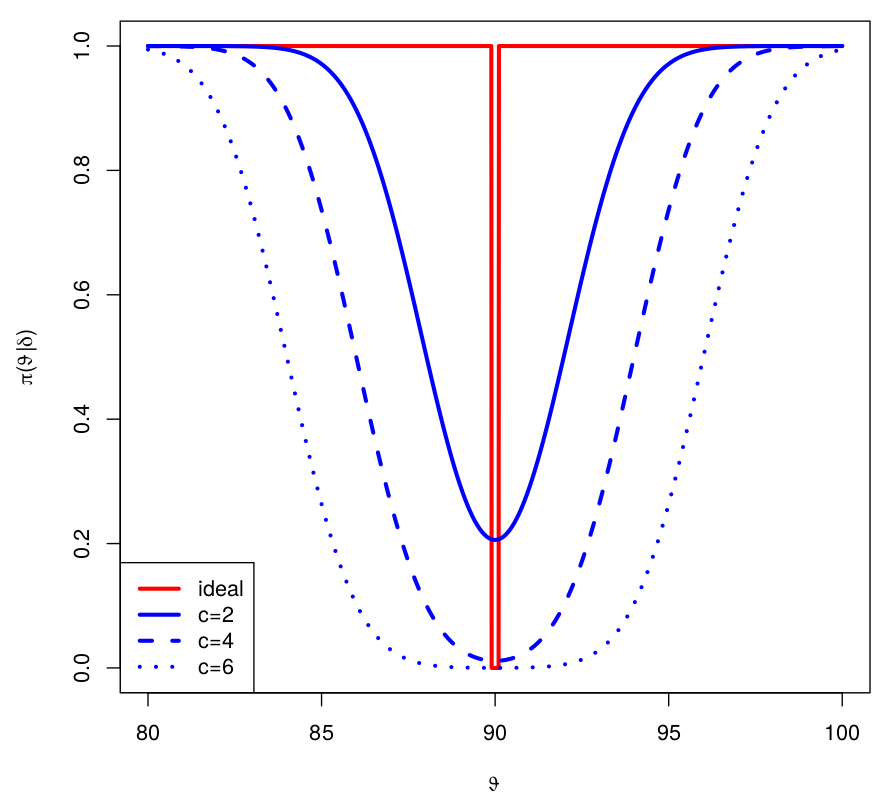
\includegraphics[width=0.5\textwidth]
                    {./figures/powerfunction.png}
                \end{figure}

                Typically, we want to design our tests in order to control the
                probability of making an error.

                \begin{definition}[Types of Error]
                    A \textbf{type I error} occurs if we decide to reject a true
                    null $H_0$. A \textbf{type II error} occurs if we fail to
                    reject a false null $H_0$.

                    Therefore, if $\theta \in \Omega_0$, then $\pi(\theta |
                    \delta)$ is the probability of a type I error (conditional
                    on $\Theta = \theta$), and if $\theta \in \Omega_1$, then $1
                    - \pi(\theta | \delta)$ is the probability of a type II
                    error (conditional on $\Theta = \theta$).

                    Since either $\theta \in \Omega_0$, or $\theta \in
                    \Omega_1$, but not both, only one type of error is possible.
                    However, we can't know which type of error we're actually
                    making, since we don't know $\theta$.

                    If we can choose between different tests, then we want
                    $\pi(\theta | \delta)$ to be low for $\theta \in \Omega_0$,
                    and high for $\theta \in \Omega_1$.

                    Normally, the hypotheses are arranged in such a way that a
                    type I error is the most important one to be avoided, so we
                    focus on that one first.
                \end{definition}

        \subsection{Level of Significance and Size of a Test}
            \begin{definition}[]
                A test $\delta$ has \textbf{level of significance} $\alpha_0$
                when $\pi(\theta | \delta) \leq \alpha_0 \, \fa \, \theta \in
                \Omega_0$ (i.e: when the probability of a type I error given
                $\Theta = \theta$ does not exceed $\alpha_0$). We also say that
                ``$\delta$ is a level $\alpha_0$ test''.

                The \textbf{size} of a test $\delta$ i:

                \[
                    \alpha(\delta) = \sup_{\theta \in \Omega_0} \pi(\theta |
                    \delta) = \min \{\alpha_0: \pi(\theta | \delta) \leq
                    \alpha_0 \, \fa \, \theta \in \Omega_0\}
                \]

                Note that, if $H_0$ is simple, (i.e: $\Omega_0 = \{\theta_0\}$),
                then $\alpha(\delta) = \pi(\theta_0 | \delta)$.

                We won't use the level of significance at all in this course,
                the size is just better, but we need to know about it because
                knowledge of it will be assumed in later years.
            \end{definition}

            \subsubsection{Example}
                \textit{Assume $X_i | \theta \sim \mathcal{U}(0, \theta)$, where
                $\theta$ is unknown, assuming $X_i$ are IID conditional on
                $\Theta$. Say we want to test $H_0: 3 \leq \Theta \leq 4$ vs
                $H_1: \Theta < 3$ or $\theta > 4$.}

                We'll define $Y_n$ as follows:

                \[
                    Y_n := \max\{X_1, ..., X_n\}
                \]

                This is the maximum likelihood estimator for $\Theta$. We say
                we'll reject $H_0$ when $Y_n < 2.5$, or when $Y_n > 4$ (4
                suffices here, since we know as soon as we see 4 we can reject
                the null hypothesis. However, three does not suffice for the
                lower bound).

                The power function for this scenario is then given by:

                \begin{align*}
                    \pi(\theta | \delta) & = \bb{P}(Y_n < 2.5 \lor Y_n > 4 |
                        \Theta = \theta) \\
                    & = \bb{P}(Y_n < 2.5 | \Theta = \theta) + 1 - \bb{P}(Y_n
                        \leq 4 | \Theta = \theta) \\
                    & = \begin{cases}
                        1 + 1 - 1 = 1, & \theta \leq 2.5 \\
                        \left(\frac{2.5}{\theta}\right)^n + 1 - 1 = \left
                            (\frac{2.5}{\theta}\right)^n, & 2.5 \leq \theta \leq
                            4 \\
                        \left(\frac{2.5}{\theta}\right)^n + 1 -
                            \left(\frac{4}{\theta}\right)^n, & \theta \geq 4
                    \end{cases}
                \end{align*}

                We can then find the size:

                \begin{align*}
                    a(\delta) & = \sup_{\theta \in \Omega_0} \pi(\theta |
                        \delta) \\
                    & = \sup_{3 \leq \theta \leq 4} \pi(\theta | \delta) \\
                    & = \pi(\theta = 3 | \delta) \quad \textit{(because
                        $\pi(\theta | \delta)$ is decreasing in $\theta \in [3,
                        4]$)}
                \end{align*}

            \subsubsection{Optimising Tests}

                If $T$ is a test statistic and our test $\delta$ is of the form
                ``reject $H_0$ when $T \geq c$'', then:

                \[
                    \alpha(\delta) = \sup_{\theta \in \Omega_0} \bb{P}(T \geq c
                    | \theta)
                \]

                This will decrease with increasing values of $c$! So, to get a
                small value of $\alpha(\delta)$ (i.e: a small size/probability
                of type I errors), we need a large value of $c$.

                However, we also want the power function $\bb{P}(T \geq c |
                \theta)$ to be large (i.e: close to 1) for $\theta \in
                \Omega_1$. Therefore, $c$ should not be too large either.

                So, picking $c$ is a tradeoff. One solution is to pick the
                smallest possible value for $c$ such that the size is equal to
                some pre-specified value $\alpha_0 \in [0, 1]$. This limits the
                worst case type II error probability, and fixes the type I error
                probability $\alpha_0$.

                \paragraph{Example}
                    Consider again our battery problem, assuming that $\sigma =
                    5$ is known, and $X_i | \theta \sim \mathcal{N}(\theta,
                    \sigma^2)$ are IID conditional on $\Theta$. Say we reject
                    $H_0: \Theta = \theta_0$, with $\theta_0 = 90$, when
                    $|\overline X_n - \theta_0| \geq c$. Then, the size of the
                    test is:

                    \begin{align*}
                        \alpha(\delta) & = \pi(\theta_0 | \delta) \\
                        & = \bb{P}(|\overline X_n - \theta_0| \geq c | \Theta =
                            \theta_0) \\
                        & = \bb{P}\left(\left.\left|\frac{\overline X_n -
                            \theta_0}{\sigma/\sqrt{n}}\right| \geq
                            \frac{c}{\sigma/\sqrt{n}}\right|\Theta = \theta_0
                            \right)
                    \end{align*}

                    This is a standard normal distribution, and this probability
                    is equal to $\alpha_0$ when:

                    \[
                        \frac{c\sqrt{n}}{\sigma} = \Phi^{-1}\left(1 -
                        \frac{\alpha_0}{2}\right) = z_{\alpha_0/2}
                    \]

                    So $c = z_{\alpha_0/2} \frac{\sigma}{\sqrt{n}} = 1.96 \cdot
                    \frac{5}{\sqrt{10}} \approx 3.1$ for $\alpha_0 = 0.05$.

        \subsection{The $p$-value}
            When testing, the outcome of the test (whether or not to reject)
            depends on our choice of significance level, $\alpha_0$. Different
            people might choose to use different values of $\alpha_0$. So,
            instead of reporting whether or not \textit{we} rejected $H_0$ at
            level $\alpha_0$, we instead report the $p$-value, defined as
            follows:

            \begin{definition}[$p$-value]
                The \textbf{p-value} is the smallest level $\alpha_0$ under
                which we would reject $H_0$ at level $\alpha_0$ with the
                observed data.

                It's probably better to think about this in terms of
                \textit{size}: so the smallest \textit{size} at which we would
                reject $H_0$ for the test with size $\alpha_0$ with the observed
                data.
            \end{definition}

            \subsubsection{Example}
                In the battery example, we observed $\overline x_n = 86.8$. Note
                that $|86.8 - 90| > 3.1$, so we would reject $H_0: \Theta = 90$
                at the 0.05 level. Instead however, we could report the
                $p$-value: For any given level $\alpha_0$, we know we will
                reject $H_0$ if:

                \[
                    |\overline x_n - \theta_0| \geq z_{\alpha/2}
                    \frac{\sigma}{\sqrt{n}}
                \]

                Or equivalently, when:

                \[
                    2.02 = \left|\frac{\overline x_n - \theta_0}
                    {\sigma/\sqrt{n}}\right| \geq z_{\alpha_0/2} = \Phi^{-1}(1 -
                    \alpha_0/2)
                \]

                So we need $\Phi(2.02) \geq 1 - \frac{\alpha_0}{2}$.

                The smallest value of $\alpha_0$ for which this is satisfied is
                $\alpha_0 = 2(1 - \Phi(2.02)) = 0.043$. So the $p$-value is
                $0.043$, and therefore we would reject at all levels $\alpha_0
                \geq 0.043$.

            \subsubsection{Theorem}
                For tests of the form ``reject $H_0$ when $T \geq c$'', the
                $p$-value is equal to:

                \[
                    \sup_{\theta \in \Omega_0} \bb{P}(T \geq t | \theta)
                \]

                where $t$ is the actual observed value of the test statistic
                $T$.

                \paragraph{Proof}
                    We will reject the null hypothesis at the level $\alpha_0$
                    when $t \geq c$ for $c$ satisfying:

                    \[
                        \pi(\theta | \delta) = \bb{P}(T \geq c | \theta) \leq
                        \alpha_0 \, \fa \, \theta \in \Omega_0
                    \]

                    So, the $p$-value is:

                    \begin{align*}
                        \min\{\alpha_0: \bb{P}(T \geq c | \theta) \leq \alpha_0
                            \, \fa \, \theta \in \Omega_0, t \geq c\} & =
                            \min\{\sup_{\theta \in \Omega_0} \bb{P}(T \geq c |
                            \theta): t \geq c\} \\
                        & = \sup_{\theta \in \Omega_0} \bb{P}(T \geq t | \theta)
                    \end{align*}

                    This final equality holds as  $\sup\limits_{\theta \in
                    \Omega_0} \bb{P}(T \geq c | \theta)$ is a decreasing
                    function of $c$, so we should take $c$ to be as large as
                    possible to minimise this. From the inequality $t \geq c$,
                    the largest possible value of $c$ will be $t$.

                \paragraph{Example}
                    In the battery example, we can check that the $p$-value is:

                    \begin{align*}
                        \sup_{\theta \in \Omega_0} \bb{P}(|\overline X_n -
                            \theta_0| \geq |86.8 - \theta_0| | \theta_0) & =
                            \bb{P}(|\overline X_n - 90| \geq 3.2 | \Theta = 90)
                            \\
                        & = \bb{P}\left(\left.\left|\frac{\overline X_n - 90}
                            {5/\sqrt{10}}\right| \geq \frac{3.2}{5/\sqrt{10}}
                            \right | \Theta = 90 \right) \\
                        & = \bb{P}\left(\left.\left|\frac{\overline X_n - 90}
                            {5/\sqrt{10}}\right| \geq 2.02 \right | \Theta = 90
                            \right) \\
                        & = 2(1 - \Phi(2.02)) \\
                        & = 0.043
                    \end{align*}

                    We already found 0.043 to be the $p$-value, so we can see
                    that the theorem works here.

    \newpage
    \section{Bayesian Analysis of Normal Sampling with Unknown Mean, Unknown
    Variance}
        \begin{fread}
            [DS12, section 8.6]
        \end{fread}

        \subsection{Likelihood}
            We assume that we have $X_i | \mu, \tau \sim \mathcal{N}\left(\mu,
            \frac{1}{\tau}\right)$ IID conditional on $M, T$, corresponding to
            the parameters. Recall that $\tau$ is the precision parameter, with
            $\frac{1}{\tau} = \sigma^2$. $M$ is the random variable
            corresponding to $\mu$, and $T$ is the random variable corresponding
            to $\tau$. We observe a sample $x_1, ..., x_n$ to learn about $M$
            and $T$.

            First, recall Bayes's theorem:

            \begin{align*}
                \text{posterior dist } & \propto \text{ prior dist } \cdot
                    \text{ likelihood } \\
                f(\mu, \tau | x_1, ..., x_n) & \propind{\mu, \tau} f(\mu, \tau)
                    \cdot f(x_1, ..., x_n | \mu, \tau)
            \end{align*}

            We know that the likelihood is given by the product:

            \[
                f(x_1, ..., x_n | \mu, \tau) = \prod_{i=1}^n f(x_i | \mu, \tau)
            \]

            We further know that:

            \[
                f(x_i | \mu, \tau) = \sqrt{\frac{\tau}{2\pi}}
                \exp\left(-\frac{1}{2}\tau (x_i - \mu)^2\right)
            \]

            So we have the formula for the likelihood:

            \[
                f(x_1, ..., x_n | \mu, \tau) = \left(\frac{\tau}{2\pi}\right)
                ^{n/2} \exp\left(-\frac{1}{2}\tau \sum_{i=1}^n (x_i - \mu)^2
                \right)
            \]

        \subsection{The Normal-Gamma Prior}
            Suppose we assign the following prior distributions to $M$ and $T$:

            \[
                M | \tau \sim \mathcal{N}\left(\mu_0, \frac{1}{\lambda_0 \tau}
                \right), \quad T \sim \mathrm{Gamma}(\alpha_0, \beta_0)
            \]
            \begin{align*}
                \implies f(\mu | \tau) & = \sqrt\frac{\lambda_0\tau}{2\pi}
                    \exp\left(-\frac{1}{2}\lambda_0\tau(\mu - \mu_0)^2\right) \\
                f(\tau) & = \frac{\beta_0^{\alpha_0}} \tau^{\alpha_0 - 1}
                    \exp(-\beta_0 \tau) \\
                f(\mu, \tau) & = f(\mu | \tau) f(\tau) \\
                & \propind{\mu, \tau} \tau^{\alpha_0 - 1/2} \exp\left(-\tau
                    \left(\beta_0 + \frac{\lambda_0}{2}(\mu - \mu_0)^2\right)
                    \right)
            \end{align*}

            This is called the \textbf{normal-gamma prior} for $M$ and $T$, with
            hyper-parameters $\mu_0 \in \R, \lambda_0 > 0, \alpha_0 > 0, \beta_0
            > 0$.

            We notate this as:

            \[
                (M, T) \sim \text{Normal Gamma}(\mu_0, \lambda_0, \alpha_0,
                \beta_0)
            \]

            We have that:

            \[
                \E(M | \tau) = \mu_0
            \]
            \[
                \E(M) = \mu_0 \text{ if } \alpha_0 > \frac{1}{2}
            \]
            \[
                \E(T) = \frac{\alpha_0}{\beta_0}
            \]
            \[
                \E\left(\frac{1}{T}\right) = \frac{\beta_0}{\alpha_0 - 1}
                \text{ if } \alpha_0 > 1
            \]
            \[
                \var(M | \tau) = \frac{1}{\lambda_0 \tau}
            \]
            \[
                \var(M) = \frac{\beta_0}{\lambda_0(\alpha_0 - 1)} \text{ if }
                \alpha_0 > 0
            \]
            \[
                \var(T) = \frac{\alpha_0}{\beta_0}
            \]
            \[
                \var\left(\frac{1}{T}\right) = \frac{\beta_0^2}{(\alpha_0 - 1)^2
                (\alpha_0 - 2)} \text{ if } \alpha_0 > 2
            \]

            The conditions placed on some of these values imply certain
            properties by definition:

            \[
                \alpha_0 > 1 \iff \E(T)^2 > \var(T), \quad
                \alpha_0 > 2 \iff \E(T)^2 > 2\var(T), \quad
                \alpha_0 > \frac{1}{2} \iff \E(T)^2 > \frac{1}{2}\var(T)
            \]

        \subsection{Posterior Distribution and Conjugacy}
            Applying Bayes's theorem, we find:

            \begin{align*}
                f(\mu, \tau | x_1, ..., x_n) & \propind{\mu, \tau} f(\mu, \tau)
                    \cdot \prod_{i=1}^n f(x_i | \mu, \tau) \\
                & \propind{\mu, \tau} \tau^{\alpha_0 - 1/2} \exp\left(-\tau
                    \left(\beta_0 + \frac{\lambda_0}{2}(\mu - \mu_0)^2\right)
                    \right) \cdot \tau^{n/2} \exp\left(-\frac{1}{2} \tau
                    \sum_{i=1}^n (x_i - \mu)^2\right) \\
                & \propind{\mu, \tau} \tau^{\alpha_0 + n/2 - 1/2} \cdot
                    \exp\left(-\tau\left(\beta_0 + \frac{1}{2}\left(\lambda_0
                    (\mu - \mu_0)^2 + \sum_{i=1}^n (x_i - \mu)^2
                    \right)\right)\right)
            \end{align*}

            In section 5.6, we showed that $\sum\limits_{i=1}^n (x_i - \mu)^2 =
            s_n^2 + n(\overline x_n - \mu)^2$.

            Substituting this result then using Lemma 2.2.3(c), we have the
            following:

            \begin{align*}
                & \beta_0 + \frac{1}{2}\left(\lambda_0(\mu - \mu_0)^2
                    + \sum_{i=1}^n (x_i - \mu)^2 \right) \\
                & = \beta_0 + \frac{1}{2}\left(s_n^2 + (\lambda_0 + n)\left(\mu
                    - \frac{\lambda_0\mu_0 + n\overline x_n}{\lambda_0 + n}
                    \right)^2 + \left(\frac{1}{\lambda_0} + \frac{1}{n}
                    \right)^{-1}(\overline x_n - \mu_0)^2\right)
            \end{align*}

    \newpage
\section*{Problems Classes}
\addcontentsline{toc}{section}{\protect\numberline{}Problems Classes}
    \subsection*{07-Feb-2020}
    \addcontentsline{toc}{subsection}{\protect\numberline{}07-Feb-2020}
        \paragraph{11}
        \textit{$n = 100$ random samples of water from a fresh water lake
        were taken and the calcium concentration (given in milligrams per
        litre) measured. A 95\% confidence interval on the mean calcium
        concentration $\Theta$ is $[0.49, 0.82]$, where the standard
        deviation is assumed to be known}

        \textit{(a) Consider the following statement: There is a 95\% chance
        that $\Theta$ is between 0.49 and 0.82. Is this statement correct?
        Explain your answer}

            No, the statement is not correct, as the confidence interval is
            conditioned on $\theta$, so we are making a probability
            statement about the \textit{data}, not the parameter!

            \[
                \bb{P}(\bar X_n - 1.96 \frac{\sigma}{\sqrt{n}} \leq \theta
                \leq \bar X_n + 1.96 \frac{\sigma}{\sqrt{n}}) = 0.95
            \]

            From the information we know, the probability $\bb{P}(0.49 \leq
            \Theta \leq 0.82)$ could be anywhere between 0 and 1, and
            actually depends on the prior.

            Also, $\bb{P}(0.49 \leq \theta \leq 0.82 | \theta)$ will be
            either 0 or 1 depending on $\theta$.

        \textit{(b) The process of taking $n = 100$ random samples of water
        from the lake and computing a 95\% confidence interval on $\Theta$
        is repeated 1000 times, each time obtaining a slightly different
        interval due to randomness across the different samples. One of
        these intervals is $[0.49, 0.82]$. The true value $\theta$ of
        $\Theta$ is then revealed. Someone claims that precisely 950 of the
        1000 95\% confidence intervals computed earlier should contain
        $\theta$. Is this correct? Explain your answer.}

            This is \textit{not} correct, although we could say that it's
            ``almost'' correct. We need to remember that, ultimately, the
            number of intervals that will contain $\theta, Y,$ is a random
            variable, and is not known in advance. $Y$ may be thought of as
            a sum of Bernoulli variables:

            \[
                Y = \sum_{i=1}^{1000} I_{A_i}, \quad A_i =\{\overline
                X_{n,i} - 1.96 \frac{\sigma}{\sqrt{n}} \leq \Theta \leq ...
                + 1.96 ... \}
            \]

            If conditional on $\Theta = \theta, Y$ will still not have a
            fixed value! Recall:

            \[
                I_{A_i}(\omega) := \begin{cases}1, & \omega \in A_i \\ 0, &
                \omega \not \in A_i\end{cases}
            \]

            Note that $\bb{P}(A_i | \theta) = 0.95$.

        \textit{(c) Let $Y$ denote the number of 1000 95\% confidence
        intervals that contain $\Theta$. Identify the unconditional
        distribution of $Y$, and compute its unconditional mean and standard
        deviation. Finally, identify two numbers $a, b$ such that
        (approximately) $\bb{P}(a \leq Y \leq b) = 0.95$.}

            By (b), we have:

            \[
                Y | \theta \sim \text{Bin}(1000, 0.95)
            \]

            Because this conditional distribution doesn't depend on
            $\Theta$, by the partition theorem, we have:

            \[
                p(y) = \int_0^1 p(y | \theta) f(\theta) d\theta =
                p(y | \theta)
            \]

            Note that $p(y | \theta)$ doesn't depend on $\theta$, so we have

            \[
                p(y) = p(y | \theta) \int_0^1 f(\theta) d\theta
            \]

            So, $Y \sim \text{Bin}(1000, 0.95)$.

            Note that $\E(Y) = 1000 \cdot 0.95 = 950, \var(Y) = 1000 \cdot
            0.95 \cdot 0.05 = 6.89^2$.

            Since we have a large $n$, we may approximate the binomial
            distribution by the normal distribution, so approximately:

            \[
                Y \sim \mathcal{N}(950, 6.89^2)
            \]

            Therefore, a 95\% interval on $Y$ can be calculated:

            \[
                \bb{P}(950 - 1.96 \cdot 6.89 \leq Y \leq 950 + 1.96 \cdot
                6.89) = 0.95
            \]
            \[
                [936.5, 963.5]
            \]

        \paragraph{22}
        \textit{Consider again the conditions of exercise 21, and assume the
        same prior distribution of $\Theta$. Suppose now, however, that six
        observations are selected at random from the uniform distribution
        $[\theta - 1/2, \theta + 1/2]$, and their values are $11.0, 11.5,
        11.7, 11.1, 11.4, 10.3$. Determine the posterior distribution}.

            We have $X_i | \theta \sim \mathcal{U}(\theta - 1/2, \theta +
            1/2)$, and the prior $\Theta \sim \mathcal{U}(10, 20)$.

            \[
                f(\theta | x_1, ..., x_n) \propind{\theta} f(\theta)
                \prod_{i=1}^n f(x_i | \theta)
            \]

            where $f(\theta) \propind{\theta} \begin{cases}1, & \theta \in
            [10, 20] \\ 0, &\text{otherwise}\end{cases}$.

            \[
                \implies f(x_i | \theta) = \begin{cases}1, & x_i \in [\theta
                - 1/2, \theta + 1/2] \\ 0, & \text{otherwise}\end{cases}
            \]

            $x_i \in [\theta - 1/2, \theta + 1/2] \iff \theta \in [x_i -
            1/2, x_i + 1/2]$, so we have:

            \[
                f(\theta | x_1, ..., x_n) \propind{\theta} \begin{cases}1, &
                \theta \in [10, 20] \land \theta \in [x_i - 1/2, x_i + 1/2]
                \,\fa i = 1, ..., n \\ 0, & \text{otherwise}\end{cases}
            \]

            The first condition of this piecewise function holds $\iff
            \theta \in [10, 20] \cap \bigcap\limits_{i=1}^n [x_i - 1/2, x_i
            + 1/2] \iff \theta \in [10] \cap [\max\limits_{i=1}^n x_i - 1/2,
            \min\limits_{i=1}^n x_i + 1/2]$. Let $x^* = \max\limits_{i=1}^n
            x_i, x_* = \min\limits_{i = 1}^n x_i$ So we have:

            \[
                \Theta | x_1, ..., x_n \sim \mathcal{U}(x^* - 1/2, x_* +
                1/2) = \mathcal{U}(11.2, 11.4)
            \]

        \paragraph{33}
        \textit{Let $\theta$ denote the average number of defects per 100
        feet of a certain type of magnetic tape. Suppose that the value of
        $\theta$ is unknown and that the prior distribution of $\Theta$ is
        the gamma distribution with parameters $\alpha_0 = 2, \beta_0 = 10$.
        When a 1200-foot roll of this tape is inspected, exactly four
        defects are found. Determine the posterior distribution of
        $\Theta$.}
            \begin{relq}
                Consider exercise 31 first!
            \end{relq}

            We could pretend that instead of one 1200 foot roll, we instead
            have 12 one foot rolls, with a total of $\sum\limits_{i=1}^{12}
            x_i = 4$ defects. Therefore, by exercise 31, the posterior
            distribution is:

            \[
                \text{Gamma}\left(\alpha_0 + \sum\limits_{i=1}^{n} x_i,
                \beta_0 + n\right) = \text{Gamma}(3 + 4, 1 + 12) =
                \text{Gamma}(7, 13)
            \]

    \subsection*{21-Feb-2020}
    \addcontentsline{toc}{subsection}{\protect\numberline{}21-Feb-2020}
        \paragraph{38}
        \textit{In a clincal trial, let the probability of successful
        outcome $\Theta$ have a prior distribution that is the uniform
        distribution on the interval $[0, 1]$, which is also the beta
        distribution with parameters $1$ and $1$. Suppose that the first
        patient has a successful outcome. Find the Bayes estimate of
        $\Theta$ under squared error loss.}

            We have the prior $\Theta \sim \mathcal{U}(0, 1) =
            \text{Beta}(1, 1)$, and the sampling $X_i | \theta \sim
            \text{Bernoulli}(\theta)$. We have $n = 1, x_1 = 1$. From
            lectures, we have $\widehat \theta = \E(\Theta | x_1, ...,
            x_n)$, so the question is actually just asking us to find the
            posterior expectation under squared error loss.

            By conjugacy, we have $\Theta | x_1 \sim \text{Beta}(1 + 1, 1 +
            1 - 1) = \text{Beta}(2, 1)$, since $\alpha_1 = \alpha_0 + x_1,
            \beta_1 = \beta_0 + n - x_1$.

            By the properties of the beta distribution, we have:

            \[
                \E(\Theta | x_1) = \frac{\alpha_1}{\alpha_1 + \beta_1} =
                \frac{2}{3}
            \]

        \paragraph{41}
        \textit{A random sample of size $n$ is taken from the Bernoulli
        distribution with parameter $\theta$, which is unknown. The prior
        distribution for $\theta$ is a beta distribution for which the mean
        is $\mu_0$. Show that the mean of the posterior expectation of
        $\Theta$ will be a weighted average of the form $\gamma_n \overline
        x_n + (1 - \gamma_n)\mu_0$, and show that $\gamma_n \to 1$ as $n \to
        \infty$.}

            We have sampling $X_i | \theta \sim \text{Bernoulli}(\theta)$,
            with prior $\Theta \sim \text{Beta}(\alpha_0, \beta_0)$.
            Therefore, $\E(\Theta) = \frac{\alpha_0}{\alpha_0 + \beta_0} =
            \mu_0$.

            By conjugacy, we have:

            \begin{align*}
                \E(\Theta | x_1, ..., x_n) & = \frac{\alpha_n}{\alpha_n +
                    \beta_n} \\
                & = \frac{\alpha_0 + \sum\limits_{i=1}^n x_i} {\alpha_0 +
                    \beta_0 + n} \\
                & = \frac{\alpha_0}{\alpha_0 + \beta_0 + n} + \frac{n}
                    {\alpha_0 + \beta_0 + n}\overline x_n
            \end{align*}

            Is the denominator $\alpha_0 + \beta_0 + n$ equal to $\gamma_n$?
            Yes, if the first fraction $\frac{\alpha_0}{\alpha_0 + \beta_0 +
            n}$ is equal to $(1 - \gamma_n)\mu_0$.

            We can check this:

            \begin{align*}
                (1 - \gamma_n)\mu_0 & = \frac{\alpha_0 + \beta_0}{\alpha_0 +
                    \beta_0 + n} \cdot \frac{\alpha_0}{\alpha_0 + \beta_0}\\
                & = \frac{\alpha_0}{\alpha_0 + \beta_0 + n}
            \end{align*}

            So yes, we've demonstrated that this is a weighted average.

        \paragraph{49}
        \textit{It is not known what proportion $\Theta$ of the purchases of
        a certain brand of breakfast cereal are made by women, and what
        proportion are made by men. In a random sample of 70 purchases of
        this cereal, it was found that 58 were made by women and 12 were
        made by men.}

        \textit{(a) Find the maximum likelihood estimator of $\Theta$.}

            We are doing Bernoulli sampling. Let $X_i$ equal $1$ if female,
            $0$ if male. Then $X_i | \theta \sim \text{Bernoulli}(\theta)$.

            For this sampling, the MLE is therefore $\widehat \theta =
            \frac{\sum\limits_{i=1}^n x_i}{n} \approx 0.83$.

        \textit{(b) Now suppose that it is additionally known that
        $\frac{1}{2} \leq \Theta \leq \frac{2}{3}$. What is now the maximum
        likelihood likelihood estimator of $\Theta$? (Hint: When is
        $L'(\theta) > 0$?)}

            Let's answer the hint first, since if we want to maximise this
            function, we just need to maximise the log likelihood.

            \[
                L(\theta) = y\log\theta + (n - y)\log(1 - \theta), \quad y =
                \sum_{i=1}^n x_i
            \]
            \begin{align*}
                & L'(\theta) > 0 \\
                \iff & \frac{y}{\theta} - \frac{n - y}{1 - \theta} > 0 \\
                \iff & (1 - \theta)y - \theta(n - y) > 0 \\
                \iff & y - n\theta > 0 \\
                \iff & \theta < \frac{y}{n} = \frac{58}{70} \approx 0.83
            \end{align*}

            So the maximum of the log likelihood $L(\theta)$ over
            $\left[\frac{1}{2}, \frac{2}{3}\right]$ is achieved at $\widehat
            \theta = \frac{2}{3}$ (as the gradient is always positive, so
            the function is strictly increasing).

        \paragraph{50}
        \textit{Suppose that $X_1, ..., X_n$ form a random sample from a
        Poisson distribution for which the mean $\theta$ is unknown, with
        $\theta > 0$.}

        \textit{(a) Determine the maximum likelihood estimate of $\Theta$,
        assuming that at least one of the oserved values is different from
        $0$.}

            We have sampling given by $X_i | \theta \sim \text{Po}(\theta)$,
            so $p(x_i | \theta) = \theta^{x_i} \frac{e^{-\theta}}{x_i!}$,
            and $\log{p}(x_i | \theta) = x_i\log{\theta}- \theta -
            \log(x_i!)$. So:

            \begin{align*}
                L(\theta) & = \log p(x_1, ..., x_n | \theta) \\
                & = \log\prod_{i=1}^n p(x_i | \theta) \\
                & = \sum_{i=1}^n \log p(x_i | \theta) \\
                & = \sum_{i=1}^n (x_i\log\theta - \theta - \log(x_i!)) \\
                & = \log\theta \sum_{i=1}^n x_i - n\theta - D
            \end{align*}

            where $D$ is a constant that doesn't depend on $\theta$.

            Therefore:

            \[
                L'(\theta) = \frac{\sum\limits_{i=1}^n x_i}{\theta} - n =
                \frac{n\overline x_n}{\theta} - n
            \]
            \[
                L''(\theta) = -\frac{n\overline x_n}{\theta^2}
            \]

            So $L'(\widehat \theta) = 0$ when $\widehat \theta = \overline
            x_n$, provided $x_n > 0$ (so when at least one $x_i > 0$).
            Further $L''(\overline \theta) < 0$, so it is a maximum.

        \textit{(b) Show that the maximum likelihood estimate of $\Theta$
        does not exist if every observed value is $0$.}

            If all $x_i = 0$, then $\overline x_n = 0$, and $L'(\theta) = -n
            < 0$. This achieves a maximum near $\theta = 0$, but for $\theta
            = 0, \text{Po}(\theta)$ is not a valid distribution, as
            $\widehat \theta$ does not exist in this case!

    \subsection*{06-Mar-2020}
    \addcontentsline{toc}{subsection}{\protect\numberline{}06-Mar-2020}
        \paragraph{65}
        \textit{Suppose that $X_1, ..., X_n$ form a random sample from the
        normal distribution with known mean $\mu$ and known variance
        $\sigma^2$. Let $S_n^2 := \sum\limits_{i=1}^n (X_i - \overline
        X_n)^2$. Determine the smallest value of $n$ for which the following
        relation is satisfied:}

        \[
            \bb{P}\left(\frac{S_n^2}{n\sigma^2} \leq 1.5\right) \geq 0.95
        \]

            We know from lectures that:

            \[
                Y_{n-1} := \frac{S_n^2}{\sigma^2} \sim \chi^2(n - 1)
            \]

            Therefore, we need to find an $n$ such that:

            \[
                \bb{P}\left(\frac{S_n^2}{\sigma^2} \leq 1.5n\right) =
                \bb{P}(Y_{n-1} \leq 1.5n) \geq 0.95
            \]

            Looking at the table for the Chi-Square distribution, with $n =
            20$, we see that $\bb{P}(Y_{n-1} \leq 30.14) = 0.95$, so we must
            have $\bb{P}(Y_{n-1} \leq 1.5n = 30) < 0.95$. Therefore, $n =
            21$ is the lowest value of $n$ satisfying the inequality.

        \paragraph{68}
        \textit{Suppose that the five random variables $X_1, ..., X_5$ are
        IID and that each has the standard normal distribution. Determine a
        constant $c$ such that the random variable given by:}

        \[
            \frac{c(X_1 + X_2)}{(X_3^2 + X_4^2 + X_5^2)^{1/2}}
        \]

        \textit{will have a $t$ distribution.}

            If $X \sim \mathcal{N}(0, 1)$, and $Y \sim \chi^2(n)$ are
            independent, then $\frac{X}{\sqrt{Y}{n}} \sim t(n)$. Now note the
            following:

            \[
                \frac{1}{\sqrt{2}} (X_1 + X_2) \sim \mathcal{N}(0, 1)
            \]
            \[
                (X_3^2 + X_4^2 + X_5^2) \sim \chi^2(3)
            \]

            Therefore, we have:

            \[
                \frac{1/\sqrt{2} \cdot (X_1 + X_2)}{\sqrt{1/3 \cdot (X_3^2 +
                X_4^2 + X_5^2)}} \sim t(3) \implies c = \sqrt{\frac{3}{2}}
            \]

        \paragraph{73}
        \textit{Show that, for normal sampling with unknown mean $\mu$ and
        unknown variance $\sigma^2$, for large $n$, we approximately have
        that:}

        \[
            \bb{P}\left(\left.n - 1 - z_{\alpha/2}\sqrt{2(n - 1)} \leq
            \frac{S_n^2}{\sigma^2} \leq n - 1 + z_{\alpha/2}\sqrt{2(n - 1)}
            \right|\mu, \sigma^2\right) = 1 - \alpha
        \]

        \textit{where $z_{\alpha/2} := \Phi^{-1}(1 - \alpha/2)$ as usual.}

            For large $n$, by the CLT, we have:

            \[
                \left.\frac{S_n^2}{\sigma^2}\right|\mu, \sigma^2 \sim
                \chi^2(n -1) \approx \mathcal{N}(n - 1, 2(n - 1))
            \]

            since $\E(y) = n, \var(Y) = 2n$ for $Y \sim \chi^2(n)$.

            \begin{align*}
                & \bb{P}\left(\left.n - 1 - z_{\alpha/2}\sqrt{2(n - 1)} \leq
                    \frac{S_n^2}{\sigma^2} \leq n - 1 + z_{\alpha/2}
                    \sqrt{2(n - 1)} \right|\mu, \sigma^2\right) = 1 - \alpha
                    \\
                \iff & \bb{P}\left(\left.-z_{\alpha/2} \leq \frac{1}{\sqrt{2
                    (n-1)}}\left(\frac{S_n^2}{\sigma^2} - (n - 1)\right)
                    \leq z_{\alpha/2}\right|\mu, \sigma^2\right) = 1 -
                    \alpha
            \end{align*}

            Now note that we have the following approximate result:

            \[
                \frac{1}{\sqrt{2 (n-1)}}\left(\frac{S_n^2}{\sigma^2} - (n -
                1)\right) \sim \mathcal{N}(0, 1)
            \]

            The second statement clearly then holds, since this is a
            well-known result for the normal distribution. Therefore, the
            proposition holds.

        \paragraph{74}
        \textit{(a) Show that, for any sequence of numbers $x_1, ..., x_n$
        we have that:}

        \[
            \sum_{i=1}^n (x_i - \overline x_n)^2 = \sum_{i=1}^n x_i^2 -
            n\overline x_n^2
        \]

        \textit{where $\overline x_n := \frac{1}{n} \sum\limits_{i=1}^n x_i$
        as usual.}

            \begin{align*}
                \sum_{i=1}^n (x_i - \overline x_n)^2 & = \sum_{i=1}^n x_i^2
                    - 2\overline x_n \sum_{i=1} x_i + n \overline x_n^2 \\
                & = \sum_{i=1}^n x_i^2 - 2 n\overline x_n^2 + n \overline
                    x_n^2 \\
                & = \sum_{i=1}^n x_i^2 - n\overline x_n^2
            \end{align*}

        \textit{(b) An article in cancer research tested the tumorigenesis
        of a drug. Rats were randomly selected from litter and given the
        drug. The times of tumour appearance were recorded as follows:}

        \begin{center}
            \textit{(snipped for space, see the actual problem sheet)}
        \end{center}

        \textit{It can be verified that the number of observations is 41,
        the sum of the data is 3640, and the sum of squares of the data is
        333392. Calculate $s_n^2$ for the above data.}

            Using the above fact, we have:

            \begin{align*}
                s_n^2 & = \sum_{i=1}^n (x_i - \overline x_n)^2 \\
                & = \sum_{i=1}^n x_i^2 - n\overline x_n^2 \\
                & = 333392 - 41 \left(\frac{3640}{31}\right)^2 \\
                & = 10231.02
            \end{align*}

        \textit{(c) For the same cancer data, use the normal approximation
        to the $\chi^2$ distribution to find the observed value of a 95\%
        confidence interval for the standard deviation of time until a
        tumour appearance. Explicitly state any assumptions that you make,
        and explain why a normal approximation is justified for this case.}

            Since $n$ is large, we know the following:

            \[
                \bb{P}\left(\left.n - 1 - z_{\alpha/2} \sqrt{2(n-1)} \leq
                \frac{S_n^2}{\sigma^2} \leq n - 1 +
                z_{\alpha/2}\sqrt{2(n-1)} \right|\mu, \sigma^2\right) = 1 -
                \alpha
            \]
            \[
                \implies \bb{P}\left(\left.\sqrt{\frac{S_n^2}{n - 1 +
                z_{\alpha/2}\sqrt{2(n-1)}}} \leq \sigma \leq
                \sqrt{\frac{S_n^2}{n - 1 - z_{\alpha/2}\sqrt{2(n-1)}}}
                \right|\mu, \sigma^2\right)
            \]

            Therefore, we have an approximate confidence interval on
            $\sigma$. For our data, with $1 - \alpha = 0.95$, we find:

            \[
                \left[\sqrt{\frac{S_n^2}{n - 1 +
                z_{\alpha/2}\sqrt{2(n-1)}}},
                \sqrt{\frac{S_n^2}{n - 1 - z_{\alpha/2}\sqrt{2(n-1)}}}\,\,
                \right] = [13.34, 21.34]
            \]


\end{document}
